As mentioned in Chapter \ref{ch:introduction}, the experimental discovery of a particle consistent with the SM Higgs boson by the CMS and ATLAS experiments at the CERN LHC in 2012 marked a milestone moment in the history of particle physics. After having verified the existence of this particle, physicists
have sought to further their understanding of the Higgs boson and the underlying electroweak symmetry breaking process. Additionally, the Higgs boson
is widely explored as a potential bridge to physics beyond the standard model (BSM).

Through the investigation of Higgs pair production, the production of two Higgs bosons in a single process introduced in Section \ref{sec:Higgs_Pair_Production}, physicists can both test SM predictions and 
search for BSM. On the SM front, investigating Higgs pair production allows for a fundamental test as the shape of the Higgs potential in the SM Lagrangian 
depends on the Higgs self-coupling value described in Section \ref{sec:Higgs}, which can be directly accessed via Higgs pair production. A precise measurement of this coupling would provide the first experimental insight 
into the shape of the Higgs potential, which can have profound implications on the understanding of our world, for example by providing evidence that the Higgs vaccum expectation value sits at a 
meta-stable minimum consistent with the SM prediction. Alternatively, a measurement which is not consistent with this SM prediction could hint to physics beyond the standard model \cite{10.3389/fspas.2018.00040}. 

The main LO processes which contribute the most to the di-Higgs production cross section destructively interfere, leading to a low production cross section of about 31.05 fb at a center of mass of $\sqrt{s} = $ 13 TeV, previously explained in Section \ref{sec:Higgs_Pair_Production}. 

% The main leading order (LO) processes which contribute to the cross section of Higgs pair production in the gluon fusion production mode ($gg \to HH$) are the ``triangle'' and ``box'' diagrams, shown in Fig. \ref{SMLO_ggHH_production}. 
% The box diagram is sensitive to the top Yukawa coupling, while the triangle diagram is sensitive to both the top Yukawa and trilinear self-coupling. 
% Hence, the resulting cross-section is particularly sensitive to these parameters, whose values are precisely predicted in the SM. Assuming a self-coupling strength as predicted
% by the SM, these diagrams destructively 
% interfere, leading to a small production cross section. 

In order to search for this relatively small signal, a search is performed in the WW$\gamma\gamma$ channel. 
This final state benefits from the sensitive $H\rightarrow\gamma\gamma$ process which provides a narrow, distinguishable signature. Additionally, the
$H\rightarrow WW$ leg of the decay contributes a relatively large branching ratio among Higgs boson decays of about 22\%. 
Because the W boson can decay both leptonically (W$\rightarrow\ell\nu$) and hadronically (W$\rightarrow$qq), the $H\rightarrow WW$ and by extension the $HH\rightarrow WW\gamma\gamma$ process has three possible final states:
The fully-hadronic (FH), semi-leptonic (SL), and fully-leptonic (FL) final states, corresponding to 0, 1, and 2 leptonically decaying W-bosons respectively, whose Feynman diagrams are shown in Figure \ref{fig:HHWWgg_FD_finalStates}. 

\begin{figure}[H]%
    \setcounter{subfigure}{0} % reset subcaption counter to 0 (a) 
    \centering
    \subfloat[{\footnotesize Semi-Leptonic}]{
\includegraphics[width=.25\textwidth]{Sections/HHWWgg/images/Introduction/FD_HH_qqlnu.png}}%
    \qquad
    \subfloat[{\footnotesize Fully-Hadronic}]{
\includegraphics[width=.25\textwidth]{Sections/HHWWgg/images/Introduction/FD_HH_qqqq.png}}%
    \qquad
    \subfloat[{\footnotesize Fully-Leptonic}]{
\includegraphics[width=.25\textwidth]{Sections/HHWWgg/images/Introduction/FD_HH_lnulnu.png}}%
    \qquad
    \caption{The three decay modes of H$\rightarrow$ WW. \label{fig:HHWWgg_FD_finalStates}}%
\end{figure} 

These three final states can be identified in data and simulation
with separate selections and categorizations, and their corresponding
signal and background models can be simultaneously fit to data in order to improve the overall analysis sensitivity towards di-Higgs production. Due to the expected overlap between the FH WW$\gamma\gamma$, FH ZZ$\gamma\gamma$, and bb$\gamma\gamma$ di-Higgs
final states, an attempt is made to remove as much FH ZZ$\gamma\gamma$ and bb$\gamma\gamma$ as possible. Any residual yields from these non-WW$\gamma\gamma$ final states are considered as signal in the analysis when building simulation templates. 

In addition to the prediction of SM di-Higgs, several BSM models predict the existence of real and virtual heavy particles that can couple to a pair of Higgs bosons \cite{deFlorian:2016spz, Nakamura:2017irk, Englert:2019eyl, Robens:2019kga, Tang:2012pv}.
These can lead to the appearance of a resonant contribution to the invariant mass of the $HH$ system, or to a significant modification of Higgs boson pair production through virtual processes. As no direct searches for BSM particles have resulted in discoveries at the LHC, we choose to parameterize 
these possible effects at LHC energy scales using an Effective field theory (EFT) approach ~\cite{deFlorian:2016spz, Carvalho:2015ttv}. The effects are parametrized either as modifications to the SM couplings, 
or as contact interactions. In the SM coupling modifications, possible new resonances contribute through loop diagrams whereas the contact interaction is a way of 
describing a process where the mediator has a mass far above the momentum transfer in the event and therefore can be both via a triangular virtual loop or resonant production. 
The interpretations of this analysis include the purely SM interpretation, an EFT interpretation leading to scans of modified SM and purely BSM lagrangian coupling constants, 
and a search for 20 EFT benchmarks corresponding to points which are collectively largely representative of the explored 5-dimensional EFT phase space \cite{Carvalho:2015ttv,Buchalla:2018yce,Capozi:2019xsi}.  

This is the first search for Higgs pair production in the WW$\gamma\gamma$ final state performed by the CMS experiment, and is performed using pp collisions at $\sqrt{s} = $ 13 TeV.
The data sample corresponds to an integrated luminosity of 138 \unit{fb}$^{-1}$ collected with the CMS detector at the CERN LHC during Run 2 (2016-18).
A search in the SL WW$\gamma\gamma$ final state was performed 
by the ATLAS experiment using data collected at the LHC in 2016, where a cut-based analysis was performed to obtain an observed (expected) upper limit on SM di-Higgs
production of 7.7 (5.4) pb at a 95\% confidence level \cite{Aaboud2018}. 

The structure of this chapter is as follows: The overall strategy of the analysis is described in Section \ref{sec:Strategy}. A description of the EFT parameterization and
benchmarks is provided in Section \ref{sec:EFT_Description}. The data samples and simulated events are described in Section \ref{sec:samples}. 
The reconstruction of particles as detector objects is described in Section \ref{sec:Objects}. Event selection criteria and categorization are described in Section \ref{fig:HHWWgg_SelectionsAndCat}. 
The method of signal and background modelling using simulation and data is
described in Section \ref{sec:AnalyticFitting}. A description of the systematic uncertainties of the analysis is presented in Section \ref{section:Systematics}.
The results of the analysis are described in Section \ref{sec:results}, and a summary is provided in Section \ref{section:Summary}. 

%%%

\section{Strategy} \label{sec:Strategy}

In most searches for physical processes in particle physics data, a simulation template is formed and is then fit to data in a given signal region in order to determine if the expected physical process in present in the data. Typically the signal region is a single variable, or set of variables where more signal than background is expected. In this analysis, the signal region used to fit the simulation template to data is the diphoton invariant mass, in the window 115 $<$ $\mgg$ $<$ 135. This region is chosen due to the expectation that the H$\rightarrow\gamma\gamma$ leg of the HH$\rightarrow$WW$\gamma\gamma$ process should provide a peak in this region.

There are two background signatures present in this analysis: A resonant background from the single Higgs to $\gamma\gamma$ process, and a continuum background formed by a combination of background processes which do not contain a prompt diphoton. An illustration of the signal and background signatures is shown in Figure \ref{fig:Signatures}.

\begin{figure}[h!]
    \centering
    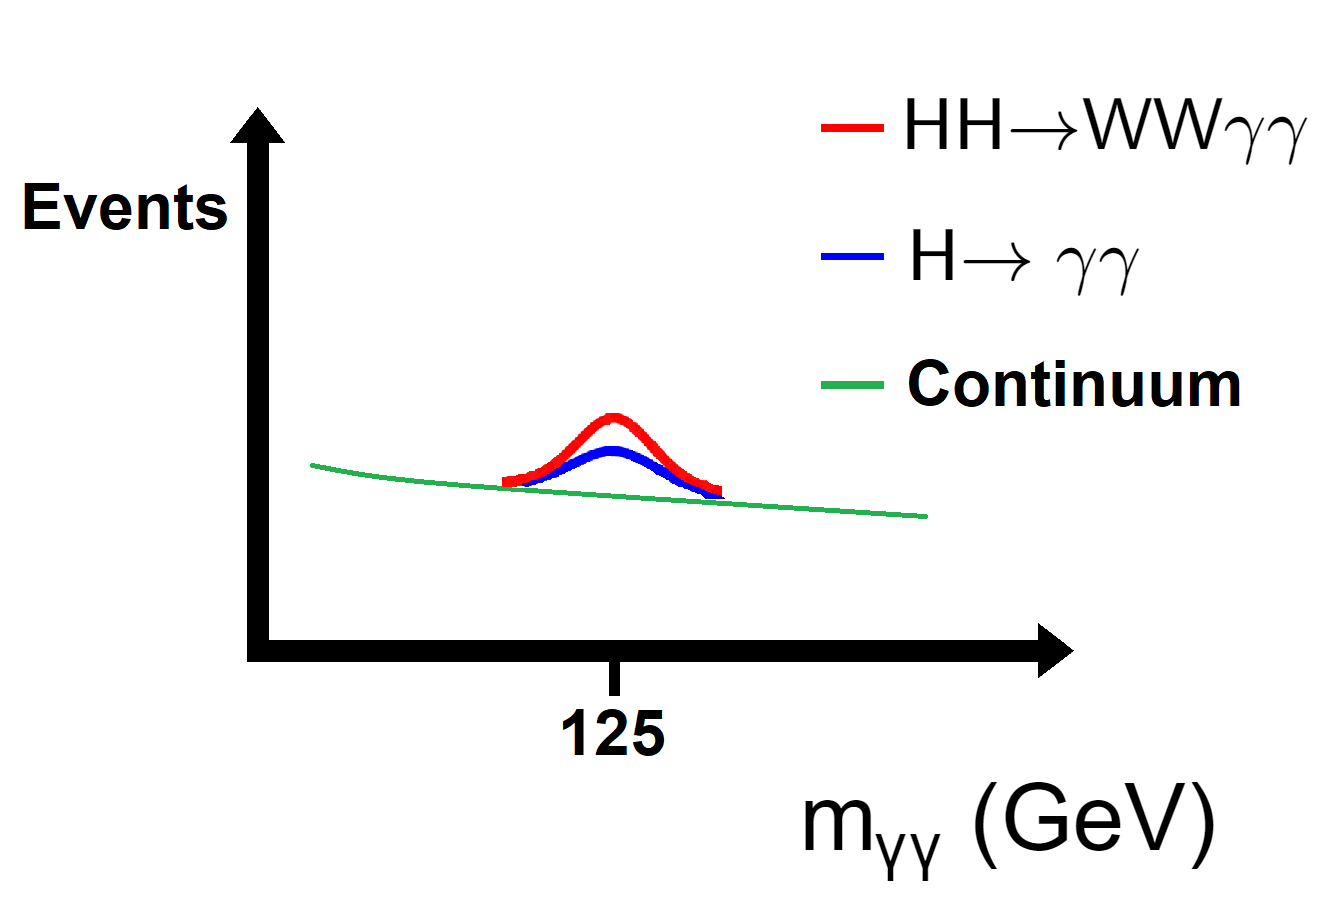
\includegraphics[width=0.75\textwidth]{Sections/HHWWgg/images/Strategy/HHWWgg_ResbkgPlot.png}
    \caption{Analysis signal and background signatures.}
    \label{fig:Signatures}
\end{figure}

In order to optimize the sensitivity of this analysis,
a DNN (Deep Neural Network) is employed for the Semi-Leptonic final state, as it is expected to be the most sensitive channel due to the increase in branching ratio
from the hadronic W decay, but with the benefit of maintaining a clean signature due to the presence of a lepton. A multiclass DNN is trained in order to separate the SM di-Higgs signal from background processes, while a binary parametric DNN is used to differentiate 20 EFT benchmark scenarios from background processes.

The FH channel also uses a DNN in order to optimize sensitivity, in this case by separating FH HH signal from backgrounds. In the FH channel, there is a significant overlap with the $HH\rightarrow$bb$\gamma\gamma$ final state, so two binary DNNs are trained:
The first binary DNN separates the FH WW$\gamma\gamma$ process from all backgrounds, and is used for categorization. To reduce the overlap of bb$\gamma\gamma$ events between the bb$\gamma\gamma$ and WW$\gamma\gamma$ phase spaces,
another binary DNN is trained that separates bb$\gamma\gamma$ from all backgrounds. The bb$\gamma\gamma$ training score is used as a ``bb$\gamma\gamma$ killer'', where a selection is applied on its value
to reduce the contamination of bb$\gamma\gamma$ events in the WW$\gamma\gamma$ phase space, while preserving the majority of WW$\gamma\gamma$ signal events. 

For the Fully-Leptonic channel, a cut based strategy is used due to a lack of number of events necessary to perform an MVA (Multivariate analysis) training. 

It is imperative to apply orthogonal selections to data and simulation events in order to avoid including the same events in multiple background categories. This is done via the event's number of leptons, where
each lepton must pass a common set of selections applied for all final state tags. After a set of lepton objects is selected for each data or simulation event, events fall into the FH category if they contain exactly zero leptons, the SL category if they contain exactly one lepton and the FL category if they contain exactly two leptons.

Further event selections are made for the three final state categories,
but by requiring an orthogonal separation of the number of leptons, it is guaranteed no one event can fall into more than one category. Thus, a simultaneous fit of background and signal models to data 
in different final state categories can be performed in order to obtain a final result which benefits from a combination of the physics signatures of all three final states. This is also summarised in the flow chart shown in Figure \ref{fig:HHflowChart}.

\begin{figure}[h!]
    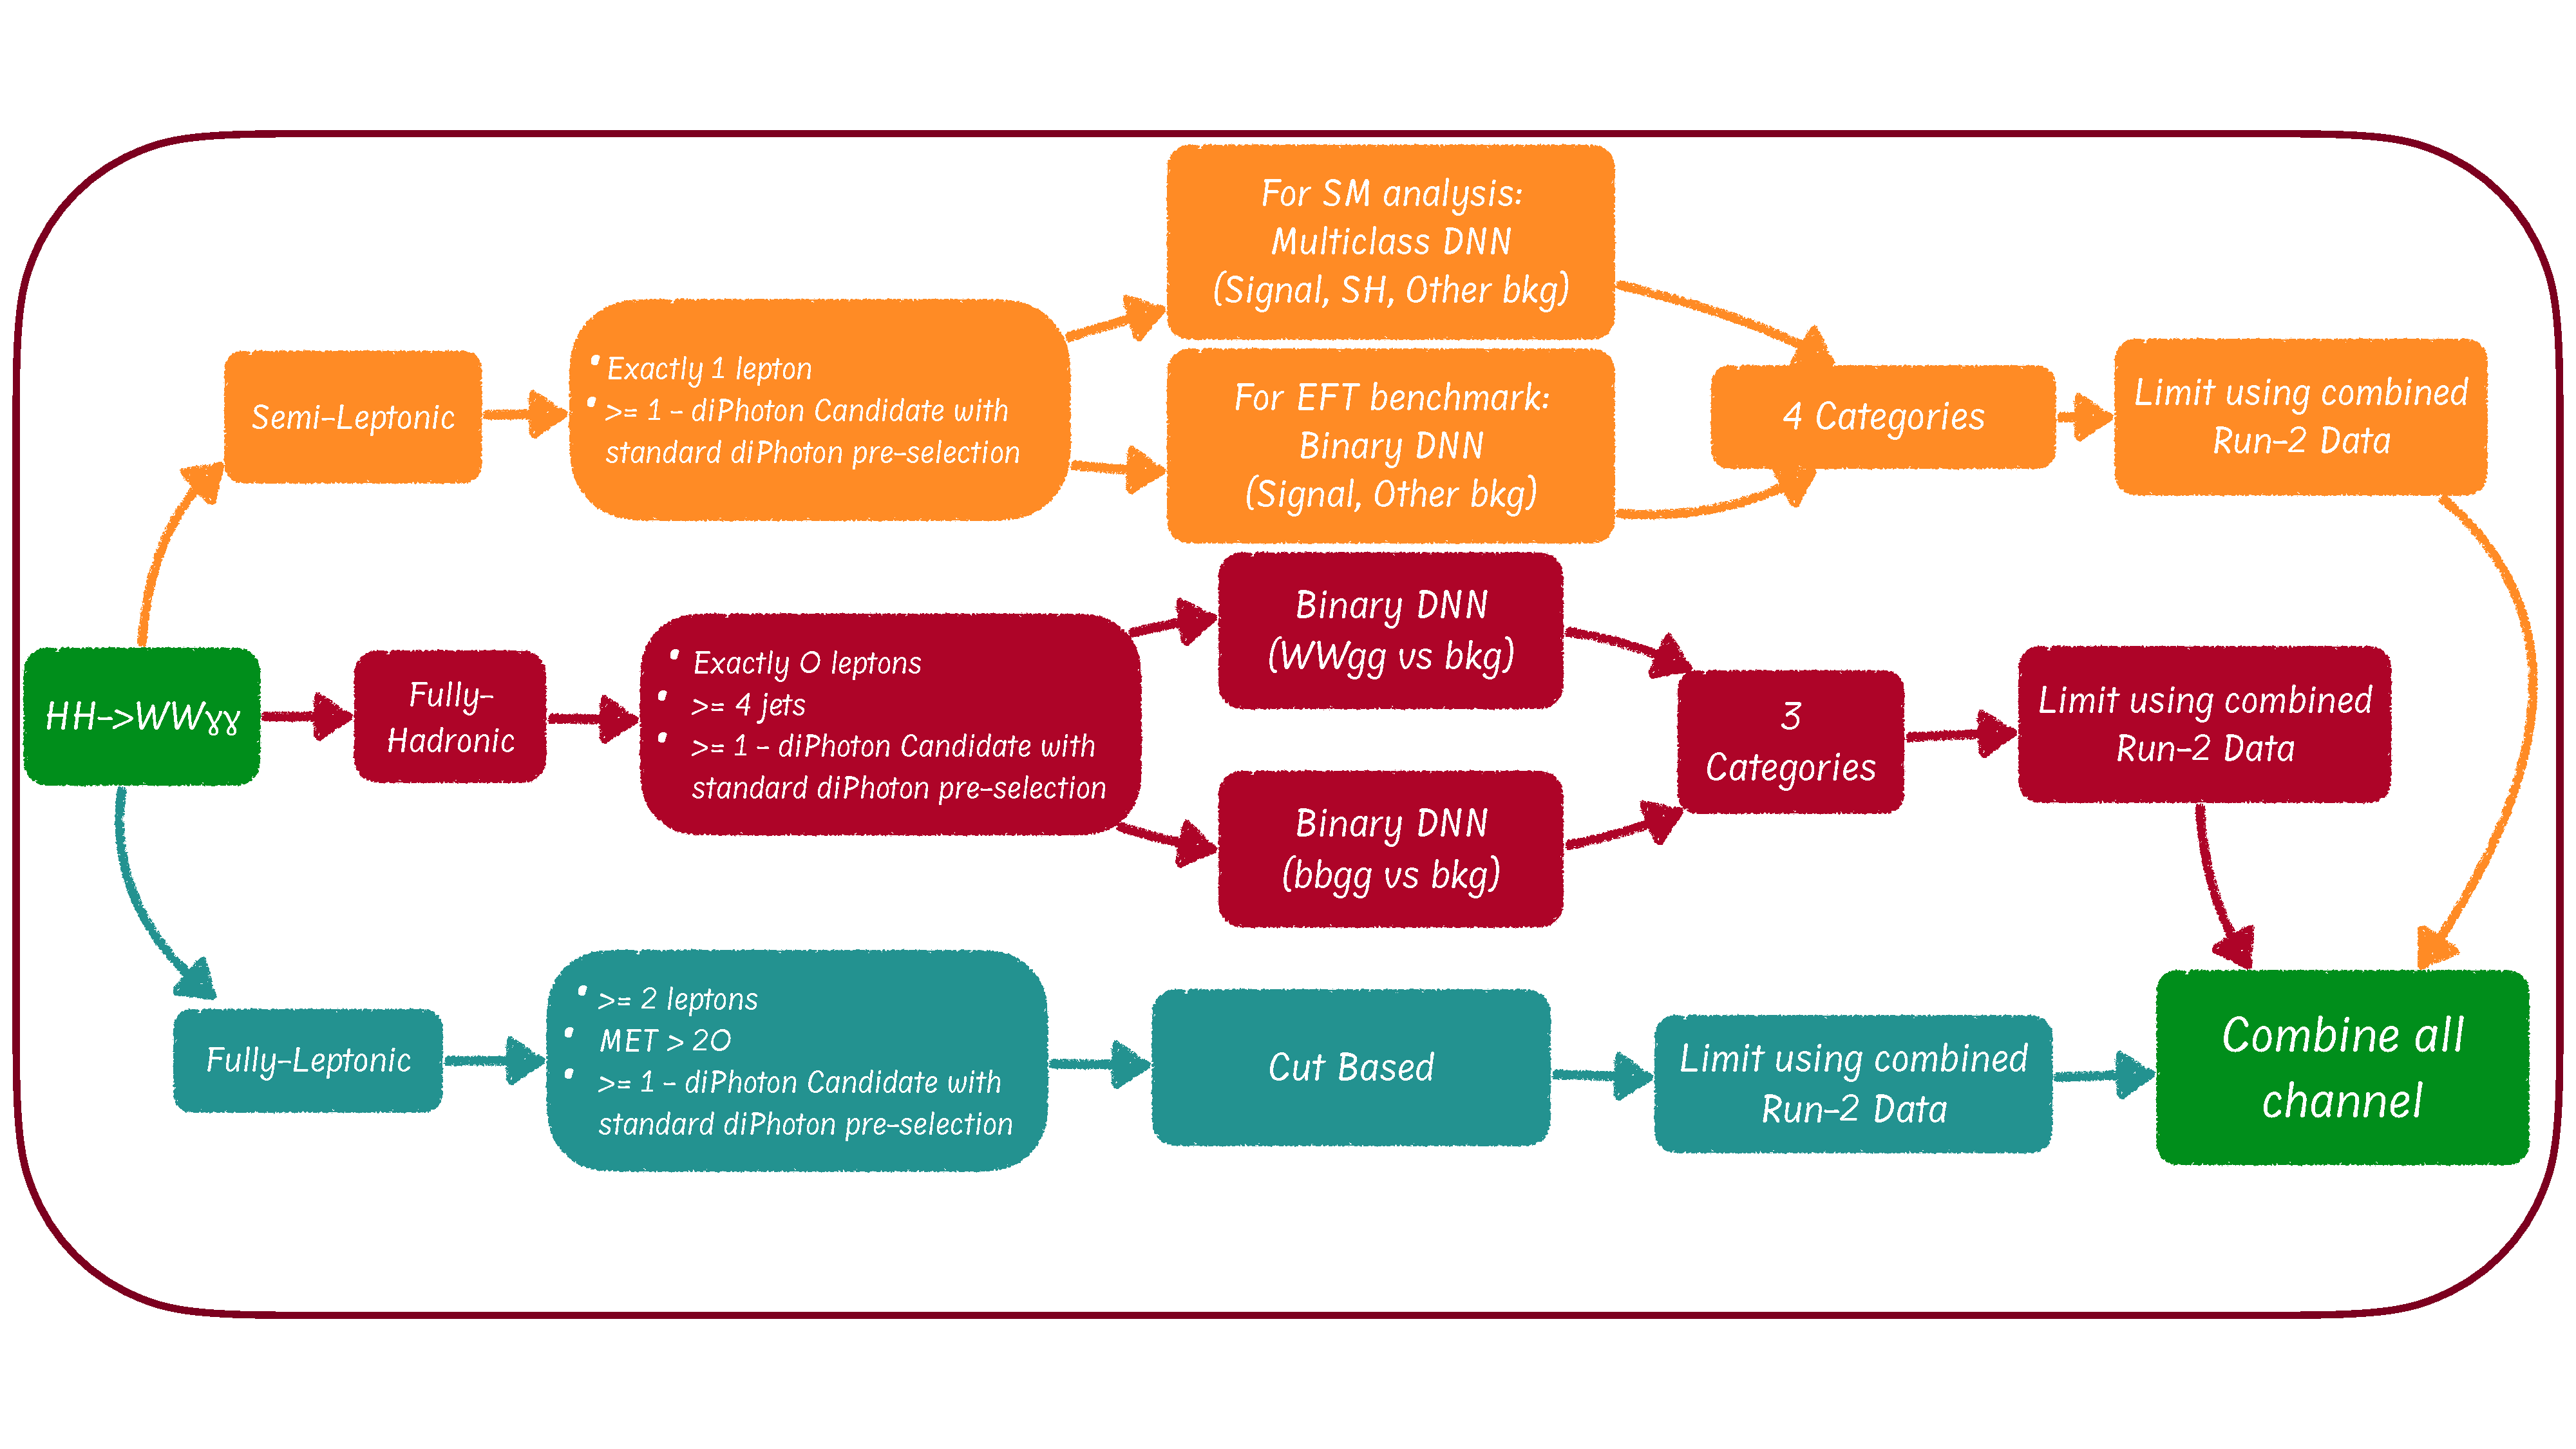
\includegraphics[width=\textwidth,trim={0 3cm 0 3cm},clip=true]{Sections/HHWWgg/images/Strategy/HH_flowchart.pdf}
    \caption{$HH\rightarrow WW\gamma\gamma$ Analysis flow chart}
    \label{fig:HHflowChart}
\end{figure}

Signal and background models are constructed independently for each year of data and MC (2016, 2017 and 2018) and combined to produce signal and background models to fit to the LHC Run 2 dataset. Results are obtained by performing a simultaneous
likelihood fit to the invariant diphoton distribution, \mgg, among all categories. This procedure is performed in order to extract 95\% CL upper limits on di-Higgs production within the context of the SM interpretation. Additionally, through the use of an EFT lagrangian, various simulation templates are fit to data and a linear combination of EFT samples results in the scan of two EFT parameters, and upper limits are extracted on 20 EFT benchmark scenarios. 
\clearpage
\section{EFT description} \label{sec:EFT_Description}

As di-Higgs in the WW$\gamma\gamma$ final state is predicted in the SM, a search for its SM signature is performed. In order to increase the breadth of the search, the analysis is extended to a search for a variety of EFT scenarios predicting the HH$\rightarrow$WW$\gamma\gamma$ process with varying cross sections. This extension branches from the SM, where the Higgs potential before spontaneous symmetry breaking reads as shown in Equation \ref{eq:SM_H_Potential}, where $\Phi$ is an $SU(2)$ doublet scalar field, and $\phi$ is the real part of its neutral component, equal to $v + H$, where $v$ is the field's vacuum expectation value.

\begin{eqnarray} \label{eq:SM_H_Potential}
  V(\Phi) = - \frac{\mu^2}{2}\left|\Phi \right|^2
  +\frac{\lambda}{4} \left|\Phi \right|^4
\end{eqnarray}

Requiring there be a minimum value of this potential leads to the relations shown in Equation \ref{eq:Minimum_relations}.

\begin{eqnarray} \label{eq:Minimum_relations}
  \lambda = \frac{m_H^2}{2 v^2}, \;\;  \mu^2 = \frac{m_H^2}{2},
  \;\; m_H^2 = \frac{\partial^2 V}{\partial \phi^2}
   \label{eqm-2}
\end{eqnarray}

These relations include a determination of the structure of the Higgs self-coupling, $\lambda$, as a value depending on the Higgs mass $m_{H}$ and Higgs vacuum expectation value (VEV) $v$. After spontaneous symmetry breaking, the leading terms of the Higgs potential look as shown in Equation \ref{eq:HiggsPotential_after_SSB}. 

\begin{eqnarray} \label{eq:HiggsPotential_after_SSB}
  V = \frac{m_H^2}{2}H^2 + \lambda_3 v H^3 + \frac{\lambda_4}{4} H^4,
\quad
 \lambda_3 = \lambda_4 = \lambda_{HHH} = \frac{m_H^2}{2v^2}
\end{eqnarray}

Experimentally measuring $\lambda_{HHH}$ is a crucial test of the SM electroweak symmetry breaking mechanism, in order to compare the experimentally measured value to its SM predictions. Modifications of the Higgs self-coupling coupling ($\lambda_{HHH}$) can only be directly accessed via Higgs pair production, making this analysis a good use-case to search for possible BSM effects on the structure of the Higgs self-coupling. 

In this analysis, the effective Lagrangian \cite{deFlorian:2016spz, Carvalho:2015ttv} used to describe Higgs pair production is shown in Equation \ref{Eq:LagrangianBSM}, with its parameters' mathematical definitions shown in Equation \ref{Eq:LagrangianBSM_params}, and corresponding SM and BSM Feynman diagrams shown in Figure \ref{fig:ggHH_production}.

\begin{equation} \label{Eq:LagrangianBSM}
    \mathcal{L}_{BSM} = -{\textcolor{ForestGreen}{\kappa_{\lambda}}} \lambda^{SM}_{HHH} v H^3 -
      \frac{m_t}{v}({\textcolor{blue}{\kappa_t}} H + \frac{\textcolor{red}{c_2}}{v} H^2)(\bar{t_L}t_R + h.c.)
      + \frac{\alpha_S}{12 \pi v}(\textcolor{red}{c_g} H
      - \frac{\textcolor{red}{c_{2g}}}{2 v}H^2)G^a_{\mu \nu}G^{a, \, \mu \nu}
\end{equation}

\begin{eqnarray}\label{Eq:LagrangianBSM_params}
    &&{\textcolor{ForestGreen}{\kappa_{\lambda}}} = \frac{\lambda_{HHH}}{\lambda_{HHH}^{SM}}, \;
    \lambda_{HHH}^{SM} = \frac{ m^2_{H}}{2v^2}, \;\;
    {\textcolor{blue}{\kappa_{t}}} = \frac{ y_{t}}{y_{t}^{SM}}, \;\;
    y_{t}^{SM} = \frac{\sqrt{2} m^2_{t}}{ v}
\end{eqnarray}

\begin{figure}[!htbp]
  \subfloat[SM-like processes]{%
  \label{SMLO_ggHH_production}
            \begin{minipage}[t]{\linewidth}
                  \begin{center}
                          \raisebox{-0.7\height}{ 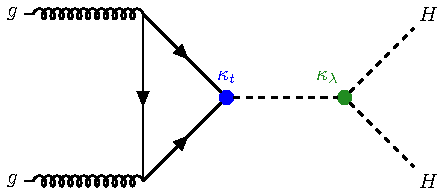
\includegraphics[width=0.45\textwidth]{Sections/HHWWgg/images/EFT_Description/fey_HH_Triangle.pdf} }
                          \raisebox{-0.625\height}{ 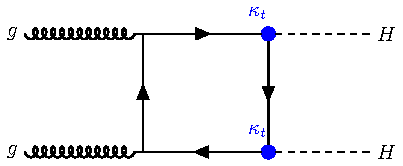
\includegraphics[width=0.45\textwidth]{Sections/HHWWgg/images/EFT_Description/fey_HH_Box.pdf} }
                  \end{center} 
          \end{minipage}%
  }
  
  \subfloat[Pure BSM processes]{%
  \label{BSMLO_ggHH_production}
          \begin{minipage}[t]{\linewidth}
                  \begin{center}
                          \raisebox{-0.7\height}{ 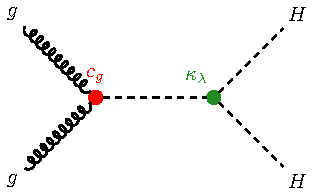
\includegraphics[width=0.30\linewidth,clip]{Sections/HHWWgg/images/EFT_Description/fey_HH_anomal_2_colored.pdf} }
                          \raisebox{-0.7\height}{ 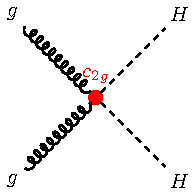
\includegraphics[width=0.20\linewidth,clip]{Sections/HHWWgg/images/EFT_Description/fey_HH_anomal_3_colored.pdf} }
                          \raisebox{-0.7\height}{ 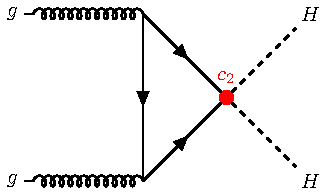
\includegraphics[width=0.30\linewidth,clip]{Sections/HHWWgg/images/EFT_Description/fey_HH_anomal_4_colored.pdf} }
                  \end{center}
          \end{minipage}
  }
  \caption{Feynman diagrams for leading-order Higgs boson pair production via gluon fusion}
  \label{fig:ggHH_production}
  \end{figure}
  

Qualitatively, each of these variables are defined as follows:

\begin{itemize} \label{EFT_parameters_description}
  \item $G^a_{\mu \nu} = \partial_{\mu} G_{\nu}^a - \partial_{\nu} G_{\mu}^a + f^{abc}  G_{\mu}^b G_{\nu}^c$ is the gluon field strength tensor.
  \item $f^{abc}$ is the totally anti-symmetric $SU(3)$ structure tensor.
  \item \textcolor{ForestGreen}{$\kappa_{\lambda}$} is a measure of the deviation of the Higgs boson self-coupling from its SM expectation $\lambda_{HHH}^{SM}$. For example, \textcolor{ForestGreen}{$\kappa_{\lambda}$} = 2 corresponds to a self-coupling with twice the strength as the SM expectation.
  \item \textcolor{blue}{$\kappa_{t}$} is a measure of the deviation of the coupling of a single Higgs boson and two top quarks, called the top Yukawa coupling, from its SM expectation $y_{t}^{SM}$. For example, \textcolor{blue}{$\kappa_{t}$} = 2 corresponds to a top Yukawa coupling with twice the strength as the SM expectation.
  \item \textcolor{red}{$c_{2}$} is the strength of a purely BSM coupling between two Higgs bosons and two top quarks. In the SM this coupling strength equals zero, as the dimension of this added lagrangian term would be non-renormalizable.
  \item \textcolor{red}{$c_{g}$} is the strength of a purely BSM coupling between one Higgs boson and two gluons. In the SM this coupling strength equals zero, corresponding to the fact that gluons are massless in the SM.
  \item \textcolor{red}{$c_{2g}$} is the strength of a purely BSM coupling between two Higgs bosons and two gluons. In the SM this coupling strength equals zero, corresponding to the fact that gluons are massless in the SM.
\end{itemize}

In order to simplify the search of HH models across the entire 5-dimensional phase space and avoid the need to generate simulated events for a large number of points in the 5-dimensional EFT space, a reweighting technique is employed, a set of benchmark EFT points is searched for, and scans of multiple EFT parameters are performed. Within this lagrangian formalization, the differential cross section of of gluon-gluon fusion induced Higgs boson pair production, $\sigma_{HH}$, can be expressed as a polynomial in terms of the EFT model parameters using generator-level information on the HH system as shown in Equation \ref{eq:reweight_eq}.

\begin{equation} \label{eq:reweight_eq}
  \frac{d^2\sigma}{d m_{HH}d|\cos{\theta^*}| } = \sum A_i( m_{HH}, |\cos{\theta^*}| ) \, c_i
\end{equation}

where $c_i$ represents the combinations of couplings defined in \cite{Buchalla:2018yce}, and $A_i( m_{HH}, |\cos{\theta^*}| )$ are known coefficient values. Equation \ref{eq:reweight_eq} is used to extract per event weights, which are normalized by equation \ref{eq:LONLONorm}, where $\sigma_i$ ($\sigma_f$) is the cross section of the initial (final) benchmark point when reweighting i $\rightarrow$ f. This allows one to reweight any HH sample at NLO to any other HH sample at NLO precision. In this analysis, this is used to reweight from a set of generated HH samples at NLO to any point in the 5-dimensional EFT phase space \cite{Carvalho:2016rys,Buchalla:2018yce}. Additionally, when performing DNN trainings in the SL and FH final states, signal samples generated at LO are reweighted to the SM at NLO using this technique in order to provide a larger number of signal events for training.

\begin{equation} \label{eq:LONLONorm}
  w(m_{HH}, |\cos{\theta^*}|) = \frac{d\sigma_f(m_{HH}, |\cos{\theta^*}|)}{d\sigma_i(m_{HH}, |\cos{\theta^*}|)} \cdot \frac{\sigma_i}{\sigma_f}
\end{equation}

With this technique, twenty benchmark scenarios considered in this analysis, chosen as they are largely representative of different kinematic regions of the 5-dimensional EFT phase space \cite{Carvalho:2015ttv,Buchalla:2018yce,Capozi:2019xsi}, are produced via a reweighting of four generated simulation samples at NLO ($\kappa_{\lambda}$ = [0, 1, 2.45, 5]) and are shown in Table \ref{tab:eft_bench}.  

In addition, by considering a linear combination of the four generated simulation samples weighted to their corresponding contribution to arbitrary $\kappa_{\lambda}$ and $c_{2}$ signal hypotheses, scans of these two parameters can be performed in order to constrain their values. The $\kappa_{\lambda}$ parameter also affects the Higgs boson branching ratios and the single Higgs production cross sections because of next-to-leading (NLO) electroweak corrections \cite{Degrassi:2016wml,Maltoni:2017ims}, taken into account when scanning over $\kappa_{\lambda}$ values.

\begin{table}[h]
  \begin{center}
    \begin{tabular}{r|ccccc}
      Benchmark & $\kappa_{\lambda}$ & $\kappa_{t}$ & $c_{2}$	& $c_{g}$ & $c_{2g}$ \\ \hline
      SM &	1.0 & 1.0	 &	0.0		& 0.0	& 0.0 \\ \hline
      1 &	7.5	 & 1.0	 &	-1.0	& 0.0	& 0.0 \\
      2 &	1.0	 & 1.0	 &	0.5		& -0.8	& 0.6 \\
      3 &	1.0	 & 1.0	 &	-1.5	& 0.0	& -0.8 \\
      4 &	-3.5 & 1.5  &	-3.0	& 0.0	& 0.0 \\
      5 &	1.0	 & 1.0	 &	0.0		& 0.8	& -1 \\
      6 &	2.4	 & 1.0	 &	0.0		& 0.2	& -0.2 \\
      7 &	5.0	 & 1.0	 &	0.0		& 0.2	& -0.2 \\
      8 &	15.0 & 1.0	 &	0.0		& -1	& 1 \\
      9 &	1.0	 & 1.0	 &	1.0		& -0.6	& 0.6 \\
      10 &	10.0 & 1.5   &	-1.0	& 0.0	& 0.0 \\
      11 &	2.4	 & 1.0	 &	0.0		& 1		& -1 \\
      12 &	15.0 & 1.0	 &	1.0		& 0.0	& 0.0 \\[0.5ex] \hline 
      8a &  1.0  & 1.0   &  0.5   & $\frac{0.8}{3}$ & 0.0 \\[0.5ex] 
      1b &  3.94 & 0.94  & $\frac{-1}{3}$ & 0.75 & -1 \\[0.5ex] 
      2b &   6.84 & 0.61 &  $\frac{1}{3}$ &  0.0 & 1.0 \\[0.5ex] 
      3b &   2.21 & 1.05 & $\frac{-1}{3}$ &  0.75 &  -1.5 \\[0.5ex] 
      4b &   2.79 & 0.61 &  $\frac{1}{3}$ & -0.75 &  -0.5 \\[0.5ex] 
      5b &   3.95 & 1.17 & $\frac{-1}{3}$ & 0.25 &  1.5 \\[0.5ex] 
      6b &   5.68 & 0.83 &  $\frac{1}{3}$ & -0.75 &  -1.0 \\[0.5ex] 
      7b &   -0.10 & 0.94 &         1.0 & 0.25 & 0.5 \\
    \end{tabular}
  \end{center}
  \caption{Parameter values of the 20 EFT benchmarks and the Standard Model. \label{tab:eft_bench}}
\end{table}

\clearpage 
\section{Samples} \label{sec:samples}

In order to perform the analysis, datasets collected with the CMS detector from 2016-18 are used, as well as a slew of simulation samples in order to optimize the analysis strategy for the desired HH$\rightarrow$WW$\gamma\gamma$ physics signature, and perform statistical inferences by fitting simulation to data in order to extract the analysis' final results. 

In this Section, the CMS data samples used will be described in Section \ref{sec:data_samples}, the simulated signal samples will be described in Section \ref{sec:signal_simulation}, the simulated background samples will be described in Section \ref{sec:background_simulation}, and the corresponding simulation hadronization and detector response will be described in Section \ref{sec:HadronizationAndDetectorResponse}. 

\subsection{Data} \label{sec:data_samples}

The analyzed data correspond to a total integrated luminosity of 138 \unit{fb$^{-1}$} and were collected during Run 2 at the LHC from 2016 to 2018. In order to select events which may come from the HH$\rightarrow$WW$\gamma\gamma$ process, events with highly energetic photons are selected in order to tag the H$\rightarrow\gamma\gamma$ leg of the HH process.

Events are selected using double-photon triggers with thresholds on the leading (subleading) photon transverse momentum (\pt) of $p_T^{\gamma} > 30 \ (18)$ GeV
for the data collected during 2016
and $p_T^{\gamma} > 30 \ (22)$ GeV for 2017 and 2018.
In addition, loose calorimetric identification requirements \cite{Sirunyan:2018ouh}, based
on the shape of the electromagnetic shower, the isolation of the photon candidate, and the ratio
between the hadronic and electromagnetic energy deposit of the shower, are imposed on the
photon candidates at the trigger level.

The HLT paths applied to events from these datasets are:

\begin{center}
        {\tt HLT\_Diphoton30\_18\_R9Id\_OR\_IsoCaloId\-\_AND\_HE\_R9Id\_Mass90} (2016 data) \\ 
        {\tt HLT\_Diphoton30\_22\_R9Id\_OR\_IsoCaloId\-\_AND\_HE\_R9Id\_Mass90} (2017 and 2018 data) \\
        {\tt HLT\_Diphoton30\_22\_R9Id\_OR\_IsoCaloId\-\_AND\_HE\_R9Id\_Mass95} (2017 and 2018 data) \\ 
\end{center}

Datasets expected to contain events with two photons are used in order to obtain events containing the $H\rightarrow\gamma\gamma$ process,
and further selections are applied to identify events that also contain the $H\rightarrow WW$ process. 

\subsection{Signal simulation} \label{sec:signal_simulation}

% SIGNAL
Di-Higgs signal Monte-Carlo (simulation) samples in the gluon-gluon fusion production mode are generated using POWHEG v2 \cite{Nason:2004rx, Frixione:2007vw, Alioli:2010xd, Heinrich:2019bkc}
at NLO in QCD including the full top quark mass dependence
for four different sets of $(\kappa_{\lambda}, \kappa_{t})$ parameter values: $(1, 1)$, $(2.45, 1)$, $(5, 1)$ and $(0, 1)$, where these parameters are defined in section \ref{EFT_parameters_description}. 
In addition, 12 EFT benchmark samples in a five-dimensional EFT model space are generated at LO \cite{Carvalho:2015ttv} using MadGraph, where the EFT coupling parameter values are defined in the rows labelled 
1-12 of Tab. \ref{tab:eft_bench}.   

A combination of the four NLO signal simulation samples, in which the EFT parameters are varied as $(\kappa_{\lambda}, \kappa_{t}) = $ $(1, 1)$, $(2.45, 1)$, $(5, 1)$ and $(0, 1)$, is reweighted using an analytic formula derived in \cite{Carvalho:2016rys,Buchalla:2018yce}. The analytic formula is shown in Eq.\ref{eq:reweight_eq}. 
The signal hypotheses to which this combination of NLO samples is reweighted to are defined as the 20 benchmark scenarios (1-12 \cite{Carvalho:2015ttv}, 8a \cite{Buchalla:2018yce}, 1b-7b \cite{Capozi:2019xsi}), shown in Tab. \ref{tab:eft_bench}. 

A possible way to improve this analysis in the future would be to include the VBF production mode of HH in the signal definition, and include a dedicated VBF tagging category in order to improve the overall analysis sensitivity. While this may not have a significant impact on the final result due to its low production cross section, it may be able to improve the sensitivity of the analysis on order of $\approx$ 5\%. 

\subsection{Background simulation} \label{sec:background_simulation}

% add feynman diagrams?

% BACKGROUNDS
The analysis is affected by backgrounds from single Higgs boson production and by non-resonant backgrounds which manifest as a continuum in the $m_{\gamma\gamma}$ spectrum.
Monte Carlo event generators were used for the simulation of the background from SM single Higgs boson production, including
gluon gluon fusion ($ggH$), associated production with a $Z$ or $W$ boson ($VH$), associated production with a top quark pair ($ttH$)
simulated at NLO in QCD precision using MadGraph5\_aMCatNLO \cite{Alwall:2014hca, Artoisenet:2012st} with the FxFx merging scheme \cite{Frederix:2012ps},
and vector-boson fusion (VBF $H$) using POWHEG v2 \cite{Nason:2004rx, Frixione:2007vw}.

The continuum background contribution from SM processes with multiple photons is estimated using data-driven methods described in Sec. \ref{sec:AnalyticFitting_Background}. In the SL and 
FH final states, MVA methods are employed which use background MC for training.
The continuum background MC includes $\gamma+$jets modeled with the PYTHIA 8 \cite{Sjostrand:2014zea} generator, $\gamma\gamma+$jets modeled with the SHERPA v.2.2.1 generator \cite{Bothmann:2019yzt}, $0,1,2\gamma+W+$jets, $t\bar{t}$, and $t\bar{t}W$ modeled using MadGraph5\_aMCatNLO \cite{Alwall:2014hca,Artoisenet:2012st,Frederix:2012ps}.

% \subsection{MC}

% The analysis is affected by backgrounds from single-Higgs-boson production and by non-resonant backgrounds with continuum $m_{\gamma\gamma}$ spectra.
% The continuum background contribution from SM processes with multiple photons and jets is estimated using data-driven methods described in Sec. \ref{sec:AnalyticFitting_Background}. 
% Monte Carlo event generators were used for the simulation of the background from SM single Higgs boson production, including 
% gluon–gluon fusion ($ggH$), associated production with a Z or W boson ($VH$), associated
% production with a top quark pair ($ttH$) and vector-boson fusion (VBF H) (Table \ref{tab:SMH_MCMiniAODSamples}). 

% In addition, the DNN based analyses in the Semi-Leptonic channel uses the 2017 background MC MiniAOD samples in Table \ref{tab:MCMiniAODSamples} and Table \ref{tab:SMH_MCMiniAODSamples} for training.

% \subsection{Signal MC}
% In the Effective Field Theory (EFT) description, gluon-gluon fusion Higgs boson pair production can be generally described by five parameters ($\kappa_{\lambda}$, $\kappa_{t}$, $c_{2}$, $c_{g}$, $c_{2g}$) controlling the tree-level interactions 
% of the Higgs boson as described in Ref \ref{section:introduction}, and shown in Figure \ref{fig:ggHH_production}.
% For the experimental exploration of the five-dimensional EFT model space, 12 benchmarks (Table \ref{tab:eft_bench}) are considered following \cite{Carvalho:2016rys, Carvalho:2015ttv}.
% This manageably small set of benchmark points can be used to represent the volume of the unexplored parameter space.

% The LO EFT MC samples generated using the full CMS detector simulation are listed in Table \ref{tab:eft_samples}. 
% The generation is performed with MadGraph5\_aMCatNLO \cite{Alwall:2014hca}.
% Unfortunatly, when the simulation was launched within the CMS system, the version of the EFT benchmarks was preliminary, meaning the simulated 
% samples used an outdated version of the recommended benchmarks. 
% In addition, for 2017 and 2018 MC production, a mistake was made during the production of the SM sample, where the value of the $c_g$ coupling was set to 1.0.
% % Is this also true for all of the other benchmarks? I thought this was the case but perhaps I am remembering incorrectly.

% In order to use the updated clustering scheme with the 12 BSM benchmarks and SM point, a reweighting is implemented to obtain the benchmarks of interest.
% The reweighting procedure used is described in Section \ref{sec:reweighting}.

% %% I think we should add Feynman Diagrams to show the different EFT couplings. Maybe the SM diagrams can be added to the introduction.  
% \begin{table}[h]
%   \begin{center}
%     \begin{tabular}{r|ccccc}
%       Benchmark & $\kappa_{\lambda}$ & $\kappa_{t}$ & $c_{2}$	& $c_{g}$ & $c_{2g}$ \\ \hline \\
%       1 &	7.5	 & 1.0	 &	-1.0	& 0.0	& 0.0 \\
%       2 &	1.0	 & 1.0	 &	0.5		& -0.8	& 0.6 \\
%       3 &	1.0	 & 1.0	 &	-1.5	& 0.0	& -0.8 \\
%       4 &	-3.5 & 1.5  &	-3.0	& 0.0	& 0.0 \\
%       5 &	1.0	 & 1.0	 &	0.0		& 0.8	& -1 \\
%       6 &	2.4	 & 1.0	 &	0.0		& 0.2	& -0.2 \\
%       7 &	5.0	 & 1.0	 &	0.0		& 0.2	& -0.2 \\
%       8 &	15.0 & 1.0	 &	0.0		& -1	& 1 \\
%       9 &	1.0	 & 1.0	 &	1.0		& -0.6	& 0.6 \\
%       10 &	10.0 & 1.5   &	-1.0	& 0.0	& 0.0 \\
%       11 &	2.4	 & 1.0	 &	0.0		& 1		& -1 \\
%       12 &	15.0 & 1.0	 &	1.0		& 0.0	& 0.0 \\ \hline
%       SM &	1.0 & 1.0	 &	0.0		& 0.0	& 0.0 \\
%       Box &	0.0 & 1.0	 &	0.0		& 0.0	& 0.0 \\
%     \end{tabular}
%   \end{center}
%   \caption{Parameter values of the twelve benchmarks and the Standard Model and Box points. \label{tab:eft_bench}}
% \end{table}

% In addition, NLO in QCD MC samples are generated using Powheg \cite{Nason:2004rx, Frixione:2007vw, Alioli:2010xd, Heinrich:2019bkc} for four different sets of $(\kappa_{\lambda}, \kappa_{t})$ parameters: $(1, 1)$, $(2.45, 1)$, $(5, 1)$ and $(0, 1)$. The NLO samples are listed in Table \ref{tab:eft_nlo_samples}. 

% The PYTHIA 8 \cite{Sjostrand:2014zea} package is used for parton showering, hadronization, and the underlying event simulation of LO and NLO signal samples, 
% with parameters set by the CUETP8M1 tune \cite{Khachatryan:2015pea} (2016 data taking period) and the CP5 tune \cite{Sirunyan:2019dfx} (2017 and 2018 data taking periods). The signal samples are generated for the three possible final states of $WW$ system: Semi-Leptonic ($WW\rightarrow qql\nu$), Fully-Leptonic ($WW\rightarrow l\nu l\nu$) and Fully-Hadronic ($WW\rightarrow qqqq$) where $l = e, \mu$ or $\tau$.
% Signal samples are also generated for the Fully-Hadronic $ZZ$ final state: $ZZ \rightarrow qqqq$.  

\subsection{Hadronization and detector response} \label{sec:HadronizationAndDetectorResponse}

% HADRONISATON & DETECTOR RESPONSE
The PYTHIA 8 \cite{Sjostrand:2014zea} package is used for parton showering, hadronization, and the underlying event simulation of all signal and background samples (with the exception of $1,2\gamma+$jets MC from SHERPA v.2.2.1),
with parameters set by the CUETP8M1 tune \cite{Khachatryan:2015pea} (2016 data taking period) and the CP5 tune \cite{Sirunyan:2019dfx} (2017 and 2018 data taking periods). Parton distribution functions (PDFs) are taken from the NNPDF3.0 set \cite{Ball:2014uwa}.
The response of the CMS detector is modeled using the Geant4 package \cite{AGOSTINELLI2003250}.
The simulated events include additional $pp$ interactions within the same or nearby bunch crossings (pileup), generated using Pythia and overlaid on the MC events using event weights so that the distribution of the number of collisions matches the data.

\clearpage
\section{Objects} \label{sec:Objects}

When processing the CMS data and simulated physics samples described in Section \ref{sec:samples}, a particle flow (PF) \cite{CMS:2017yfk} algorithm is used in order to define objects from real or simulated CMS detector information. Objects corresponding to the following particles are utilized in the analysis: Photons, electrons, muons, and ``jets'' resulting from hadronized quarks or gluons. In addition, a special object called ``MET'' (Missing transverse momentum) is utilized in order to tag events which may contain particles which evade detection such as neutrinos. 

The same object definitions are used for all WW$\gamma\gamma$ final state categories when reconstructing objects from both data and simulation events.

In this section, the choice and reconstruction of the following objects is described: Vertex choice in Section \ref{sec:vertex}, photons in Section \ref{sec:photons}, electron and muons in Section \ref{sec:LeptonSelections}, jets in Section \ref{sec:Jets} and MET in Section \ref{sec:MET}. Finally, the yields and efficiencies of the signal and background processes in this analysis after the selections described in this section are described in Section \ref{sec:Preselection_yields}.

\subsection{Vertex} \label{sec:vertex}

Because there can be many simultaneous interactions in a given CMS event due to the large number of protons in colliding LHC protons bunches, many interactions points may be reconstructed. In order to identify the vertex corresponding to the highest energy interaction of the proton-proton collisions, called the ``hard interaction'', the vertex which has the highest sum of $p_{T}^{2}$ is chosen as the point from which photons are reconstructed and from which jets are taken. This is chosen as in the WW$\gamma\gamma$ processes, high $p_{T}$ tracks from the WW decay products are expected, namely from leptons and jets.

In Figure \ref{fig:VtxEff}, the probability of choosing a vertex with a z-position along the colliding axis within $|dZ|$ of the z-position of the generator level vertex is shown for the 2017 SM at NLO semi-leptonic signal sample. It is shown from the first few points
that the selected reconstructed vertex has an absolute z position within 0.1cm of the z position of the generator vertex for more than 99\% of events. This indicates that the choice of the vertex with the highest sum of $p_{T}^{2}$ is an appropriate choice for the HH$\rightarrow$WW$\gamma\gamma$ process. 

\begin{figure}[H]
    \centering
    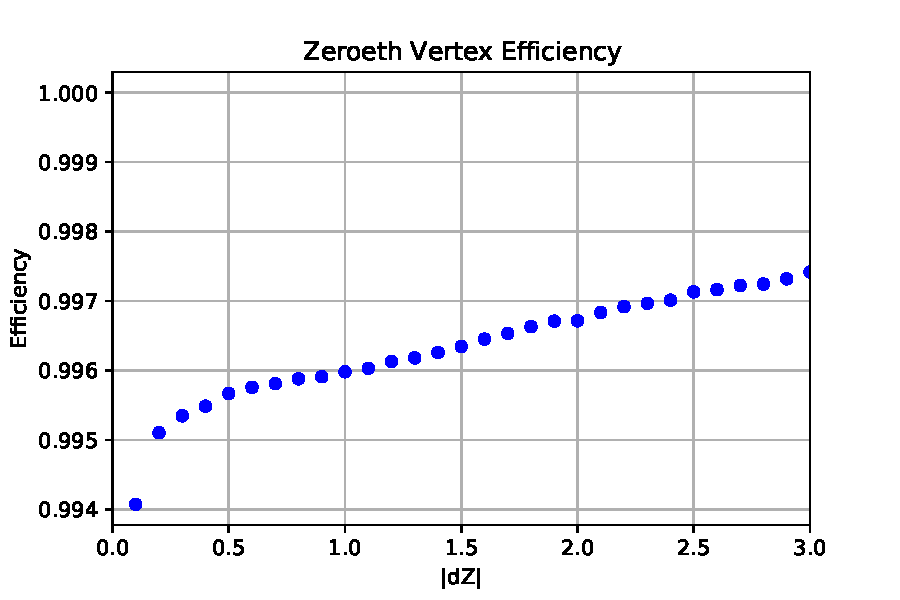
\includegraphics[width=0.75\textwidth]{Sections/HHWWgg/images/Objects/VtxEff.pdf}
    \caption{Efficiency vs $|dZ|$ for the Semi-Leptonic Signal}
\label{fig:VtxEff}
\end{figure}

\subsection{Photons} \label{sec:photons}

Photons used in this analysis are selected from the PF set of photon candidates.
The energy of each photon candidate is estimated from the Supercluster (SC), which
includes deposits from the many particles comprising the electromagnetic shower. In
some cases, photons will interact with detector material upstream of the ECAL and
produce an electron-positron pair; these are known as ``converted'' photons. Converted
photons will also deposit energy in the ECAL preshower detector (ES), which is included
in the SC energy estimate. A correction is then made to this SC energy using a
multivariate regression technique~\cite{Sirunyan:2018ouh}. After that, data and MC are brought into agreement
by applying additional scale and smearing corrections to the photon energies. Once the
photon energy has been established, a set of preselection criteria is applied to obtain the
final set of photons considered in the analysis. One of these criteria is a requirement
placed on the output score of the photon identification BDT, which is trained to
reduce the contamination from other objects which mimic real photons. 

All data events are required to have fired the high-level trigger (HLT) double photon paths and pass diphoton preselections. Simulated events are only required to pass diphoton preselections, defined to be tighter than the HLT dataset requirements. 

The HLT trigger paths used in this analysis are defined in Section \ref{sec:data_samples}, and require the presence of two isolated photons with one photon \pt higher than 30 GeV and the other one with a \pt of at least 18 GeV for 2016 or 22 GeV for 2017 and 2018 in order to keep the bandwidth of the HLT at sustainable levels. The trigger efficiency of each year is measured using data collected at the LHC by CMS and is applied to simulation samples. Higgs candidates with diphoton decays are then built from pairs of photon candidates.

Photon candidates are subject to a pre-selection that imposes requirements on photon kinematics, hadronic leakage, and shower shape. The pre-selection is designed to be slightly more stringent than the trigger requirements, where the pre-selection cuts are summarized in Table~\ref{tab:preselection}. 
The shower shape and isolation variables in simulation are corrected with
a chained quantile regression method~\cite{DBLP:journals/corr/abs-1211-6581}
based on studies of \Ztoee events.
Each variable is corrected with a separately trained boosted decision tree (BDT),
taking the photon kinematic properties, per-event energy density, and the previously corrected features as inputs to ensure that correlations between the inputs are preserved and closer to those in data.
This correction method also improves the modeling of the photon identification (photon ID)
discriminant in MC simulation with respect to the previous CMS~\Htogg results~\cite{Sirunyan:2018ouh}.
A multivariate identification method, based on photon shower-shape, isoaltion and kinematic variables, is used to separate \Htogg signal from background photons (photon ID). A very loose requirement on the photon ID score above -0.9 is applied as a further selection, which eliminates a very significant amount of non-prompt photons while keeping almost 100$\%$ of prompt photons.
Each photon candidate is required to satisfy the ``conversion-safe" electron-veto, which aims to reject photon objects which may have been reconstructed from real electrons.

Additionally, both photons must pass either \RNINE$>$ 0.8,
 $Iso_{ch,had}<$ 20 GeV, or $Iso_{ch,had}$/ \pt $<$ 0.3 if their \pt is above 14 GeV and H/E is below 0.15. \RNINE is defined as the energy sum of the 3 × 3 crystal matrix centered on the most energetic
crystal in a given ECAL supercluster, divided by the energy of the supercluster, and H / E represents the ratio of hadronic energy to electromagnetic energy.

\begin{table}[htbp]
        \caption{List of photon preselection requirements.}
        \begin{center}
                \begin{tabular}{|l|l|l|l|l|l|}
                        \hline
                        & H/E     & $\sigma_{i\eta i\eta}$ & \RNINE & $Iso_{ph}$ & $Iso_{track}$ \\
                        \hline
                        EB; R9$>$  0.85   & $<$0.08 & --       & $>$0.5  & -- & --\\
                        \hline
                        EB; R9$\leq$0.85  & $<$0.08 & $<$0.015 & $>$0.5  & $<4.0$ & $<6.0$\\
                        \hline
                        EE; R9$>$0.90     & $<$0.08 & --       & $>$0.8  & -- & --\\
                        \hline
                        EE; R9$\leq$0.90  & $<$0.08 & $<$0.035 & $>$0.8  & $<4.0$ & $<6.0$\\
                        \hline
                \end{tabular}
        \end{center}
        \label{tab:preselection}
\end{table}

Preselection efficiencies and the loose photon ID cut efficiency are determined from data using \Ztoee~ events with the tag and probe method. By definition the tag and probe technique using \Ztoee~ does not allow for the measurement of the electron-veto efficiency, which instead is measured independently using \Ztommg~ events. The scale factors, defined as the ratio of efficiency in data to efficiency in simulation, are used to correct the signal efficiency in simulated signal samples and the uncertainties are propagated to the expected signal yields.

Each event is required to have at least one diphoton candidate constructed with respect to the
zeroth vertex that passes the preselections described above. The largest-\pt photon (leading) is required to have
\pt $>$ 35 GeV and the second largest (subleading) is required to
have  \pt $>$ 25 GeV. These photons must also pass a loose selection on a dedicated $H\rightarrow\gamma\gamma$ photon ID shown in Table \ref{tab:PhotonSelections}.

\begin{table}[htbp]
        \begin{center}
                \begin{tabular}{c|cc}
                         \hline
                         & Leading Photon & Subleading Photon \\ \hline
                         %$\frac{p_{T}}{m_{\gamma\gamma}}$ & (1/3) & (1/4) \\
                         Photon ID & -0.9 & -0.9 \\ \hline
                \end{tabular}
        \end{center}
        \caption{Additional photon object selections}
        \label{tab:PhotonSelections}
\end{table}


Finally, the events with the invariant mass of two photons within $100 < \mgg < 180$ GeV, are selected for the signal extraction.

\subsection{Leptons} \label{sec:LeptonSelections}

In this analysis, electron and muon objects are considered, and the analysis remains agnostic to tau leptons, as they are neither tagged nor rejected. Because the number of leptons is used as a handle of orthogonality between the three final state categories, it is necessary that all final state categories apply the same lepton selections. A possible way to improve this analysis in the future would be to include the tagging of tau leptons, which may be present in the leptonic WW$\gamma\gamma$ final states. 

For electrons and muons, ID MVA outputs are utilized in order to identify leptons with different balances of sensitivity and yields. Additionally, isolation criteria is defined and utilized in order to quantify how isolated leptons are from other objects. The decision of which electron ID, muon ID and muon isolation to select comes from comparing the ratio of signal yields after preselections and subsequent lepton selections for the two final state categories containing leptons: the semi-leptonic and fully-leptonic final states. This figure is checked
when applying a loose cut based electron ID with a tight Muon ID and isolation, versus applying a medium MVA based electron ID with a medium Muon ID and isolation. Comparing the ratios between sets of lepton
selections allows one to observe which categories lose the most signal due to the corresponding lepton selections. The relative yields are shown in Table \ref{tab:LeptonSelectionYields}.

\begin{table}[htbp]
    \begin{center}
            \begin{tabular}{|c|c|c|c|c|c|c|}
                    \hline
                    Category & $SL_{e}$ & $SL_{\mu} $ & $FL_{ee}$ & $FL_{\mu\mu}$ & $FL_{e\mu}$ & $FL_{\mu e}$ \\
                    \hline
                    Loose Electron, Tight Muon   & 0.16 & 0.20 & 0.018  & 0.053 & 0.038 & 0.037  \\
                    \hline
                    Medium Electron, Medium Muon  & 0.023 & 0.228 & 0.0006  & 0.062 & 0.0067 & 0.005 \\
                    \hline
                    Ratio & 0.14375 & 1.14 & 0.0333 & 1.17 & 0.176 & 0.135 \\
                    \hline
            \end{tabular}
    \end{center}
    \caption{Ratio of signal yields after preselections and \pt/\mgg cuts over the addition of lepton requirements, and the ratio between the two pairs of lepton requirements. In this analysis, the selections in the top row are used (Loose electron, tight muon), while the other two rows are produced in order to determine the ideal combination of lepton selections to use. \label{tab:LeptonSelectionYields}}
\end{table}

In the Fully-Hadronic final state category, events are required to contain exactly zero leptons. This means that the choice of lepton selection can impact the FH yields, as it may change whether an event has zero leptons or not. The ratio of FH signal yield between the two sets of lepton IDs and ISOs is found to be
0.947, where about 5\% of signal events are lost when using medium MVA based electron ID and medium Muon ID and ISO.

Exactly one lepton is required to pass selections in the SL (Semi-Leptonic) category, therefore for this check the yields for this process are split into the $SL_{e}$ (Semi-Leptonic electron) and $SL_{\mu}$ (Semi-Leptonic muon)
subcategories. For the FL (Fully-Leptonic) category, it is required that exactly two leptons pass the common set of lepton selections, and therefore for the purpose of this check, this process is split into four sub-categories corresponding to the flavours of the
leading two leptons. 

Applying a medium MVA based electron ID reduced subcategory yields containing electrons by factors of 0.14375, 0.0333, 0.176 and 0.135, while subcategories containing a muon
change by factors of 1.14, 1.17, 0.176 and 0.135. While a slight gain is obtained from loosing the muon ID and isolation, most signal events are rejected from tightening electron ID, especially
in the di-electron FL subcategory whose ratio of selected events to pre-selected events is reduced by a factor of about 30.

Because a DNN method is applied in the Semi-Leptonic final state, it is desirable to use looser selections in order to keep more events to input for training. In the Fully-Leptonic analysis,
as the expected yield is already low, it is desirable to preserve signal while also maintaining enough events in the data sideband regions to perform a data driven background fit. For muon subcategories,
as the yields are not affected drastically by tightening the muon ID and isolation from medium to tight, these selections are determined desirable in order to tag muons with
greater purity.

Therefore, all electrons are required to pass a loose cut based ID, and muons are required to pass a Tight ID and posses a relative PF isolation value in a cone of $\Delta R < 0.4$ less than 0.15, as defined in Eq. \ref{eqn:MuonIsoDef}. This is
required for all three final state categories.

\subsubsection{Electrons}

% https://github.com/cms-analysis/flashgg/blob/4e958a7c7997466be6c95115734527577d9d88d8/MicroAOD/python/flashggLeptonSelectors_cff.py
All PF Electrons considered must pass a group of selections in order to consistitue a high $p_{T}$ electron that may have come from a leptonically decaying W boson.
Each electron is required to pass the selections in Table \ref{tab:ElectronSelections}. Scale factors corresponding to loose cut based electron ID are applied as a multiplicative factor to
the central event weight to account for the discrepancy in data / MC electron ID assignment. 

In addition to a loose electron ID, electron candidates are required to have $p_{T} > $ 10 GeV, and a pseudorapidity in the range (0 $<$ $|\eta|$ $<$ 1.4442) or (1.566 $<$ $|\eta|$ $<$ 2.5) in order to remain in the CMS tracker region and avoid the ECAL overlap region. Furthermore, a distance parameter value ($\Delta R = \sqrt{(\Delta\eta)^{2} + (\Delta\phi)^{2}}$) greater than 
0.4 is required between each electron candidate and each of the two photon candidates from the event's highest $p_{T}$ diphoton in order to select isolated electron candidates. A distance parameter value 
of less than 0.4 is also required between the electron candidate's track and ECAL supercluster position, and a 
distance parameter value with each jet candidate $>$ 0.4 is required. Finally, the invariant mass of the electron with each photon candidate in the event's highest \pt diphoton 
candidate must be at least 5 GeV greater or less than the Z boson mass in order to avoid selecting events coming from Z$\rightarrow$ee decays. 

\begin{table}[H]
    \begin{center}
        \begin{tabular}{c|c}
        Variable & Selection \\ \hline
        $p_{T}$ [GeV] & $>$ 10 \\
        $|\eta|$ & (0 $<$ $|\eta|$ $<$ 1.4442) or (1.566 $<$ $|\eta|$ $<$ 2.5) \\
        ID & Loose Cut Based \\
        $\Delta R(e^{-},\gamma)$ & $>$ 0.4 \\
        $\Delta R(e^{-},jet)$ & $>$ 0.4 \\
        $\Delta R(track_{e^{-}},SC_{e^{-}})$ & $<$ 0.4 \\
        $|m_{e^{-}\gamma}$ - 91.187$|$ [GeV] & $>$ 5
        \end{tabular}
    \end{center}
    \caption{
        Electron object requirements
    }
    \label{tab:ElectronSelections}
\end{table}

\subsubsection{Muons}

Selections are applied to all muon objects with the aim of identifying a muon coming from a leptonically decaying W boson. Each muon object is required to pass
the selections in Table \ref{tab:MuonSelections}. In addition to a tight Muon ID, muon candidates are required to have $p_{T} > $ 10 GeV, a pseudorapidity in the range ($|\eta| < 2.4$) to remain in the CMS tracker region, a distance parameter value with each photon candidate $>$ 0.4, a 
distance parameter value with each jet candidate $>$ 0.4, and an isolation $<$ 0.15, as defined in Eq. \ref{eqn:MuonIsoDef}, in order to select isolated muon candidates, where sumPUPt is the summed transverse momentum of charged particles not from the primary vertex.

\begin{table}[H]
    \begin{center}
        \begin{tabular}{c|c}
        Variable & Selection \\ \hline
        $p_{T}$ [GeV] & $>$ 10 \\
        $|\eta|$ & $<$ 2.4 \\
        ID & Tight \\
        $\Delta R(\mu,\gamma)$ & $>$ 0.4 \\
        $\Delta R(\mu,jet)$ & $>$ 0.4 \\
        $I_{\mu}$ & $<$ 0.15
        \end{tabular}
    \end{center}
    \caption{
        Muon object requirements
    }
    \label{tab:MuonSelections}
\end{table}

Scale factors for each year corresponding to the applied tight muon ID are applied to the event weight for each lepton passing all Muon selections, in order to improve the agreement between data and simulation.

\begin{equation}
   I_{\mu} = \frac{( sumChargedHadronPt + max(0, sumNeutralHadronEt + sumPhotonEt - \frac{sumPUPt}{2}) )}{p^{\mu}_{T}}
   \label{eqn:MuonIsoDef}
\end{equation}
% https://twiki.cern.ch/twiki/bin/view/CMSPublic/SWGuideMuonId %% Muon ID definition
\subsection{Jets} \label{sec:Jets}

Jets are constructed using the anti-$k_{T}$ clustering method with a distance parameter of 0.4, classifying them as ``AK4 jets". The selections applied on jets are
shown in Table \ref{tab:JetSelections}. Jet candidates are 
required to have $p_{T} > $ 25 GeV, an absolute value of pseudorapidity $<$ 2.4, are required to pass a loose PU Jet ID in order to avoid reconstructing
jets from pileup interactions, a distance parameter value $>$ 0.4 between the jet 
candidate and each photon candidate from the diphoton candidate, and a distance parameter $>$ 0.4 with any electron and muon candidates which pass the previously defined 
electron and muon selections. Jet corrections applied include jet energy corrections and a jet energy regression.

\begin{table}[H]
    \begin{center}
        \begin{tabular}{c|c}
        Variable & Selection \\ \hline
        $p_{T}$ [GeV] & $>$ 25 \\
        $|\eta|$ & $<$ 2.4 \\
        ID & Tight \\
        PU Jet ID & Loose \\
        $\Delta R(j,\gamma_{l})$ & $>$ 0.4 \\
        $\Delta R(j,\gamma_{sl})$ & $>$ 0.4 \\
        $\Delta R(j,e^{-})$ & $>$ 0.4 \\
        $\Delta R(j,\mu)$ & $>$ 0.4 \\

        \end{tabular}
    \end{center}
    \caption{
        Jet requirements
    }
    \label{tab:JetSelections}
\end{table}

In addition, jets from the hadronization of bottom quarks are tagged using a Deep Neural Network (DNN) that takes secondary vertices and PF 
candidates as inputs \cite{Sirunyan:2017ezt}. The output of this DNN is referred to as the b-tagging score. In the Semi-Leptonic and Fully-Hadronic categories, the b-tagging score is input as a training variable
in Deep Neural Network trainings, and therefore no selection is applied before training. In the Fully-Leptonic category, medium b-tagging working points
for the years 2016, 2017 and 2018 are applied to all jets. This decision is based on the event yields of the 2017 HH SM NLO signals, and of the associated production of H$\rightarrow\gamma\gamma$ with a pair of top quarks process (ttH), a prominent b-quark background
in the WW$\gamma\gamma$ phase space due to b-quarks coming from the t$\rightarrow$bW decay. 

For each event, an event is considered b-vetoed if it contains at least one jet with a b-tagging score greater than a given threshold. The value of this threshold was scanned from 0 to 1, using the b-tagging score, and the ratio of process yields with and without a b-veto applied are shown for the WW$\gamma\gamma$ signal and
the ttH background process in Figure \ref{fig:YieldVsBThresh}, and a ratio of the two is shown in Figure \ref{fig:SigttHRatiovsbThresh}, where the three vertical lines represent
the Loose, Medium and Tight working points as defined by the CMS Jet-Met physics object group (POG).

\begin{figure}[H]
    \setcounter{subfigure}{0}
    \centering
    \subfloat[WW$\gamma\gamma$ Signal]{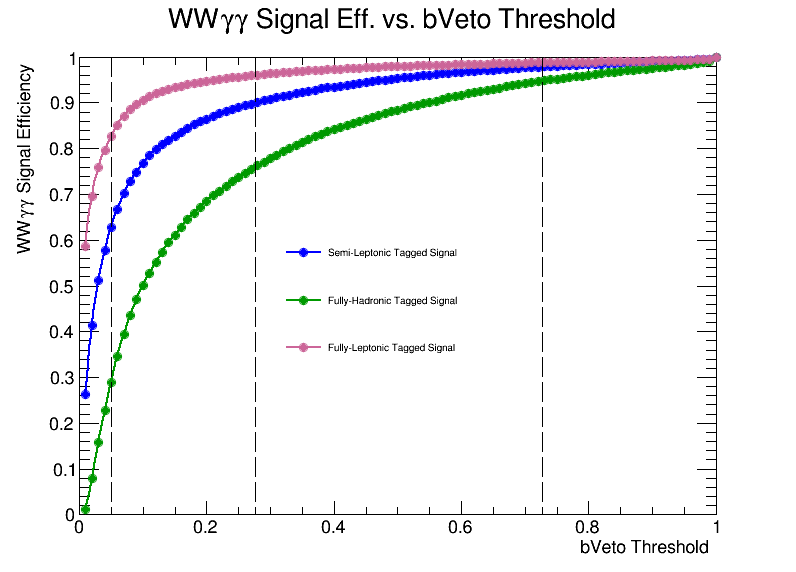
\includegraphics[width=0.45\textwidth]{Sections/HHWWgg/images/Objects/SigEffvsbVeto.png}}
    \qquad
    \subfloat[ttH]{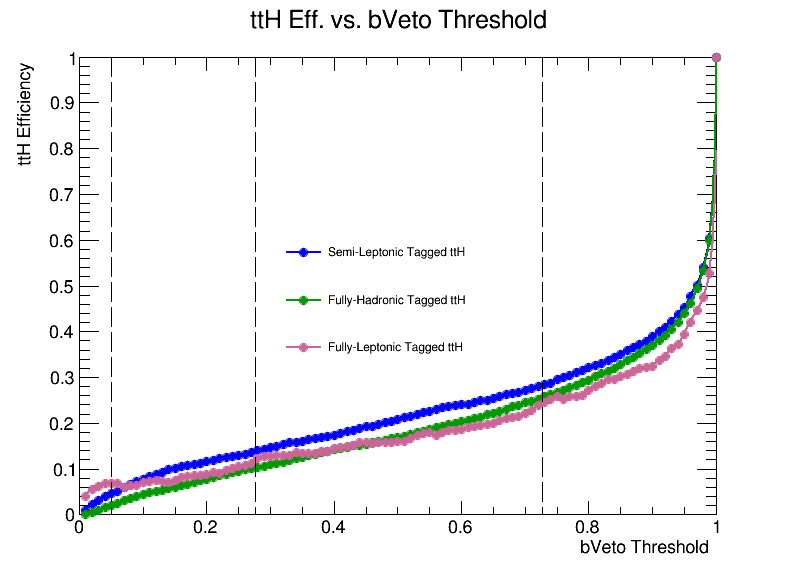
\includegraphics[width=0.45\textwidth]{Sections/HHWWgg/images/Objects/ttHvsbVeto.png}}
    \caption{2017 Signal and ttH background signal yields, relative to signal yield with no bVeto, vs. bVeto threshold}
    \label{fig:YieldVsBThresh}
\end{figure}

\begin{figure}[H]
    \centering
    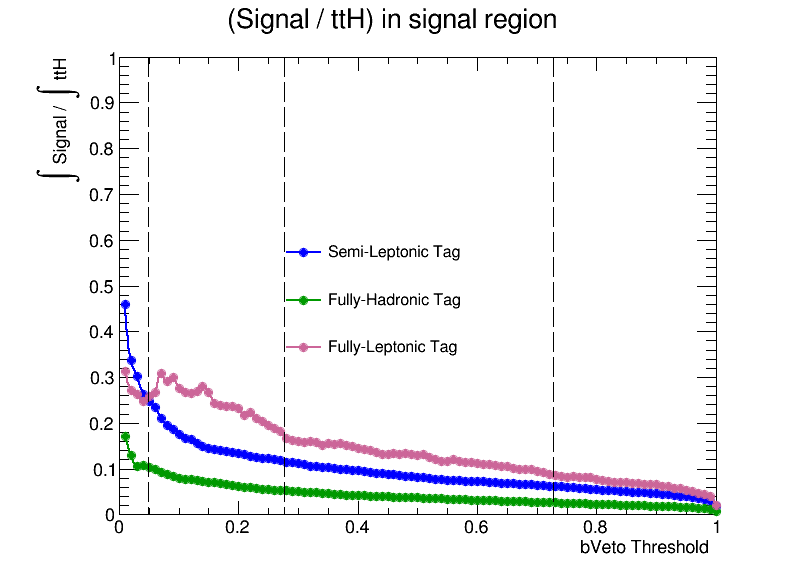
\includegraphics[width=0.75\textwidth]{Sections/HHWWgg/images/Objects/sigttHRatiovsbveto.png}
    \caption{Ratio of ttH signal region events over WW$\gamma\gamma$ signal events in signal region vs. bVeto threshold}
\label{fig:SigttHRatiovsbThresh}
\end{figure}

The signal efficiency curves look as expected for the three final states: The Fully-Leptonic final state is overall the most efficient because there are no quarks in its signal, Semi-Leptonic comes next
as it contains two quarks in its signal, and the Fully-Hadronic signal is the least efficient overall as it contains four quarks in its signal, and therefore is the most likely
to contain a jet with a higher b score due to high values of important b-tagging variables such as $p_{T}$. The ttH signal events as categorized by the three WW$\gamma\gamma$ categories have similar efficiencies among the three
categories, with about 75\% of events rejected from vetoing an event with at least one tightly b-tagged jet.

For the Semi-Leptonic and Fully-Hadronic final state categories, no b-veto is applied but rather is used as an input variable into DNN trainings. In order to properly reshape the MC b-tagging score distribution,
a btag-reshape scale factor is applied to these event weights for each jet passing event selections.

For the Fully-Leptonic final state category, the medium b-tagging score working point is applied as only about 5\% of signal is rejected, while about 85\% of ttH background is rejected.
Events falling into the fully-leptonic category are vetoed if they contain at least one jet with a b-tagging score greater than the medium working point.

The decision to apply a loose PU Jet ID to all jets with $p_{T}$ below 50 GeV comes from comparing the Fully-Hadronic final state category signal and data yields in the data sideband (defined as [100 $<$ $\mgg$ $<$ 115] or [135 $<$ $\mgg$ $<$ 180 GeV]) when applying
different PU Jet IDs. This category requires at least four jets, so applying different PU Jet ID requirements on all jets results in different yields, as shown in Figure \ref{fig:PUJetID},
with yields summarized in Table \ref{tab:PUJetIDYields}.

\begin{figure}[H]
    \setcounter{subfigure}{0}
    \centering
    \subfloat[Data Sidebands]{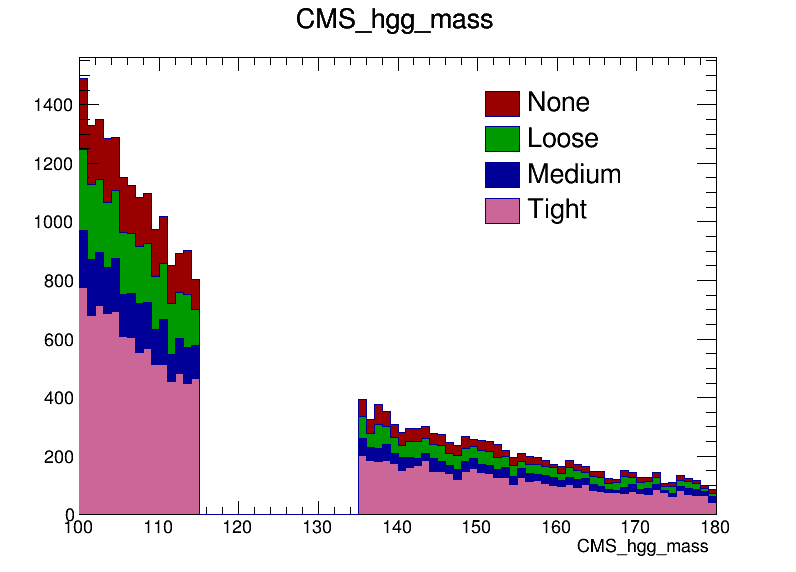
\includegraphics[width=0.45\textwidth]{Sections/HHWWgg/images/Objects/PUJet_ID_Sidebands.png}}
    \qquad
    \subfloat[Signal Region]{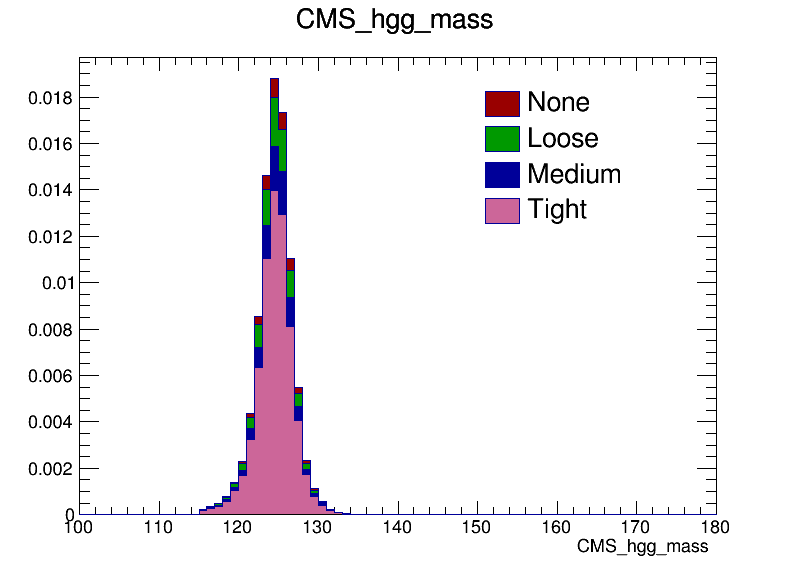
\includegraphics[width=0.45\textwidth]{Sections/HHWWgg/images/Objects/PUJet_ID_SR.png}}
    \caption{2017 Data (Signal) diphoton mass distributions in the sideband (signal) region for the Fully-Hadronic tagged category.}
    \label{fig:PUJetID}
\end{figure}

\begin{table}[!htbp]
    \begin{center}
            \begin{tabular}{|c|c|c|c|c||c|}
                    \hline
                    PUJet ID & Data Sidebands & Signal Region & Data Ratio to None & Signal Ratio to None & $\frac{S}{\sqrt{B}}$\\
                    \hline
                    None & 25940 & 0.09015 & 1 & 1 & 1 \\
                    \hline
                    Loose & 22119 & 0.08625 & 0.853 & 0.957 & 1.036 \\
                    \hline
                    Medium & 17418 & 0.07644 & 0.672 & 0.848 & 1.035\\
                    \hline
                    Tight & 14001 & 0.06707 & 0.540 & 0.744 & 1.012\\
                    \hline
            \end{tabular}
    \end{center}
    \caption{Number of data events in data sidebands and 2017 SM NLO Fully-Hadronic events in signal region, and relevant ratios. \label{tab:PUJetIDYields}}
\end{table}

If it is assumed that the relative change in dataside band events is roughly proportional to the relative change of data events in the signal region (defined as 115 $<$ $\mgg$ $<$ 135 GeV), an estimated signal region $\frac{S}{\sqrt{B}}$
can be computed and is found to be maximized in the case of applying a Loose PU Jet ID. A similar value is obtained when applying Medium PUJetID, but considering they are within
0.1\% of each other at the trade-off of a loss of about 10\% of signal, it is optimal to apply a loose PU Jet ID for the Fully-Hadronic final state. As the Semi-Leptonic and Fully-Leptonic
final state categories do not explicitly select on jet number, and the loose PU Jet ID has a high efficiency and should therefore not affect the Semi-Leptonic and Fully-Leptonic
final states noticeably, all jets are required to pass the Loose PU Jet ID.

\subsection{MET} \label{sec:MET}

The missing transverse momentum vector \ptvecmiss (sometimes referred to as ``MET") is defined as the projection onto the plane perpendicular to the beam axis of the negative vector sum of the momenta of all reconstructed PF objects in an event. Its magnitude is referred to as \ensuremath{\pt^\text{miss}}\xspace. This variable is of importance when identifying events which may contain a neutrino coming from a leptonic W decay, as neutrinos escape the CMS detector undetected.

In the Semi-Leptonic final state, MET is used as an input variable in the DNN training. In the Fully-Hadronic final state, MET is not used. In the Fully-Leptonic final state, a selection of 20 GeV is required for MET.
Corrections applied include an XY correction and MET filters, where the MET filters applied to Data and MC for all three years are shown in Table \ref{tab:METfilters} in order to remove events which are flagged as bad due to various reasons including large HCAL noise, dead ECAL channels. For Data there is one additional MET filter applied: {\tt Flag\_eeBadScFilter}, corresponding to events tagged as having poor ECAL endcap super clusters. 

\begin{table}[H]
    \begin{center}
        \begin{tabular}{c}
        MET Filters \\ \hline
        {\tt Flag\_goodVertices} \\
        {\tt Flag\_globalSuperTightHalo2016Filter} \\
        {\tt Flag\_HBHENoiseFilter} \\
        {\tt Flag\_HBHENoiseIsoFilter} \\
        {\tt Flag\_EcalDeadCellTriggerPrimitiveFilter} \\
        {\tt Flag\_BadPFMuonFilter} \\ 
        \end{tabular}
    \end{center}
    \caption{
        MET filters applied to Data and MC for all three years of data taking and detector conditions. 
    }
    \label{tab:METfilters}
\end{table}

\subsection{Preselection yields} \label{sec:Preselection_yields}

In this section, the yields and efficiencies of each 2017 signal and background MC process described in Section \ref{sec:samples} are shown before and after all object selections and final state preselections are applied in order to understand the major background processes to be targeted in each final state's subsequent selections. 

Preselections are defined as the common object and event selections described in the above subsections, in addition to the orthogonality selection applied for each final state: 
Events in the Semi-leptonic category are required to have exactly one lepton passing the common lepton selections, events in the Fully-hadronic category are required to have at least four jets and exactly 
zero leptons passing the common jet and lepton selections, and events in the Fully-leptonic category are required to have exactly 2 leptons passing the common lepton selections. 

The yields and process efficiencies before and after each final state's pre-selections are shown in Tables \ref{tab:Continuum_Background_Yield_Table}, \ref{tab:Single_Higgs_Yield_Table} and \ref{tab:HH_Yield_Table} below. Additionally,
the individual contribution of each MC sample with respect to the total MC yield for a given set of selections (Before preselection, Semi-leptonic preselections, Fully-hadronic preselections or Fully-Leptonic preselections)
are shown in Tables \ref{tab:Continuum_Background_Contribution_Table} and \ref{tab:Single_Higgs_Contribution_Table}. Note that processes with an absolute number of simulated events less than 1000 (less than 100 in the fully-leptonic final category) are given a null value or only an efficiency is reported, as their low number of events implies that their corresponding processes would have a poor simulated description and potentially a large statistical uncertainty. 

\begin{figure}[H]
        \resizebox{1\textwidth}{!}{%
                \begin{tabular}{c|c|c|c|c}
                        MC Sample & Before preselection & SL (efficiency) & FH (efficiency) & FL (efficiency) \\ \hline
                         %DiPhotonJetsBox\_M40\_80 & 1138.8964 & - (-\%) & - (-\%) & - (-\%) \\
                         $\gamma\gamma+$jets & 302977.6194 & 542.4641 (0.179\%) & 6246.9949 (2.062\%) & 2.7749 (0.001\%) \\
                        %  DYJetsToLL\_M-50 & 7525.2616 & - (-\%) & - (-\%) & - (-\%) \\
                         THQ\_ctcvcp & 3.4592 & 0.5789 (16.735\%) & 1.0579 (30.582\%) & 0.0012 (0.034\%) \\
                         TTGG\_0Jets & 44.0507 & 10.9847 (24.936\%) & 25.6024 (58.12\%) & 0.1487 (0.338\%) \\
                         TTGJets\_TuneCP5 & 765.4892 & 154.6684 (20.205\%) & 402.1377 (52.533\%) & ($<$0.2\%) \\
                        %  TTToHadronic & 903.4816 & - (-\%) & - (-\%) & - (-\%) \\
                         ttWJets & 5.0469 & ($\approx$21\%) & 2.8337 (56.147\%) & ($<$0.1\%) \\
                        %  W3JetsToLNu & 1041.188 & - (-\%) & - (-\%) & - (-\%) \\
                        %  W4JetsToLNu & 985.8018 & - (-\%) & - (-\%) & - (-\%) \\
                        %  WGGJets & 534.8559 & - (-\%) & - (-\%) & - (-\%) \\
                        %  WGJJToLNu\_EWK\_QCD & 367.5752 & - (-\%) & - (-\%) & - (-\%) \\
                        %  WGJJToLNuGJJ\_EWK & 65.3279 & - (-\%) & - (-\%) & - (-\%) \\
                        %  WWTo1L1Nu2Q & 337.0574 & - (-\%) & - (-\%) & - (-\%) \\
                        %  WW\_TuneCP5 & 189.1288 & - (-\%) & - (-\%) & - (-\%) \\
                         GJet & 830909.3171 & 1061.0649 (0.002\%) & 2466.3582 (0.002\%) & ($<$0.001\%) \\
                         QCD & 1653618.4935 & ($<$0.001\%) & ($<$0.001\%) & ($<$0.001\%) \\
                         TTJets & 23.5628 & 3.3477 (81.397\%) & 18.8106 (55.121\%) & ($<$2\%) \\
                         W1Jet & 5838.2419 & 245.2825 (0.329\%) & ($<$0.5\%) & ($<$0.5\%) \\
                         W2Jets & 5589.4864 & 352.6322 (0.343\%) & 204.2186 (0.232\%) & ($<$0.5\%) \\ \hline
                         Total & 2812863.3417 & 2371.0234 (0.0008\%) & 9368.014 (0.0033\%) & 2.9248 (0.0\%) \\ \hline
                \end{tabular}}
        \captionof{table}{2017 Continuum Background MC before and after preselections for each final state, and process efficiency. Note that for processes with less than 1000 unweighted MC events after a selection (100 for the fully-leptonic preselections), a null value or only efficiency is shown.}
        \label{tab:Continuum_Background_Yield_Table}
\end{figure}

\newpage 

\begin{figure}[H]
        \resizebox{1\textwidth}{!}{%
                \begin{tabular}{c|c|c|c|c}
                        MC Sample & Before preselection & SL & FH & FL \\ \hline
                         %DiPhotonJetsBox\_M40\_80 & 0.0405\% & -\% & -\% & -\% \\
                         $\gamma\gamma+$jets & 10.7711\% & 22.8789\% & 66.6843\% & 94.8755\% \\
                        %  DYJetsToLL\_M-50 & 0.2675\% & -\% & -\% & -\% \\
                         THQ\_ctcvcp & 0.0001\% & 0.0244\% & 0.0113\% & 0.0397\% \\
                         TTGG\_0Jets & 0.0016\% & 0.4633\% & 0.2733\% & 5.0849\% \\
                         TTGJets\_TuneCP5 & 0.0272\% & 6.5233\% & 4.2927\% & -\% \\
                        %  TTToHadronic & 0.0321\% & -\% & -\% & -\% \\
                         ttWJets & 0.0002\% & -\% & 0.0302\% & -\% \\
                        %  W3JetsToLNu & 0.037\% & -\% & -\% & -\% \\
                        %  W4JetsToLNu & 0.035\% & -\% & -\% & -\% \\
                        %  WGGJets & 0.019\% & -\% & -\% & -\% \\
                        %  WGJJToLNu\_EWK\_QCD & 0.0131\% & -\% & -\% & -\% \\
                        %  WGJJToLNuGJJ\_EWK & 0.0023\% & -\% & -\% & -\% \\
                        %  WWTo1L1Nu2Q & 0.012\% & -\% & -\% & -\% \\
                        %  WW\_TuneCP5 & 0.0067\% & -\% & -\% & -\% \\
                         GJet & 29.5396\% & 44.7513\% & 26.3274\% & -\% \\
                         QCD & 58.7877\% & -\% & -\% & -\% \\
                         TTJets & 0.0008\% & 0.1412\% & 0.2008\% & -\% \\
                         W1Jet & 0.2076\% & 10.345\% & -\% & -\% \\
                         W2Jets & 0.1987\% & 14.8726\% & 2.18\% & -\% \\ \hline
                         Total & 100\% & 100\% & 100\% & 100\% \\ \hline
                \end{tabular}}
        \captionof{table}{Contribution w.r.t total 2017 Continuum Background MC for various phase spaces: Before and after preselections for each final state. Note that for processes with less than 1000 unweighted MC events after a selection (100 for the fully-leptonic preselections), a null value is shown.}
        \label{tab:Continuum_Background_Contribution_Table}
\end{figure}

\newpage 

\begin{figure}[H]
        \resizebox{1\textwidth}{!}{%
                \begin{tabular}{c|c|c|c|c}
                        MC Sample & Before preselection & SL (efficiency) & FH (efficiency) & FL (efficiency) \\ \hline
                         GluGluHToGG & 2226.7151 & 2.5556 (0.115\%) & 18.3933 (0.826\%) & - (-\%) \\
                         ttHJetToGG & 23.8639 & 5.9022 (24.733\%) & 14.4288 (60.463\%) & 0.0545 (0.228\%) \\
                         VBFHToGG & 158.1456 & 0.3712 (0.235\%) & 1.0675 (0.675\%) & - (-\%) \\
                         VHToGG & 85.5536 & 10.0542 (11.752\%) & 4.4384 (5.188\%) & 0.0832 (0.097\%) \\ \hline
                         Total MC & 2494.2782 & 18.8832 (0.0076\%) & 38.328 (0.0154\%) & 0.1377 (0.0001\%) \\ \hline
                \end{tabular}}
        \captionof{table}{2017 Single Higgs MC before and after preselections for each final state, and process efficiency. Note that for processes with less than 100 unweighted MC events after a selection, a null value is shown.}
        \label{tab:Single_Higgs_Yield_Table}
\end{figure}

\begin{figure}[H]
        \resizebox{1\textwidth}{!}{%
                \begin{tabular}{c|c|c|c|c}
                        MC Sample & Before preselection & SL & FH & FL \\ \hline
                         GluGluHToGG & 89.3\% & 13.5\% & 48\% & -\% \\
                         ttHJetToGG & 0.96\% & 31.3\% & 37.6\% & 39.6\% \\
                         VBFHToGG & 6.34\% & 2.0\% & 2.8\% & -\% \\
                         VHToGG & 3.43\% & 53\% & 11.6\% & 60.4\% \\ \hline
                         Total & 100\% & 100\% & 100\% & 100\% \\ \hline
                \end{tabular}}
        \captionof{table}{Contribution w.r.t total 2017 Single Higgs MC for various phase spaces: Before and after preselections for each final state. Note that for processes with less than 1000 unweighted MC events after a selection (100 for the fully-leptonic preselections), a null value is shown.}
        \label{tab:Single_Higgs_Contribution_Table}
\end{figure}

\begin{figure}[H]
        \resizebox{1\textwidth}{!}{%
            \begin{tabular}{c|c|c|c|c}
                    MC Sample & Before preselection & SL (efficiency) & FH (efficiency) & FL (efficiency) \\ \hline
                     Semi-leptonic HH$\rightarrow WW\gamma\gamma$ & 0.3042 & 0.1044 (34.306\%) & - (-\%) & - (-\%) \\
                     Fully-hadronic HH$\rightarrow WW\gamma\gamma$ & 0.3012 & - (-\%) & 0.0966 (32.07\%) & - (-\%) \\
                     Fully-leptonic HH$\rightarrow WW\gamma\gamma$ & 0.0741 & - (-\%) & - (-\%) & 0.0098 (13.214\%) \\ \hline 
            \end{tabular}}
    \captionof{table}{2017 HH MC before and after preselections for each final state, and process efficiency. Note that for processes with less than 100 unweighted MC events after a selection, a null value is shown.} 
    \label{tab:HH_Yield_Table}
\end{figure}


The tables show that among the continuum background MC processes, the fully-leptonic final state has a very low absolute number of simulation events after pre-selections and requiring exactly two leptons passing the common lepton selections. This was a core reason for the decision to perform a cut-based analysis for this final state, as there are not nearly enough MC events in order to perform a reasonable MVA based analysis. In the fully-hadronic final state, where a large QCD multi-jet background is expected, there is a low absolute number of simulation events from QCD MC, prompting the use of a data-driven estimate of QCD. For all three final states, the non-resonant diphoton $+$ jets process acts as a major background. 

The single higgs resonant background tables indicate that, as expected, different single higgs processes have larger background contaminations among the different WW$\gamma\gamma$ final states due to their different process topologies. However, for all final states the ttH process has a relatively high efficiency due to the presence of two top quarks which decay into bbWW in the majority of cases. 

Finally, it is seen in the HH selection table that the semi-leptonic and fully-hadronic signal processes have similar signal efficiencies and yields after pre-selections. This may be due to their relatively high branching ratios compared to the FL final state. 
\clearpage
\section{Selections and Categorization} \label{fig:HHWWgg_SelectionsAndCat}

After implementing the object reconstruction defined in Section \ref{sec:Objects}, each final state performs additional selection and categorization techniques specific to its final state topology.

For all three final states, the distribution of signal events has a peak in the diphoton invariant mass, \mgg, distribution around the mass of the Higgs boson (125 GeV). The analysis strategy is therefore based on defining regions of phase space sensitive to the diphoton mass peak around 125 GeV containing as many HH events as possible, while minimizing the yields of the continuum background and resonant single Higgs backgrounds. However, because each WW$\gamma\gamma$ final state has its own signal topology, dominant background processes and absolute number of simulation events, each final state employs a separate strategy for further selections and categorization techniques after the pre-selections defined in Section \ref{sec:Objects}.

This section is organized as follows: In Section \ref{sec:SL_Selections}, the semi-leptonic final state selections and categorization, including the use of multiple DNNs, will be described. In Section \ref{subsec:FullyHadronicEventSelection}, the fully-hadronic final state selections and categorization, which also make use of DNN methods will be described. Finally, in Section \ref{sec:FullyLeptonicEventSelections} the fully-leptonic final state selections will be described. 

% Semi-Leptonic
\subsection{Semi-Leptonic} \label{sec:SL_Selections}

Events fall into the Semi-Leptonic analysis category if they contain at least one pre-selected diphoton as described in Section \ref{sec:photons}, and contain 
exactly one lepton passing the common lepton selections described in Section \ref{sec:LeptonSelections}. The Semi-Leptonic channel is expected to be the most 
sensitive of the three WW$\gamma\gamma$ channels due to the combination of a relatively large $W\rightarrow qq$ branching ratio of $\approx$ 67\%, and the presence of a clean, highly energetic 
lepton from the $W\rightarrow\ell\nu$ decay leg. 

The four NLO generated Semi-Leptonic signal events corresponding to the points $\kappa_{\lambda}$ = [0, 1 (SM), 2.45, 5], and a set of samples coming from a reweighting of these four samples to the points $3D3$ ($\kappa_{\lambda}$ = 0, $\kappa_{t}$ = 1.0, $c_{ttHH}$ = 1.0), $c_{ttHH}$ = 3, and $c_{ttHH}$ = 0.35 are categorized with a multi-class DNN, where $c_{ttHH}$ represents the coupling strength of two top quarks to two Higgs bosons. These corresponding simulation templates are used to model the Semi-Leptonic HH final state for the SM hypothesis, and to perform scans of the $\kappa_{\lambda}$ and $c_{2}$ EFT parameters. 

The four generated NLO samples are reweighted to the 20 EFT benchmarks, and categorized using a parametric DNN which includes the EFT benchmark scenario number as a training variable. The resulting categorized simulation templates are used to model the semi-leptonic HH final state for these 20 scenarios. 

\subsubsection{Standard Model: Multiclass Deep Neural Network}

For a general description of Deep Neural Networks, see Appendix \ref{sec:DNN}. 

In the Semi-Leptonic category, in order to separate the di-Higgs signal from the expected single Higgs boson and continuum backgrounds, a multiclass deep neural network is trained to identify these three types of processes 
separately, in order to identify regions of phase space with a maximal number of HH events, but a minimal number of single H and continuum background events. Because the single higgs and continuum background 
processes are markedly different due to the expectation of a resonant H signal vs. a falling continuum background, as shown in Figure \ref{fig:Signatures}, it is more logical to define these two processes separately in a DNN training rather 
than defining them as the same type of background. 

% The multiclass DNN is trained using 2017 signal and background samples, and is evaluated on 2016, 2017 and 2018 signal samples for analytic fitting, and on Run 2 CMS data 
% to be used for categorization and data-driven background modeling. The 12 generated LO EFT benchmark samples, as well as the LO SM benchmark, are reweighted to the SM HH process at NLO and are combined and considered together as 
% signal in the training.

% The network is trained on a labelled dataset where the 2017 HH process is defined as signal, and single higgs and non-Higgs datasets which are defined as separate classes. The single higgs processes
% trained on are the associated VH and ttH production modes of $H\rightarrow\gamma\gamma$.

The samples used for training and labeled as signal are the 12 LO benchmark samples, as well as the LO SM benchmark, where all thirteen simulation samples include 2017 detector conditions for reconstruction. When training on these 
samples, the reweighting procedure described in Section \ref{sec:EFT_Description}
is applied to reweight these LO EFT benchmark and SM sample to the SM process at NLO, in order to train the network to identify the SM at NLO HH signal. 
In deriving these weights, NLO samples are reweighted following \cite{Buchalla:2018yce}, and LO samples are reweighted 
following an analytic parameterization as a function of $\sigma_{HH}$ and $|\cos{\theta^*}|$ which extends beyond $m_{HH} = 1050$ GeV, and the ratio of the two is taken 
and normalized by Equation \ref{eq:LONLONorm}, yielding an event by event weight. These event weights scale the per-event training loss in order to 
assign more training importance to events which must be weighted up in order to match SM NLO. 

The ratio of a few of the DNN's input variable distributions between the sum of reweighted 13 LO benchmarks (12 + SM at LO), and the 2017 SM at NLO signal are shown in Figures \ref{fig:LO_NLO_Reweight_CrPlts-1} and \ref{fig:LO_NLO_Reweight_CrPlts-2}, and the rest are shown in Appendix \ref{sec:DNN-Input-Variables-LO_NLO_Weight_Validation}.

\begin{figure}[h!]
    \setcounter{subfigure}{0}
    \centering
    \subfloat[Scaled Leading Photon \pt]{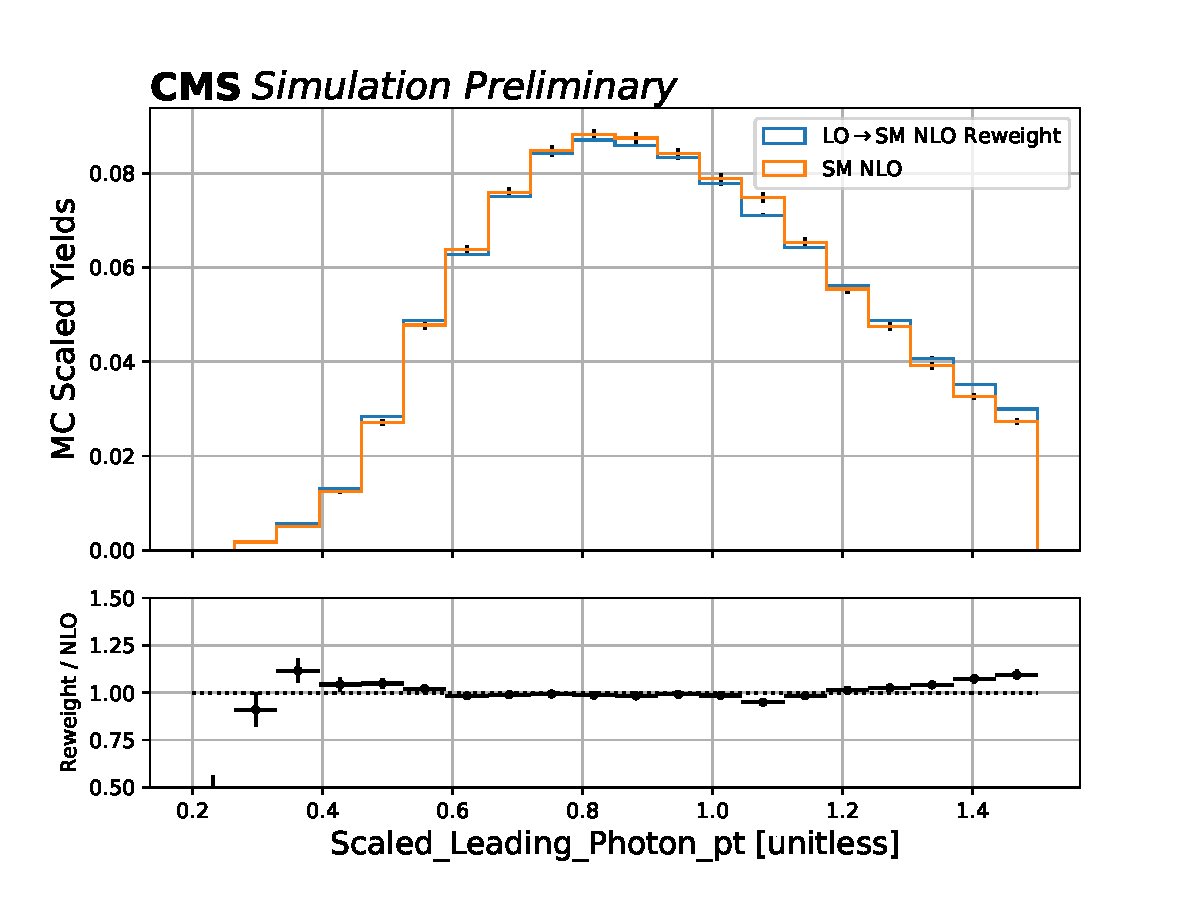
\includegraphics[width=0.475\textwidth]{Sections/HHWWgg/images/DNN/LO_NLO_Reweight_Distributions/Scaled_Leading_Photon_pt.pdf}}
    \subfloat[Scaled subleading photon \pt]{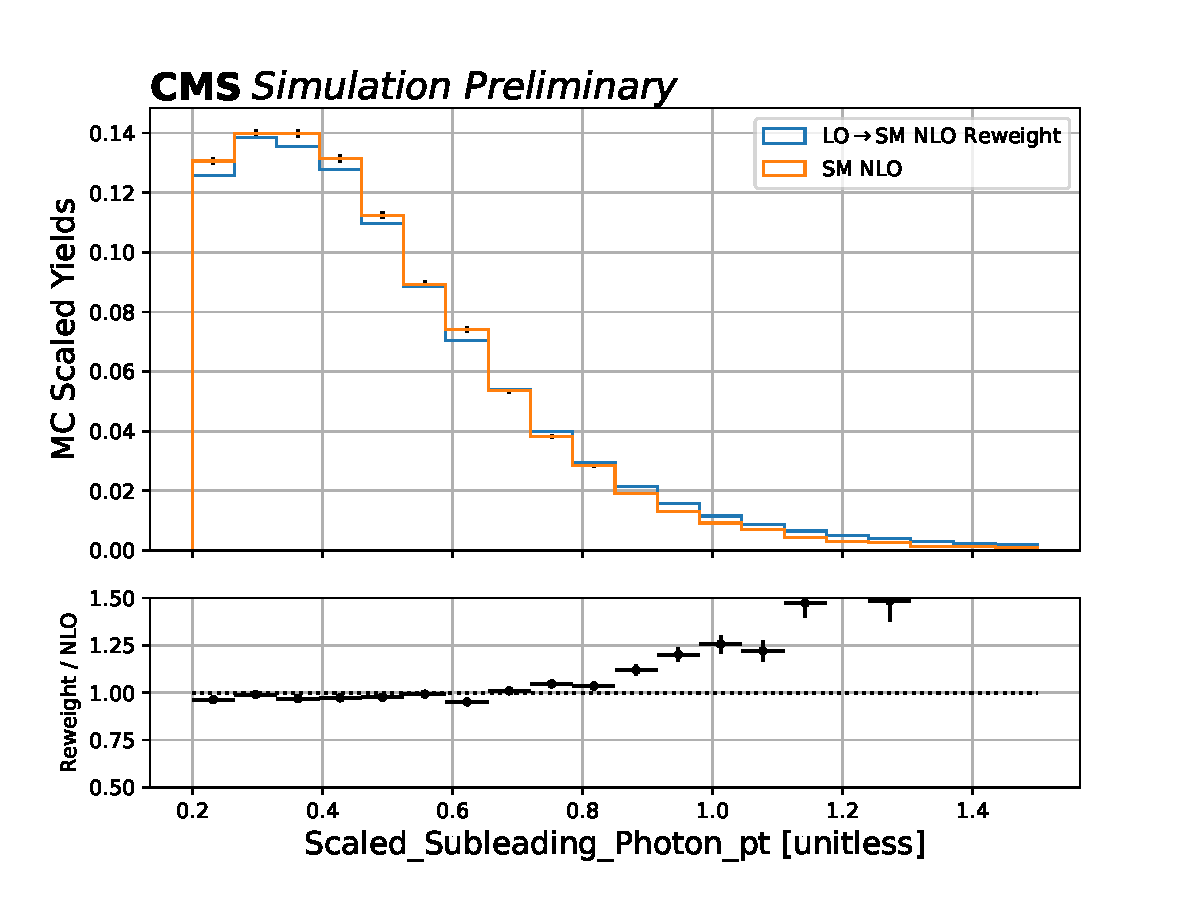
\includegraphics[width=0.475\textwidth]{Sections/HHWWgg/images/DNN/LO_NLO_Reweight_Distributions/Scaled_Subleading_Photon_pt.pdf}}
    \caption{Scaled leading and subleading photon \pt. \label{fig:LO_NLO_Reweight_CrPlts-1}}
\end{figure}
    
\begin{figure}[h!]
    \setcounter{subfigure}{0}
    \centering
    \subfloat[Lepton $p_{T}$]{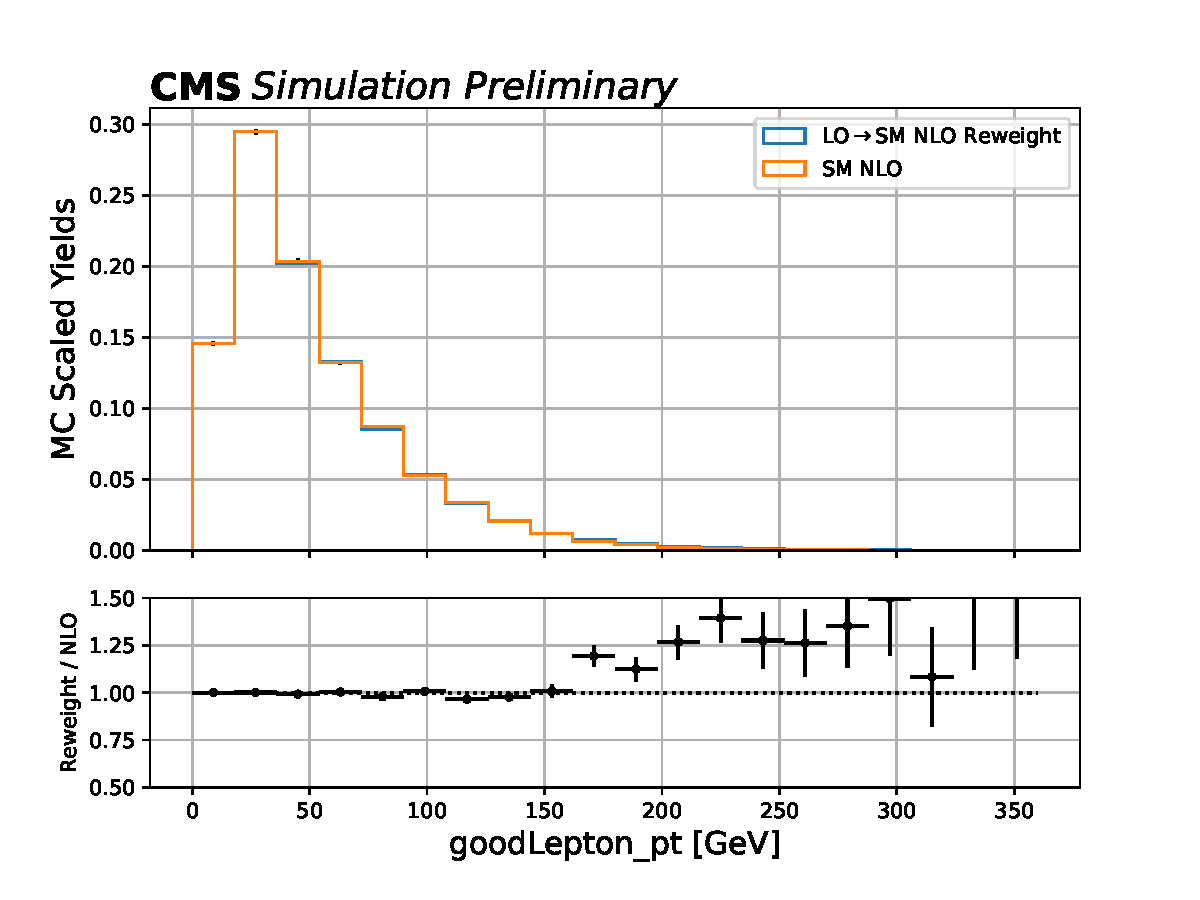
\includegraphics[width=0.475\textwidth]{Sections/HHWWgg/images/DNN/LO_NLO_Reweight_Distributions/goodLepton_pt.pdf}}
    \subfloat[MET]{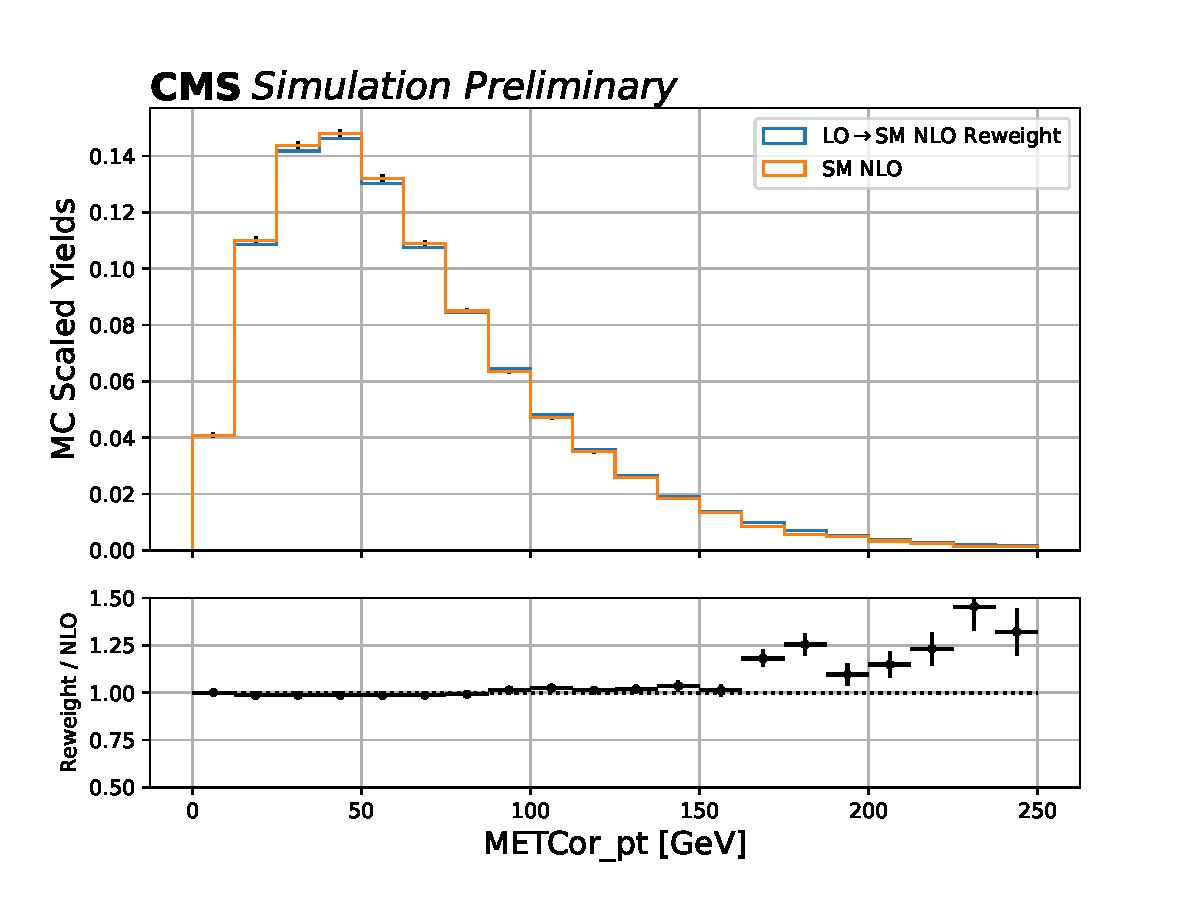
\includegraphics[width=0.475\textwidth]{Sections/HHWWgg/images/DNN/LO_NLO_Reweight_Distributions/METCor_pt.pdf}}
    \caption{Lepton \pt and MET\label{fig:LO_NLO_Reweight_CrPlts-2}}
\end{figure}

There is good agreement overall, indicating that training on these events and including the LO to NLO event reweighting in the training via loss scaling trains a network geared towards identifying the SM and NLO signal.

The samples used for training and labeled as single Higgs processes are the associated production of a Higgs boson with a vector boson (VH), and with a top quark pair (ttH), where the Higgs decays to $\gamma\gamma$ in both cases. 

The samples used for training and labeled as continuum background were chosen based on the background MC processes which have at least 1000 absolute events after the semi-leptonic pre-selections, such that there is no large statistical uncertainty on these process descriptions. 

Events used to train the network are required to contain at least one diphoton candidate passing the common diphoton selections described in Section \ref{sec:photons},
and contain exactly one lepton passing the common lepton selections in Section \ref{sec:LeptonSelections}.

Due to the class imbalance in the datasets, events are re-weighted with a per-class ``class weight", such that after applying this weight, the effective number 
of events in both classes is the same. In deriving each class weight, a class's weighted MC yield is scaled to the unweighted HH yield of 866,833. This ensures that the network focuses on categorizing all three classes with equal importance. The unweighted and weighted yields, 
and class weights of all training events which have only diphoton pre-selections applied and the requirement of exactly one lepton passing the common lepton selections, 
are shown in Table \ref{tab:yieldsAndClassWeights}. Note that 
in Table \ref{tab:yieldsAndClassWeights}, HH events are not normalized to cross section and branching ratio,
as this is not necessary because all weighted yields are reweighted to a common target, and therefore what is relevant are the relative yields. 

\begin{figure}[H]
        \resizebox{1\textwidth}{!}{%
          \begin{tabular}{c|c|c|c|c} 
                  Class & Unweighted Yield & Weighted Yield & Class Weight & Class Weight * Weighted Yield \\ \hline
                   HH & 866833 & 2.232871 & 388214 & 866833 \\
                   H & 78108 & 1.057757 & 819501 & 866833 \\
                   Continuum Background & 61408 & 16104 & 53.8278 & 866833 \\ \hline 
          \end{tabular}}
        \captionof{table}{Unweighted and weighted yields, and class weights applied during Semi-Leptonic DNN training, without data sideband scale. Weighted class yields are reweighted by class weights to the unweighted HH yield. \label{tab:yieldsAndClassWeights}}
        
\end{figure}

The features used as input to the semi-leptonic channel DNN can be found in Table \ref{tab:SLinputvars}. 

\begin{table}[H]
\caption{Input features used to train semi-leptonic channel DNN.}
\resizebox{\textwidth}{!}{
\begin{tabular}{| l | l |}
\hline
Feature & Description \\
\hline
Leading Photon p$_T$ / \mgg& Transverse momentum of the photon with the highest transverse momentum out of the selected photons, scaled to diphoton mass. \\
Leading Photon $\eta$ & Pseudorapidity of the photon with the highest transverse momentum out of the selected photons \\
Leading Photon $\phi$ & Direction in the transverse plane of the photon with the highest transverse momentum out of the selected photons \\
Leading Photon E / \mgg& Energy of the photon with the highest transverse momentum out of the selected photons, scaled to diphoton mass. \\
Leading Photon MVA & Photon MVA score of the photon with the highest transverse momentum out of the selected photons \\
Subleading Photon p$_T$  / \mgg& Transverse momentum of the photon with the second highest transverse momentum out of the selected photons, scaled to diphoton mass. \\
Subleading Photon $\eta$ & Pseudorapidity of the photon with the second highest transverse momentum out of the selected photons \\
Subleading Photon $\phi$ & Direction in the transverse plane of the photon with the second highest transverse momentum out of the selected photons \\
Subleading Photon E / \mgg & Energy of the photon with the second highest transverse momentum out of the selected photons, scaled to diphoton mass. \\
Subleading Photon MVA & Photon MVA score of the photon with the second highest transverse momentum out of the selected photons \\
Jet Multiplicity & Number of selected jets in the event (flavour inclusive) \\
Leading Jet p$_T$ & Transverse momentum of the jet with the highest transverse momentum out of the selected jets \\
Leading Jet $\eta$ & Pseudorapidity of the jet with the highest transverse momentum out of the selected jets \\
Leading Jet $\phi$ & Direction in the transverse plane of the jet with the highest transverse momentum out of the selected jets \\
Leading Jet E & Energy of the jet with the highest transverse momentum out of the selected jets \\
Leading Jet DeepJet Score & DeepJet b-tag discriminator score of the jet with the highest transverse momentum out of the selected jets \\
Subleading Jet p$_T$ & Transverse momentum of the jet with the second highest transverse momentum out of the selected jets \\
Subleading Jet $\eta$ & Pseudorapidity of the jet with the second highest transverse momentum out of the selected jets \\
Subleading Jet $\phi$ & Direction in the transverse plane of the jet with the second highest transverse momentum out of the selected jets \\
Subleading Jet E & Energy of the jet with the second highest transverse momentum out of the selected jets \\
Subleading Jet DeepJet Score & DeepJet b-tag discriminator score of the jet with the second highest transverse momentum out of the selected jets \\
Lepton p$_{T}$ & Transverse momentum of the selected lepton \\ 
Lepton $\eta$ & Pseudorapidity of the selected lepton \\ 
Lepton $\phi$ & Direction in the transverse plane of the selected lepton \\ 
Lepton E & Energy of the selected lepton \\ 
MET & The missing transverse energy \\ 
$M_{T}$(l, MET) & The transverse mass of the selected lepton and MET \\
$m_{j_{0},j_{1}}$ & The invariant mass of the leading and subleading jets \\ 
\hline
\end{tabular}
}
\label{tab:SLinputvars}
\end{table}

To determine the level of optimization of the network towards CMS data by training on MC, the data-MC ratio is checked for input features in the data sideband region after the semi-leptonic preselections are applied. Disagreements are seen between data and MC in the data sideband (100 $<$ $\mgg$ $<$ 115 or 135 $<$ $\mgg$ $<$ 180 GeV), as shown for various input features shown 
in Figures \ref{fig:Kin_Reweight_0_withoutKinWeights}, 
\ref{fig:Kin_Reweight_1_withoutKinWeights}, \ref{fig:Kin_Reweight_2_withoutKinWeights}, \ref{fig:Kin_Reweight_3_withoutKinWeights}, \ref{fig:Kin_Reweight_4_withoutKinWeights}, and
\ref{fig:Kin_Reweight_5_withoutKinWeights}. In
order to improve data/MC agreement so that the input features of the DNN are closer to a representation of the data in order to train a DNN more optimally, a 6-dimensional kinematic reweighting is performed. 

A per-event weight, called a kinematic weight, is computed as the ratio between data and background MC from the $\mgg$ sideband region (Note that data events in the signal region, 115 $<$ $\mgg$ $<$ 135 GeV, are not used at all when deriving
the kinematic weights). The variables Leading Jet \pt, Subleading Jet \pt, Lepton \pt, 
Leading Photon \pt over \mgg, Subleading Photon \pt over \mgg, and MET are used to calculate this per-event weight, as they correspond to quantities related to the semi-leptonic WW$\gamma\gamma$ final state particles. During the derivation of the weights, 5 bins are used for each variable. The range of each 
bin is selected in an automatic way such that there are the same number of data events in each bin. When the number of data events in a bin is lower than 20, the kinematic weight is set to 1. Otherwise,
the weight is set equal to the ratio (data entries)/(MC entries). 
After the kinematic weights are derived, a fiducial selection is made removing all events 
which have $|w_{MC}*w_{k}| > 10$, where $w_{MC}$ is the nominal MC weight computed from cross section, luminosity, PU weight, scale factors and GEN weights, and $w_{k}$ represents the per event kinematic weight. 
This fiducial selection removes events with very large weights which heavily impact the DNN training in a non-desirable way. 

The data/MC after applying the per-event kinematic weights, in the data sideband (100 $<$ $\mgg$ $<$ 115 or 135 $<$ $\mgg$ $<$ 180 GeV) and before any evaluation of the DNN, are shown in Figures \ref{fig:Kin_Reweight_0_withKinWeights}, 
\ref{fig:Kin_Reweight_1_withKinWeights}, \ref{fig:Kin_Reweight_2_withKinWeights}, \ref{fig:Kin_Reweight_3_withKinWeights}, \ref{fig:Kin_Reweight_4_withKinWeights}, \ref{fig:Kin_Reweight_5_withKinWeights}. It can be 
seen that the application of the kinematic weights improves the data/MC agreement, especially in very high yield bins. It can also be seen that after applying the kinematic reweighting there is no 
introduction of extremely large statistical uncertainties or fluctuations, indicating that there is a sufficient amount of data and MC events in deriving the kinematic weights. 

\newpage 

\begin{figure}[h!]
    \setcounter{subfigure}{0}
    \centering
    \subfloat[Before kinematic reweighting applied]{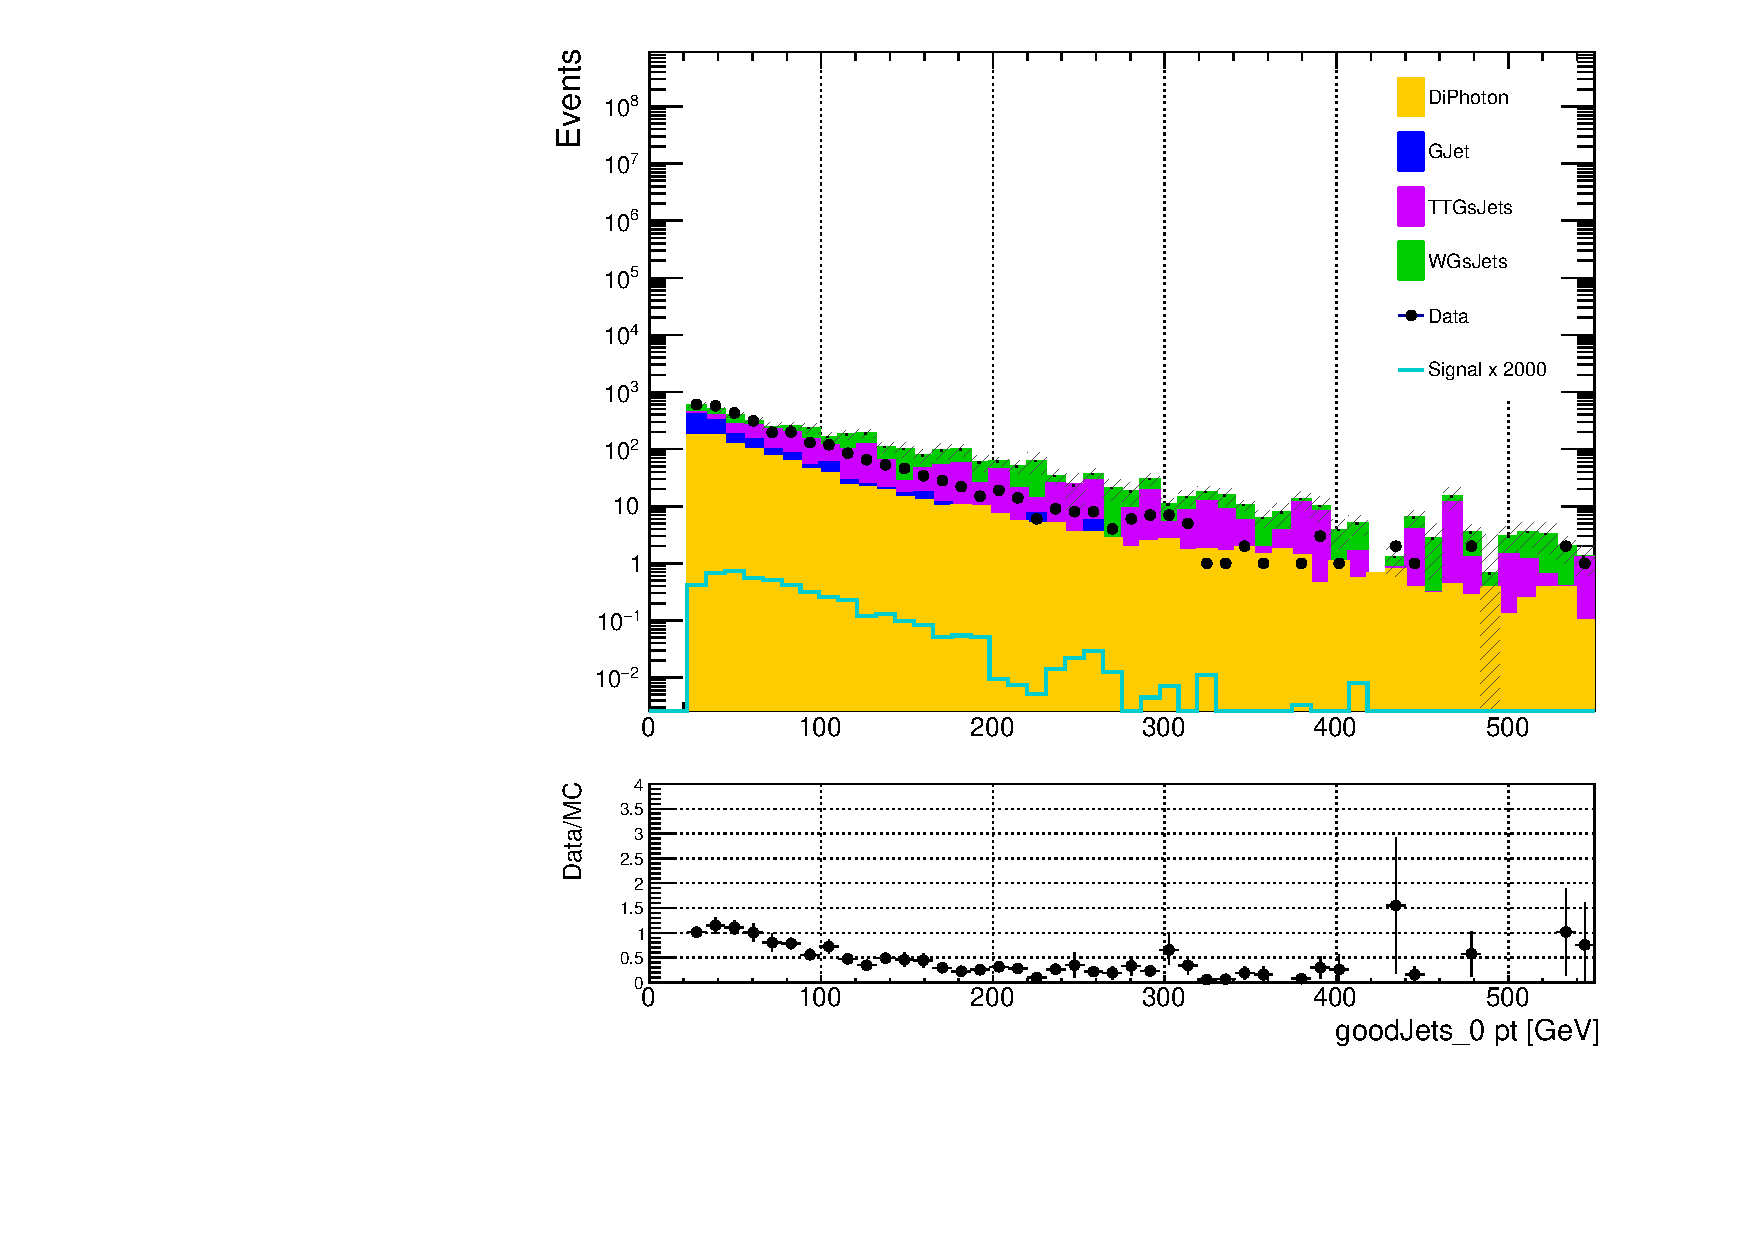
\includegraphics[width=0.45\textwidth]{Sections/HHWWgg/images/Semileptonic_Kinematic_Reweighting/Data_MC_WithoutKinWeights/goodJets_0_pt_log.pdf}\label{fig:Kin_Reweight_0_withoutKinWeights}} 
    \qquad     
    \subfloat[After kinematic reweighting applied]{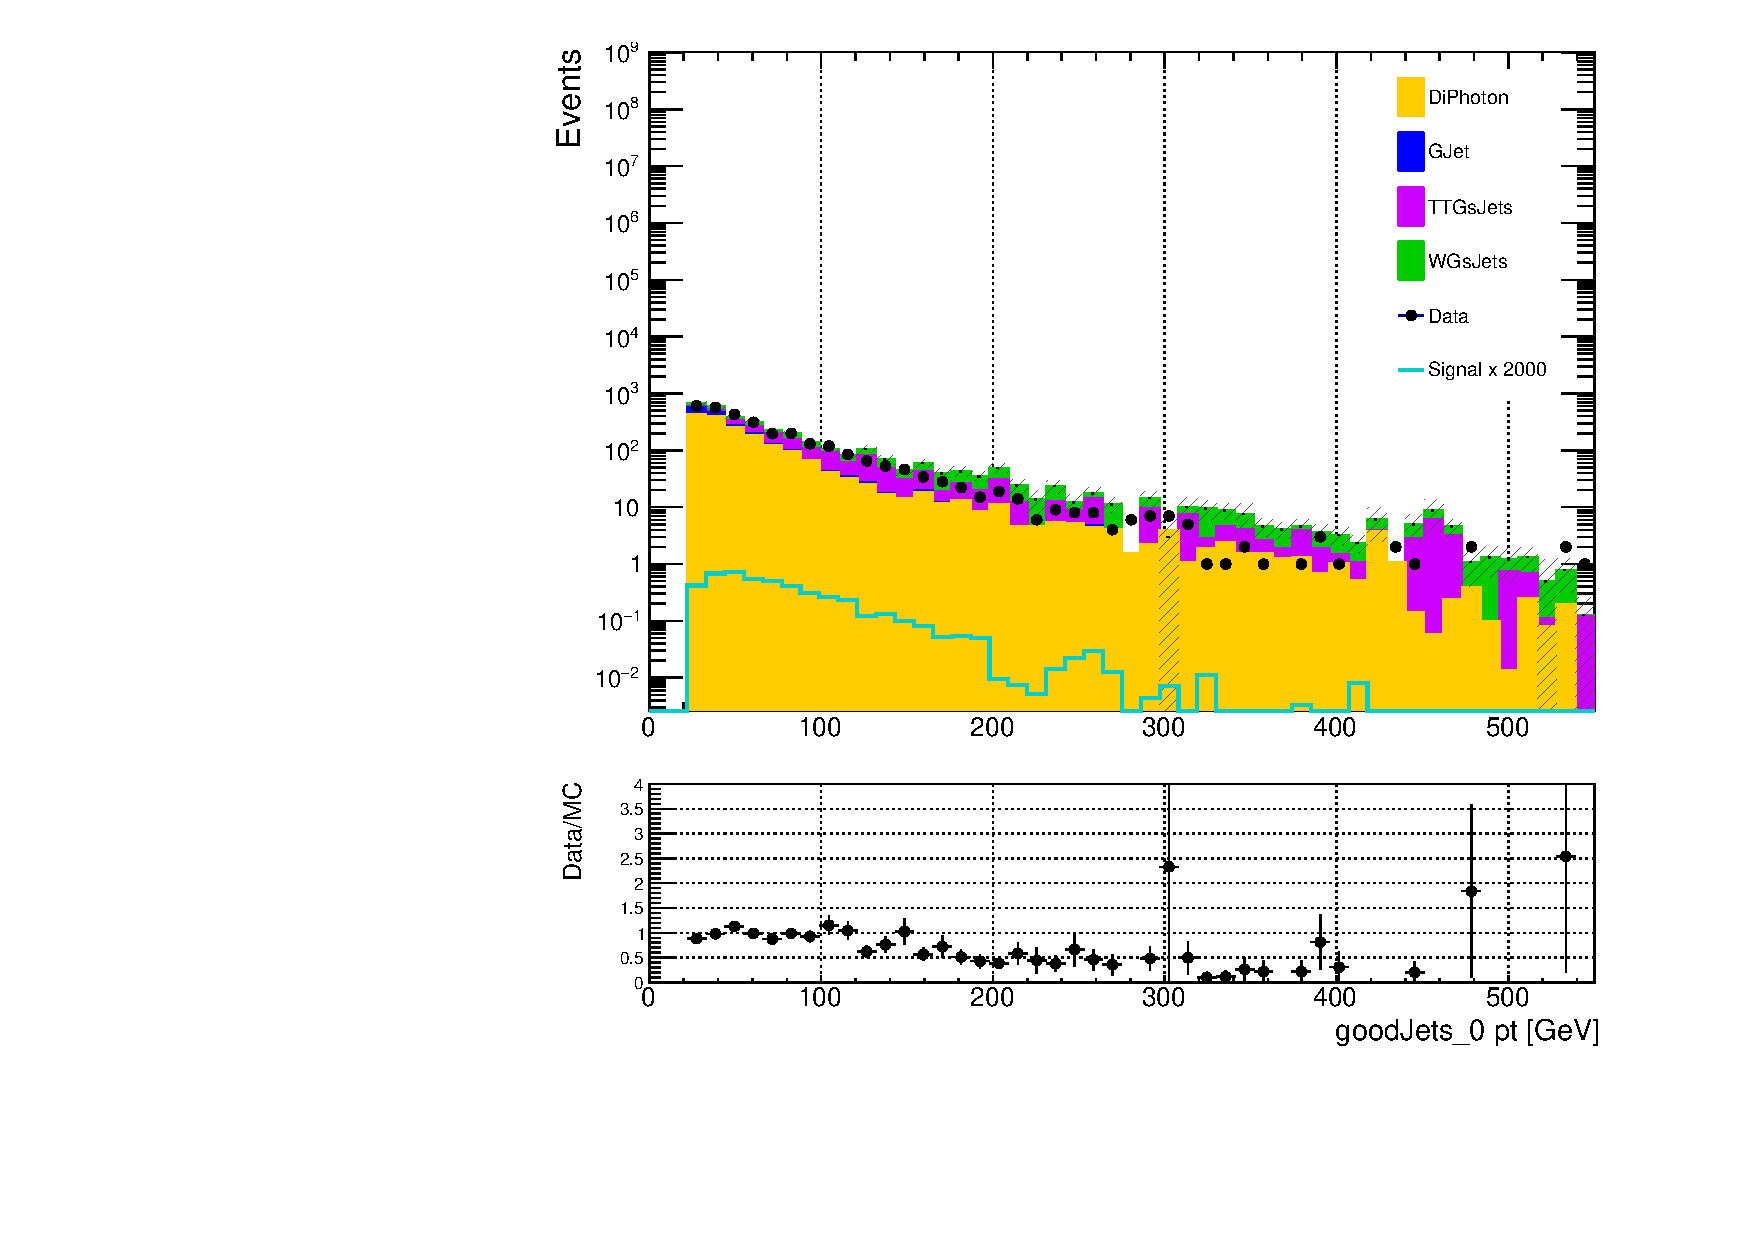
\includegraphics[width=0.45\textwidth]{Sections/HHWWgg/images/Semileptonic_Kinematic_Reweighting/Data_MC_WithKinWeights/goodJets_0_pt_log.pdf}\label{fig:Kin_Reweight_0_withKinWeights}}
    \caption{Leading jet \pt before and after kinematic reweighting (before any DNN evaluation), in the data sideband (100 $<$ $\mgg$ $<$ 115 or 135 $<$ $\mgg$ $<$ 180 GeV)}
    \label{fig:Kin_Reweight_0}
\end{figure} 

\begin{figure}[h!]
    \setcounter{subfigure}{0}
    \centering
    \subfloat[Before kinematic reweighting applied]{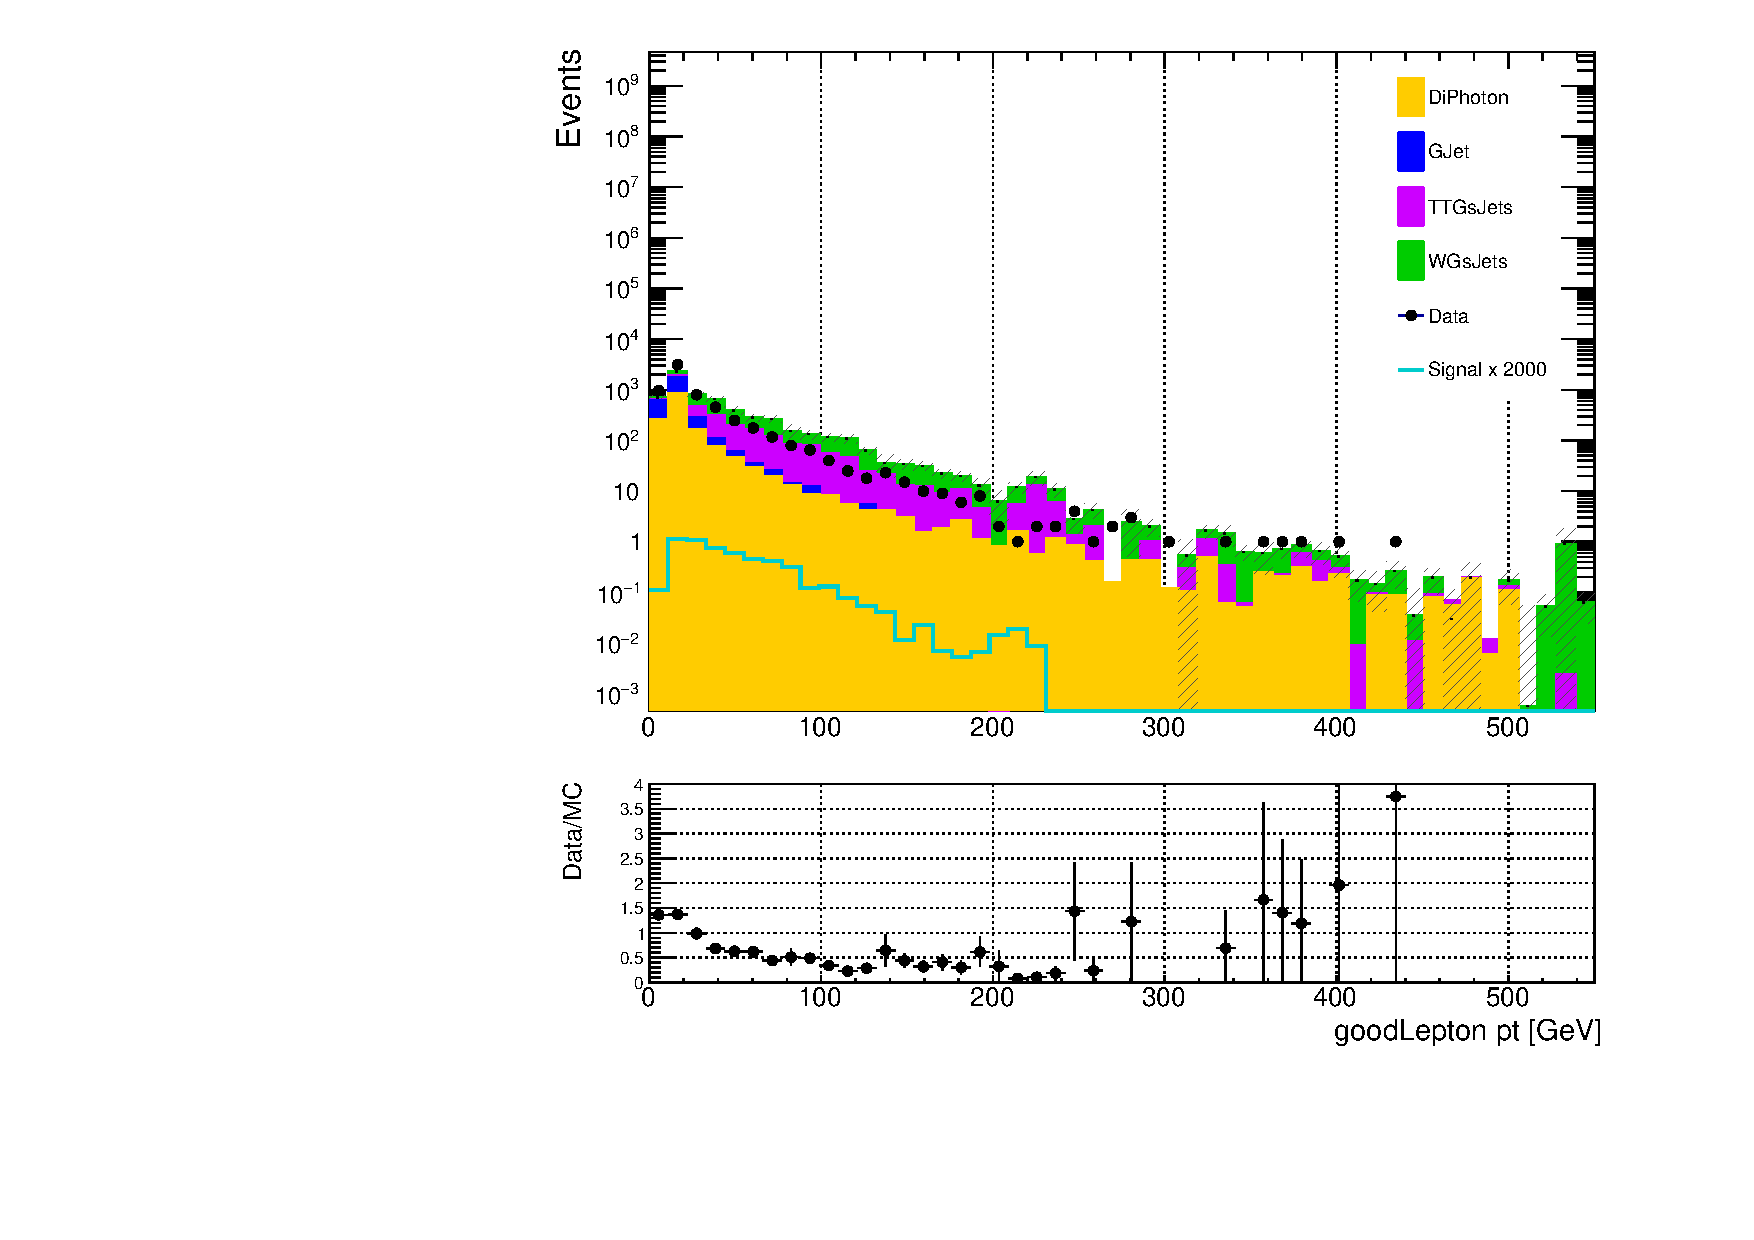
\includegraphics[width=0.45\textwidth]{Sections/HHWWgg/images/Semileptonic_Kinematic_Reweighting/Data_MC_WithoutKinWeights/goodLepton_pt_log.pdf}\label{fig:Kin_Reweight_1_withoutKinWeights}}
    \qquad
    \subfloat[After kinematic reweighting applied]{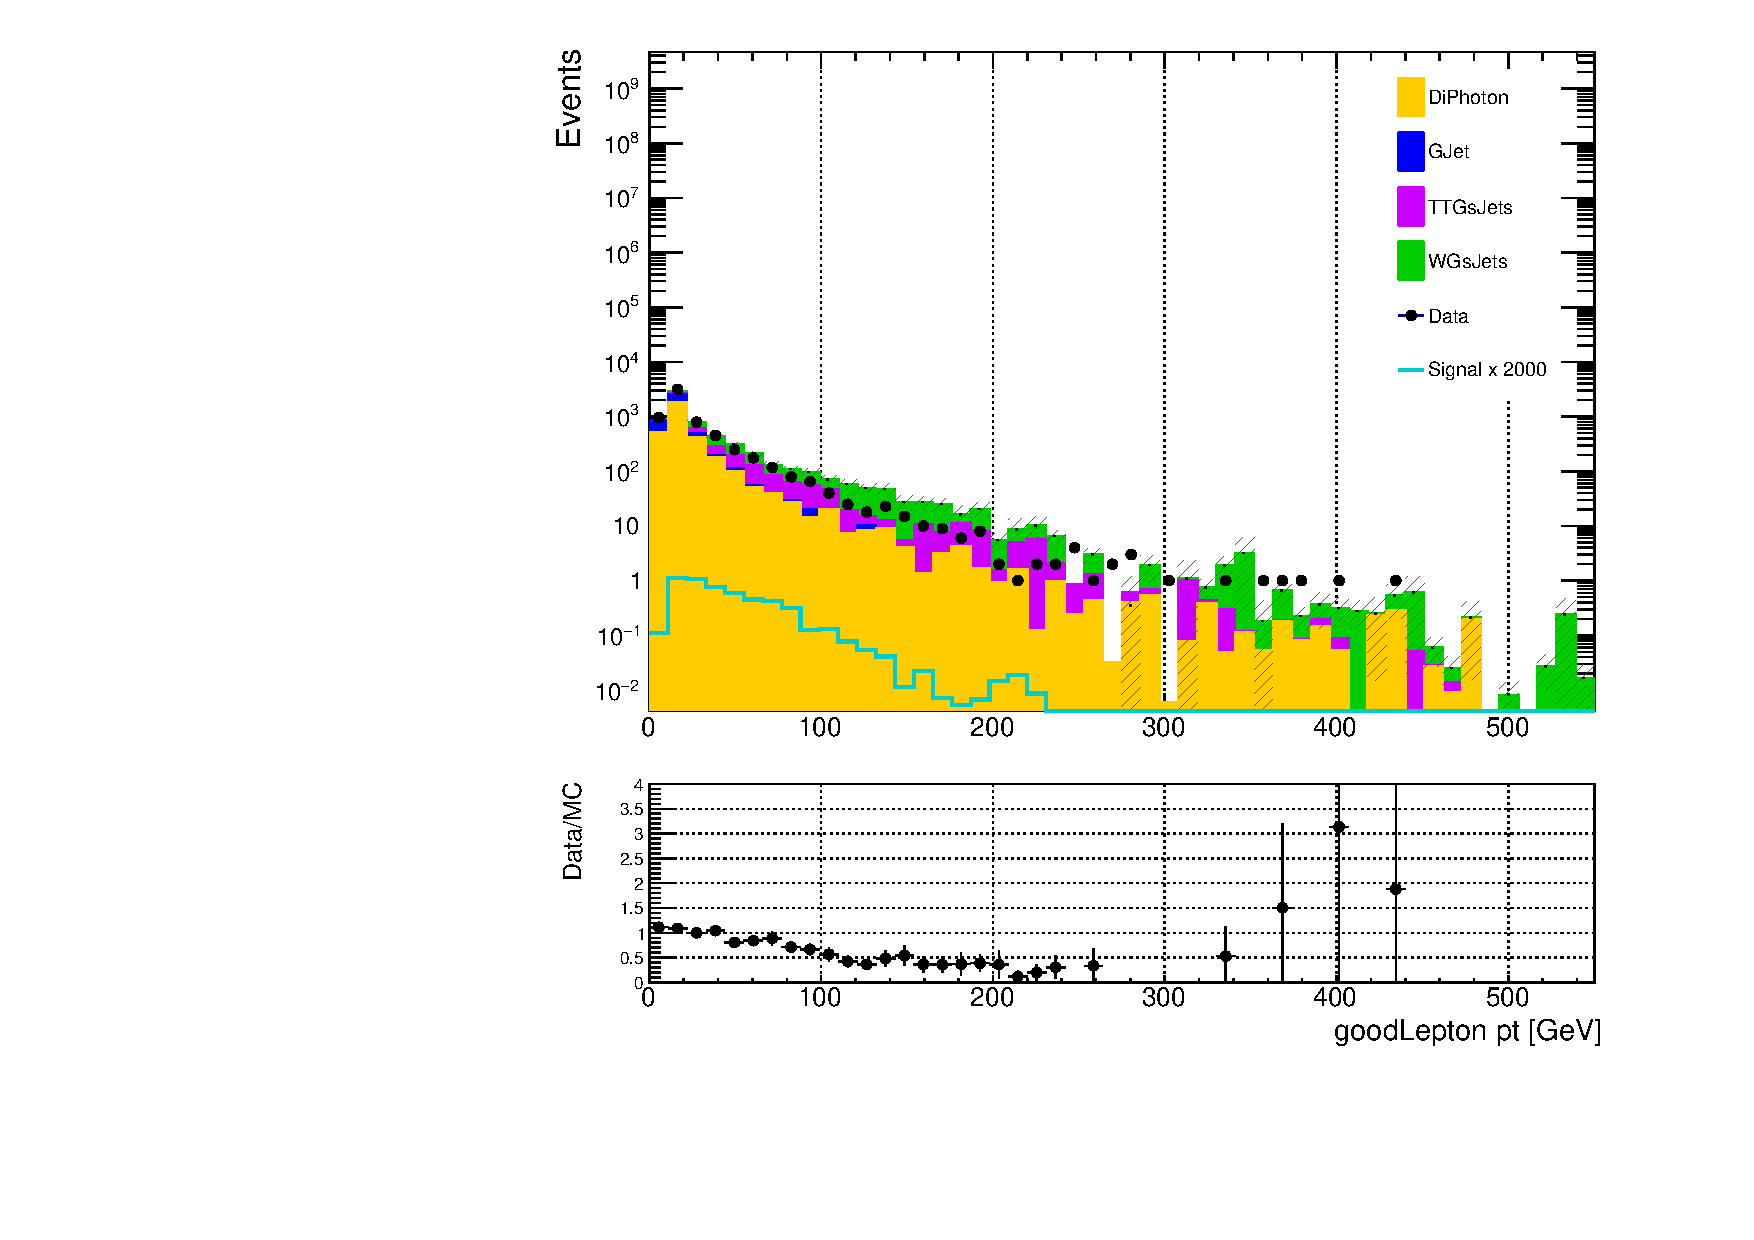
\includegraphics[width=0.45\textwidth]{Sections/HHWWgg/images/Semileptonic_Kinematic_Reweighting/Data_MC_WithKinWeights/goodLepton_pt_log.pdf}\label{fig:Kin_Reweight_1_withKinWeights}}
    \caption{Lepton \pt before and after kinematic reweighting (before any DNN evaluation), in the data sideband (100 $<$ $\mgg$ $<$ 115 or 135 $<$ $\mgg$ $<$ 180 GeV)}
    \label{fig:Kin_Reweight_2}
\end{figure} 

\begin{figure}[h!]
    \setcounter{subfigure}{0}
    \centering
    \subfloat[Before kinematic reweighting applied]{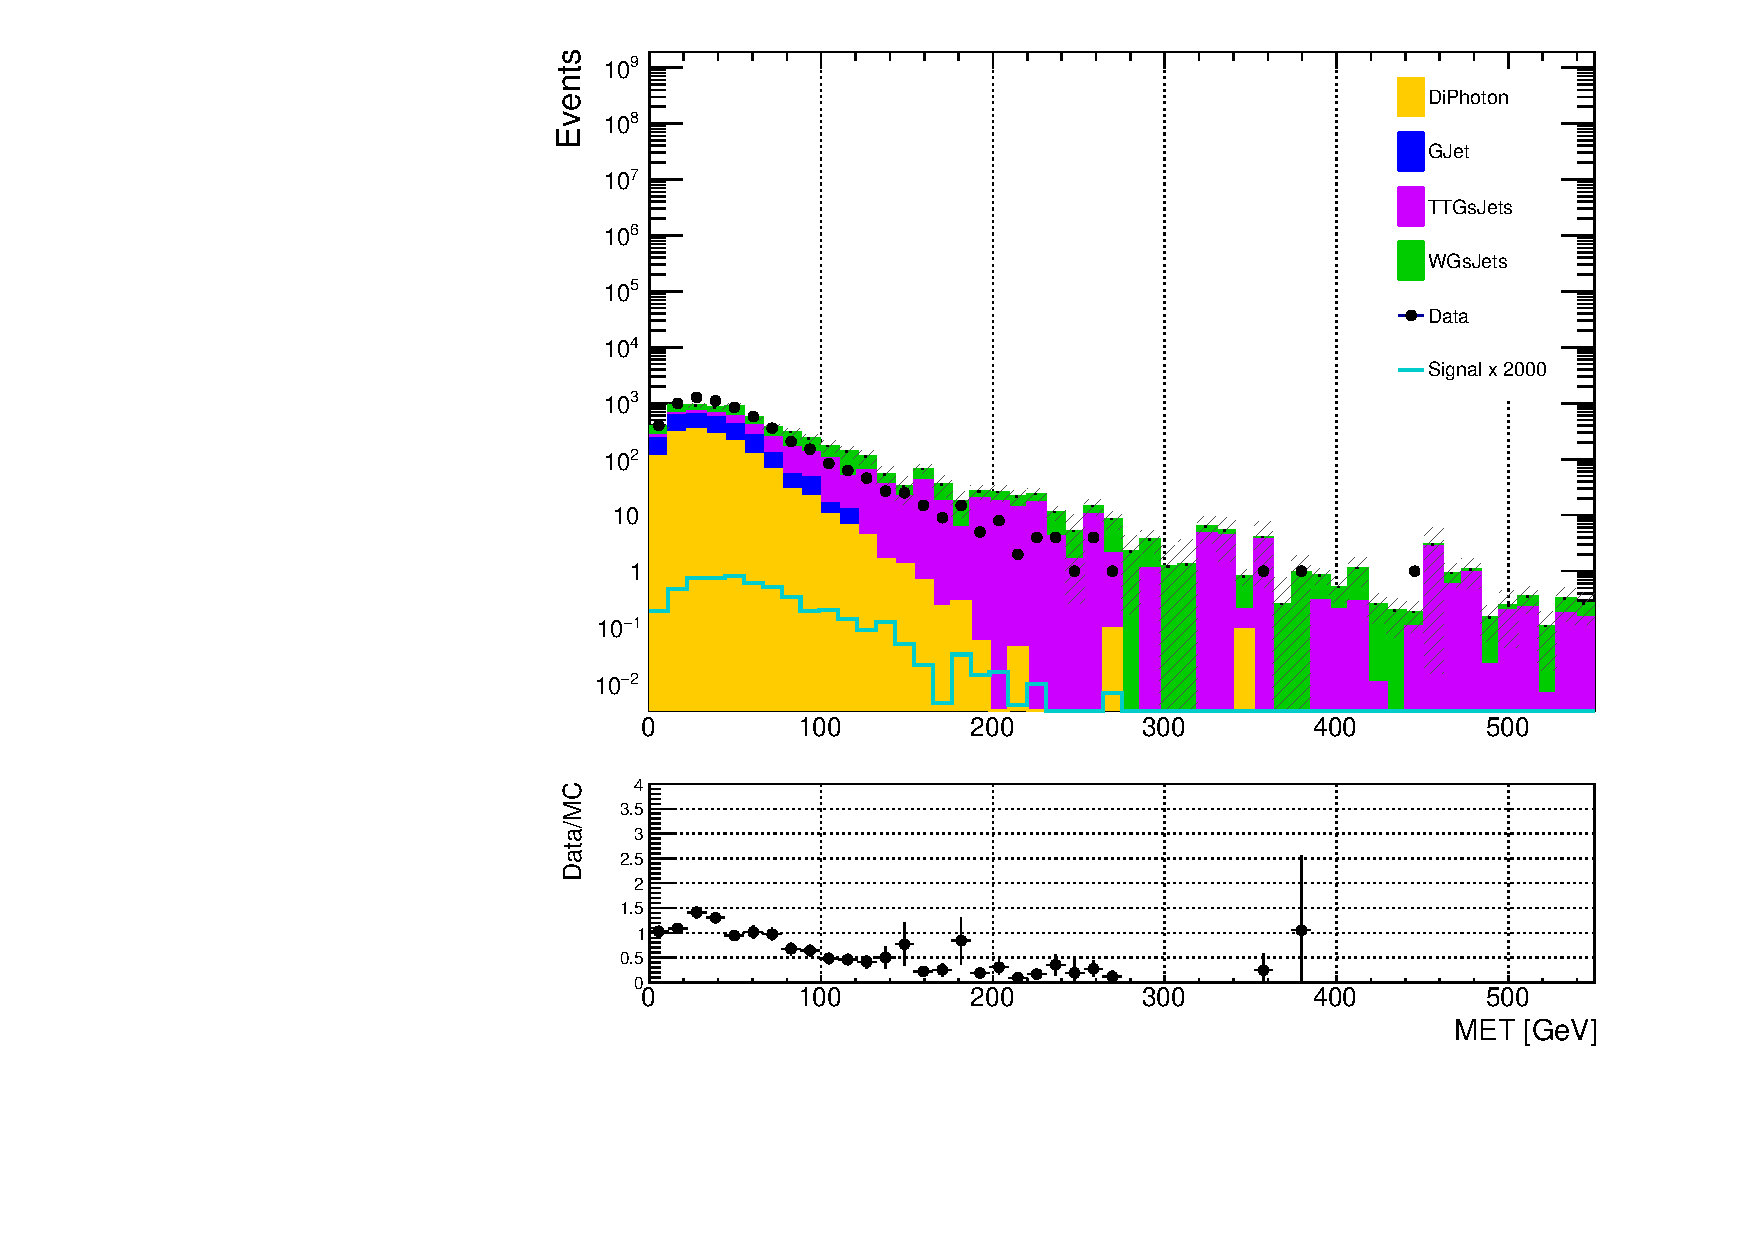
\includegraphics[width=0.45\textwidth]{Sections/HHWWgg/images/Semileptonic_Kinematic_Reweighting/Data_MC_WithoutKinWeights/MET_log.pdf}\label{fig:Kin_Reweight_2_withoutKinWeights}}
    \qquad
    \subfloat[After kinematic reweighting applied]{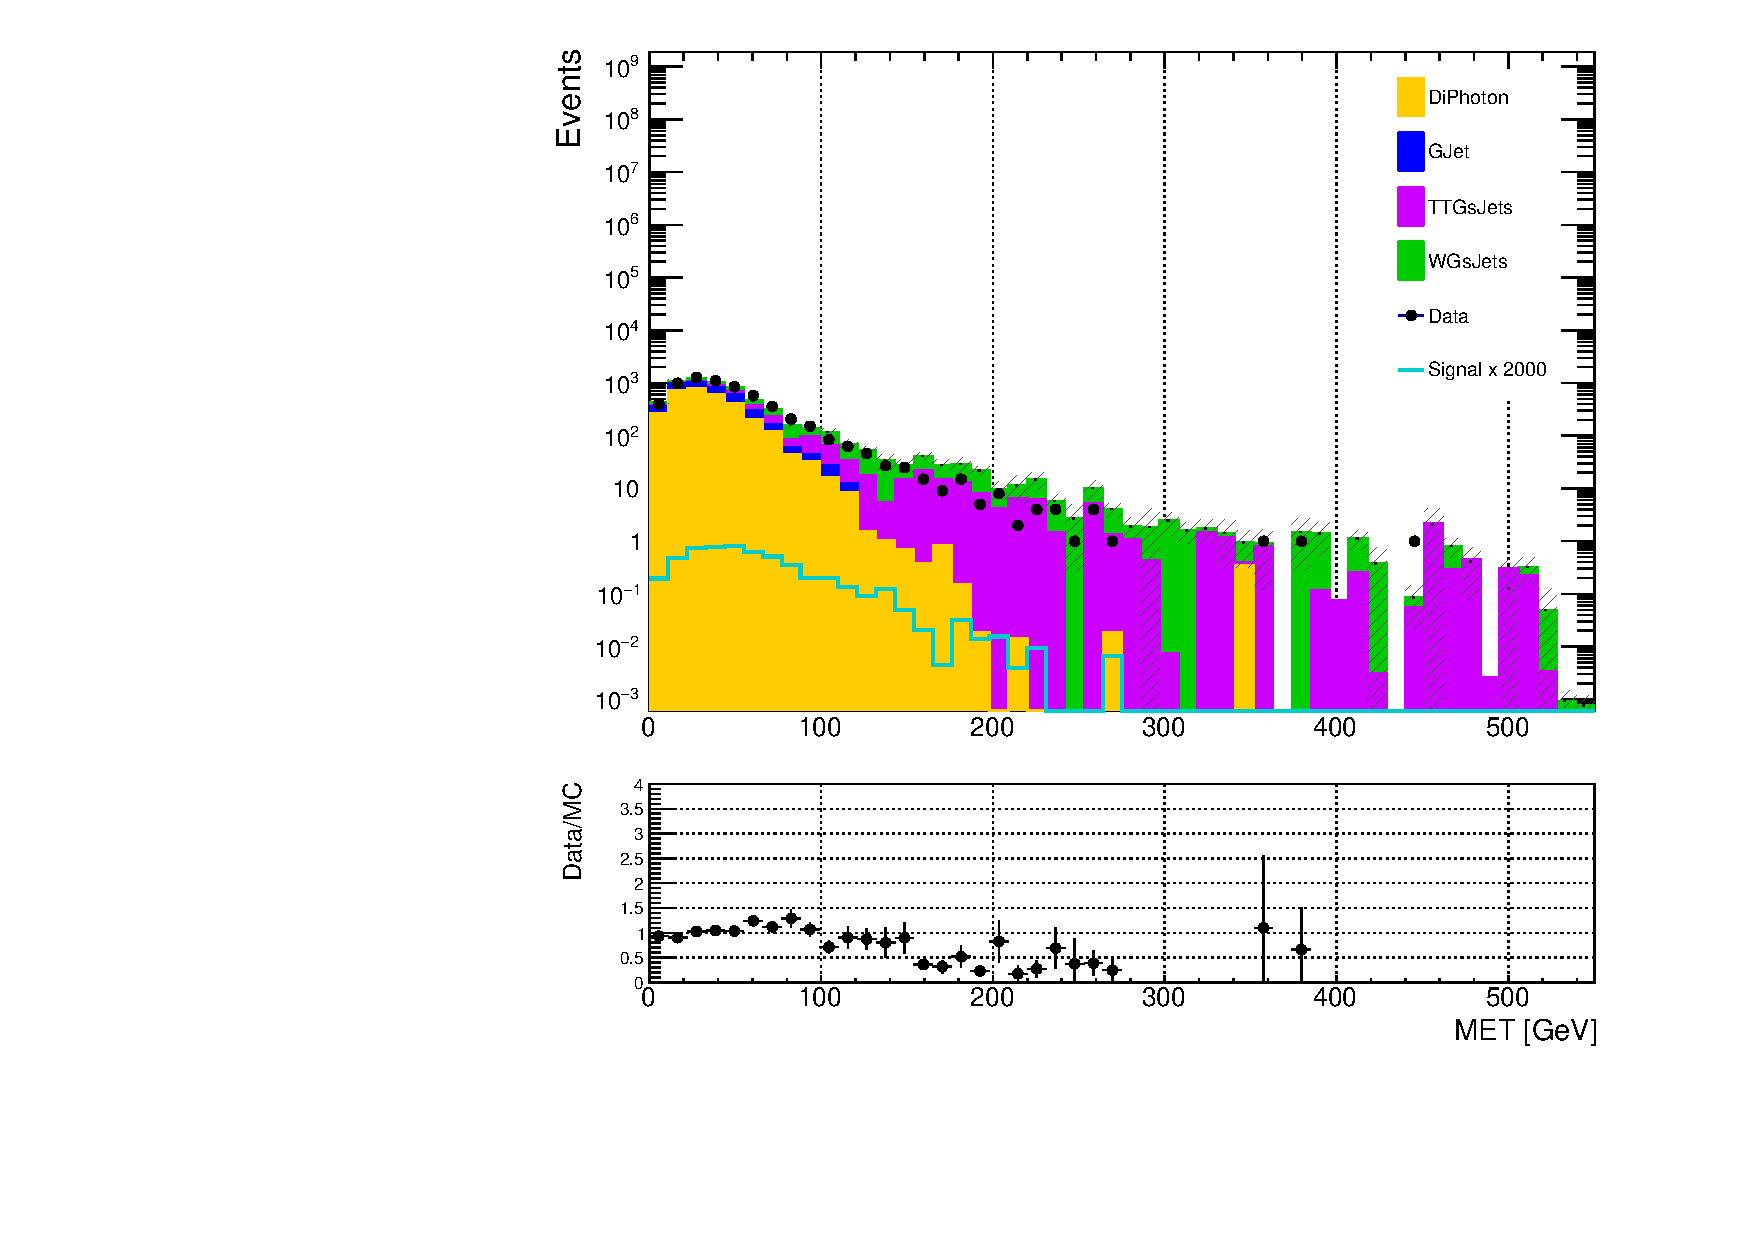
\includegraphics[width=0.45\textwidth]{Sections/HHWWgg/images/Semileptonic_Kinematic_Reweighting/Data_MC_WithKinWeights/MET_log.pdf}\label{fig:Kin_Reweight_2_withKinWeights}}
    \caption{MET before and after kinematic reweighting (before any DNN evaluation), in the data sideband (100 $<$ $\mgg$ $<$ 115 or 135 $<$ $\mgg$ $<$ 180 GeV)}
    \label{fig:Kin_Reweight_3}
\end{figure} 
  
\begin{figure}[h!]
    \setcounter{subfigure}{0}
    \centering
    \subfloat[Before kinematic reweighting applied]{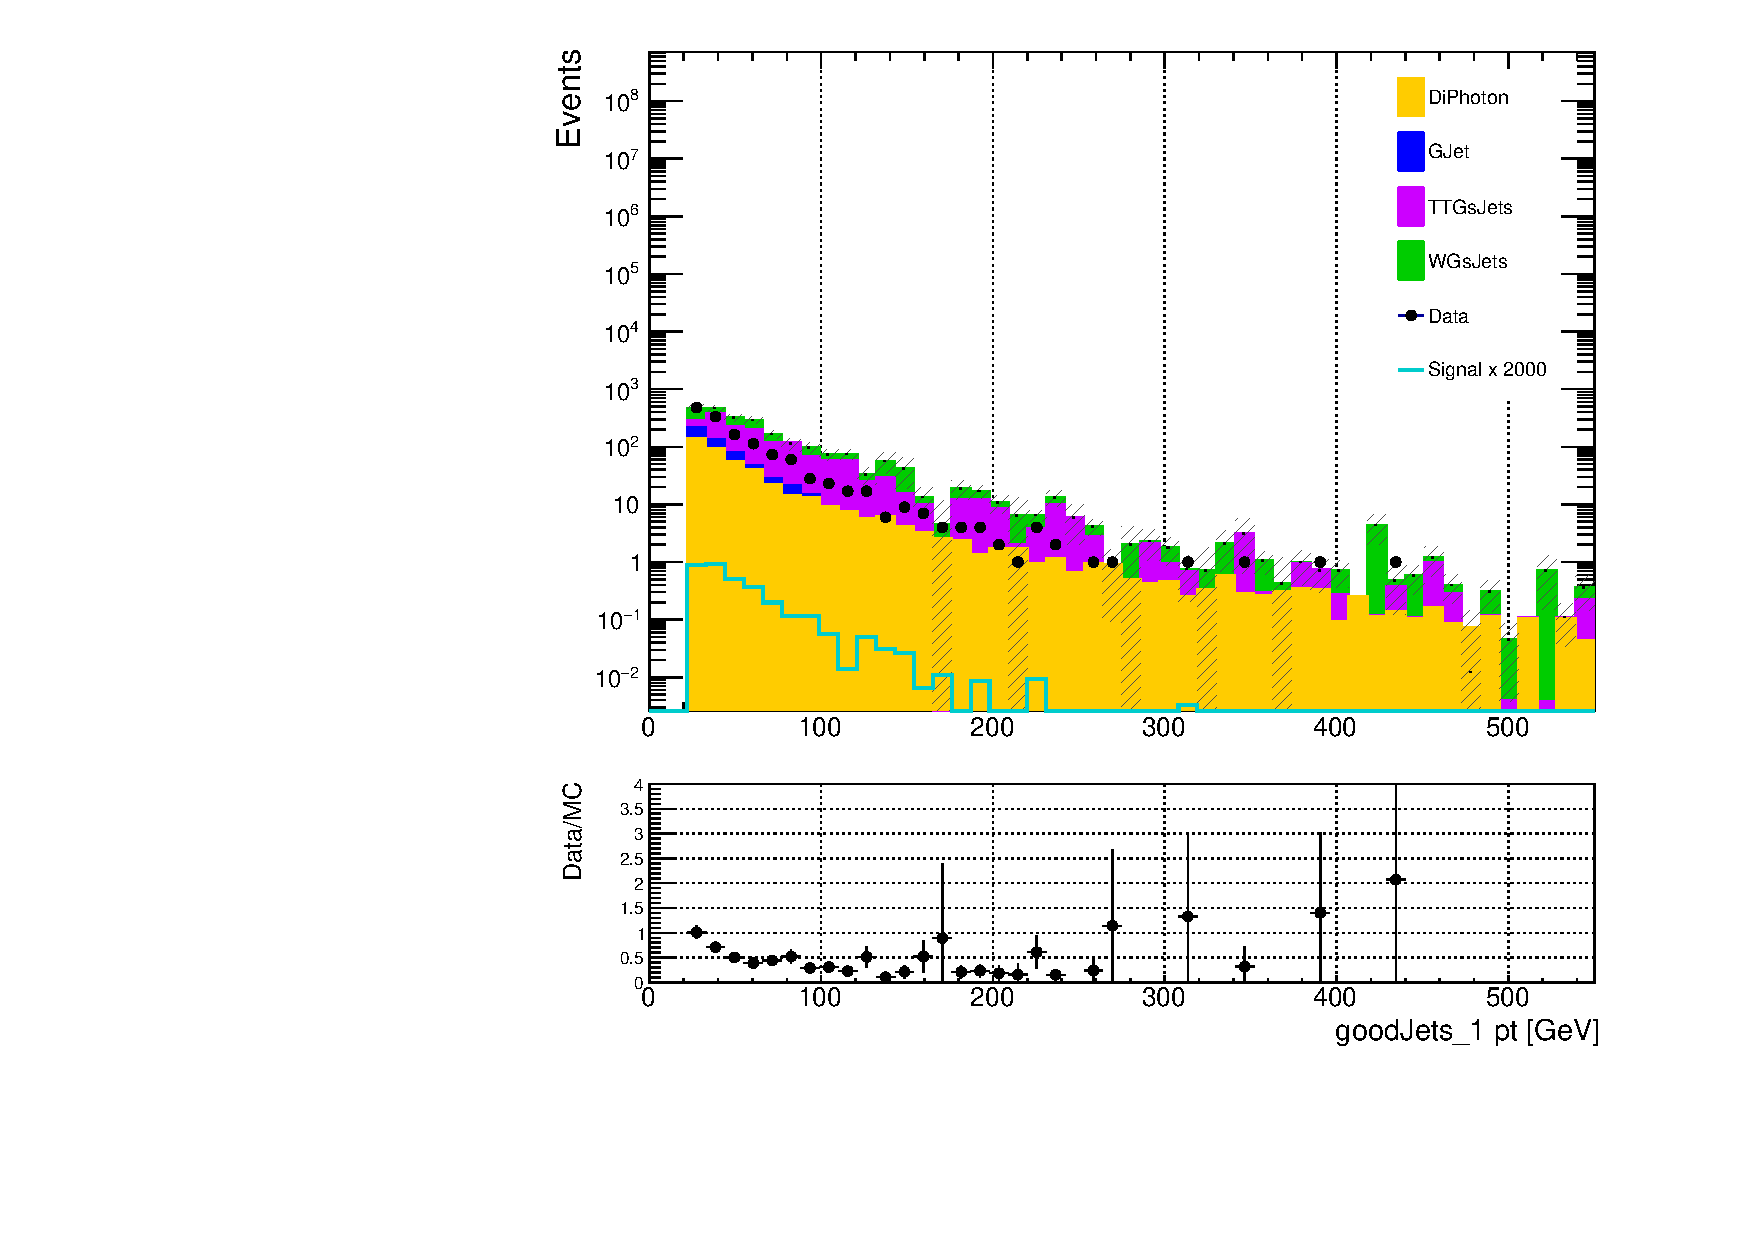
\includegraphics[width=0.45\textwidth]{Sections/HHWWgg/images/Semileptonic_Kinematic_Reweighting/Data_MC_WithoutKinWeights/goodJets_1_pt_log.pdf}\label{fig:Kin_Reweight_3_withoutKinWeights}}
    \qquad
    \subfloat[After kinematic reweighting applied]{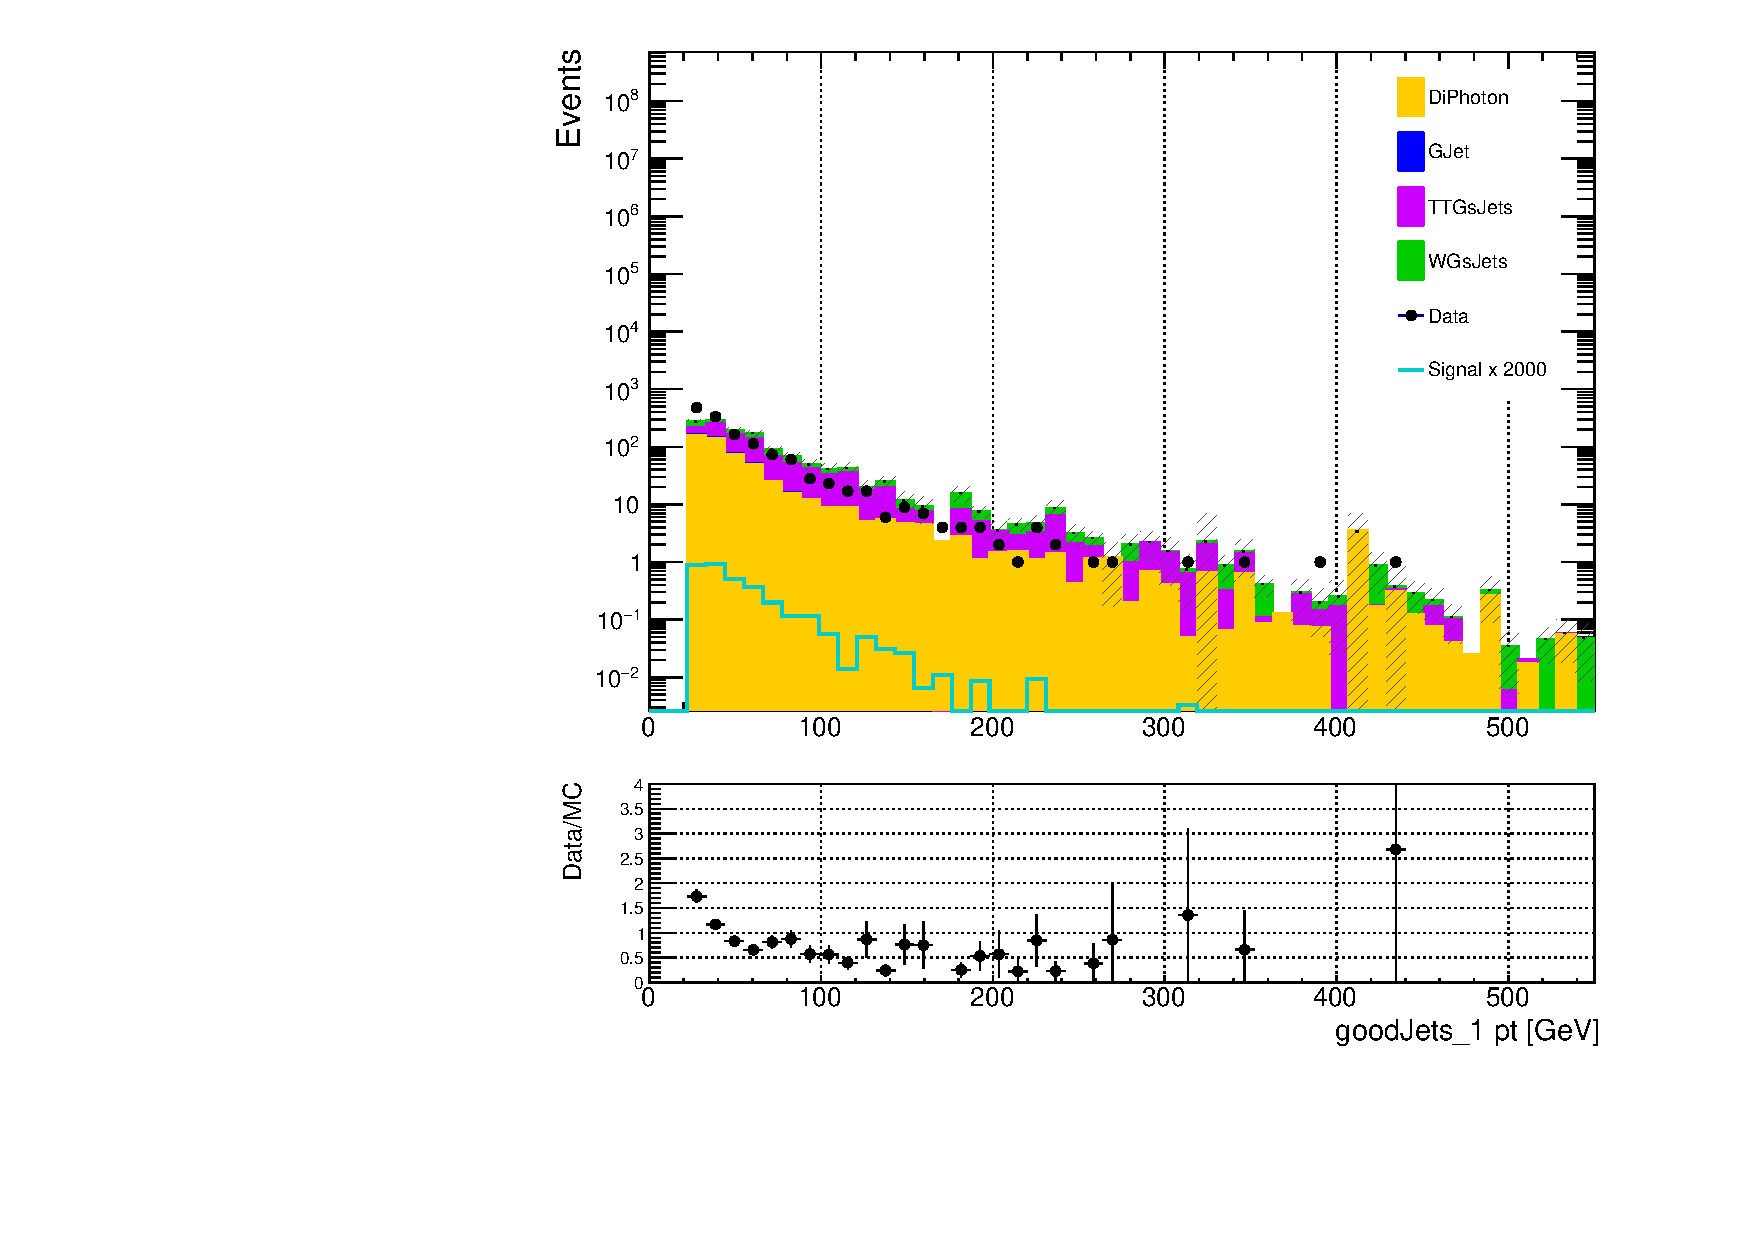
\includegraphics[width=0.45\textwidth]{Sections/HHWWgg/images/Semileptonic_Kinematic_Reweighting/Data_MC_WithKinWeights/goodJets_1_pt_log.pdf}\label{fig:Kin_Reweight_3_withKinWeights}}
    \caption{Subleading jet \pt before and after kinematic reweighting (before any DNN evaluation), in the data sideband (100 $<$ $\mgg$ $<$ 115 or 135 $<$ $\mgg$ $<$ 180 GeV)}
    \label{fig:Kin_Reweight_1}
\end{figure} 

\begin{figure}[h!]
    \setcounter{subfigure}{0}
    \centering
    \subfloat[Before kinematic reweighting applied]{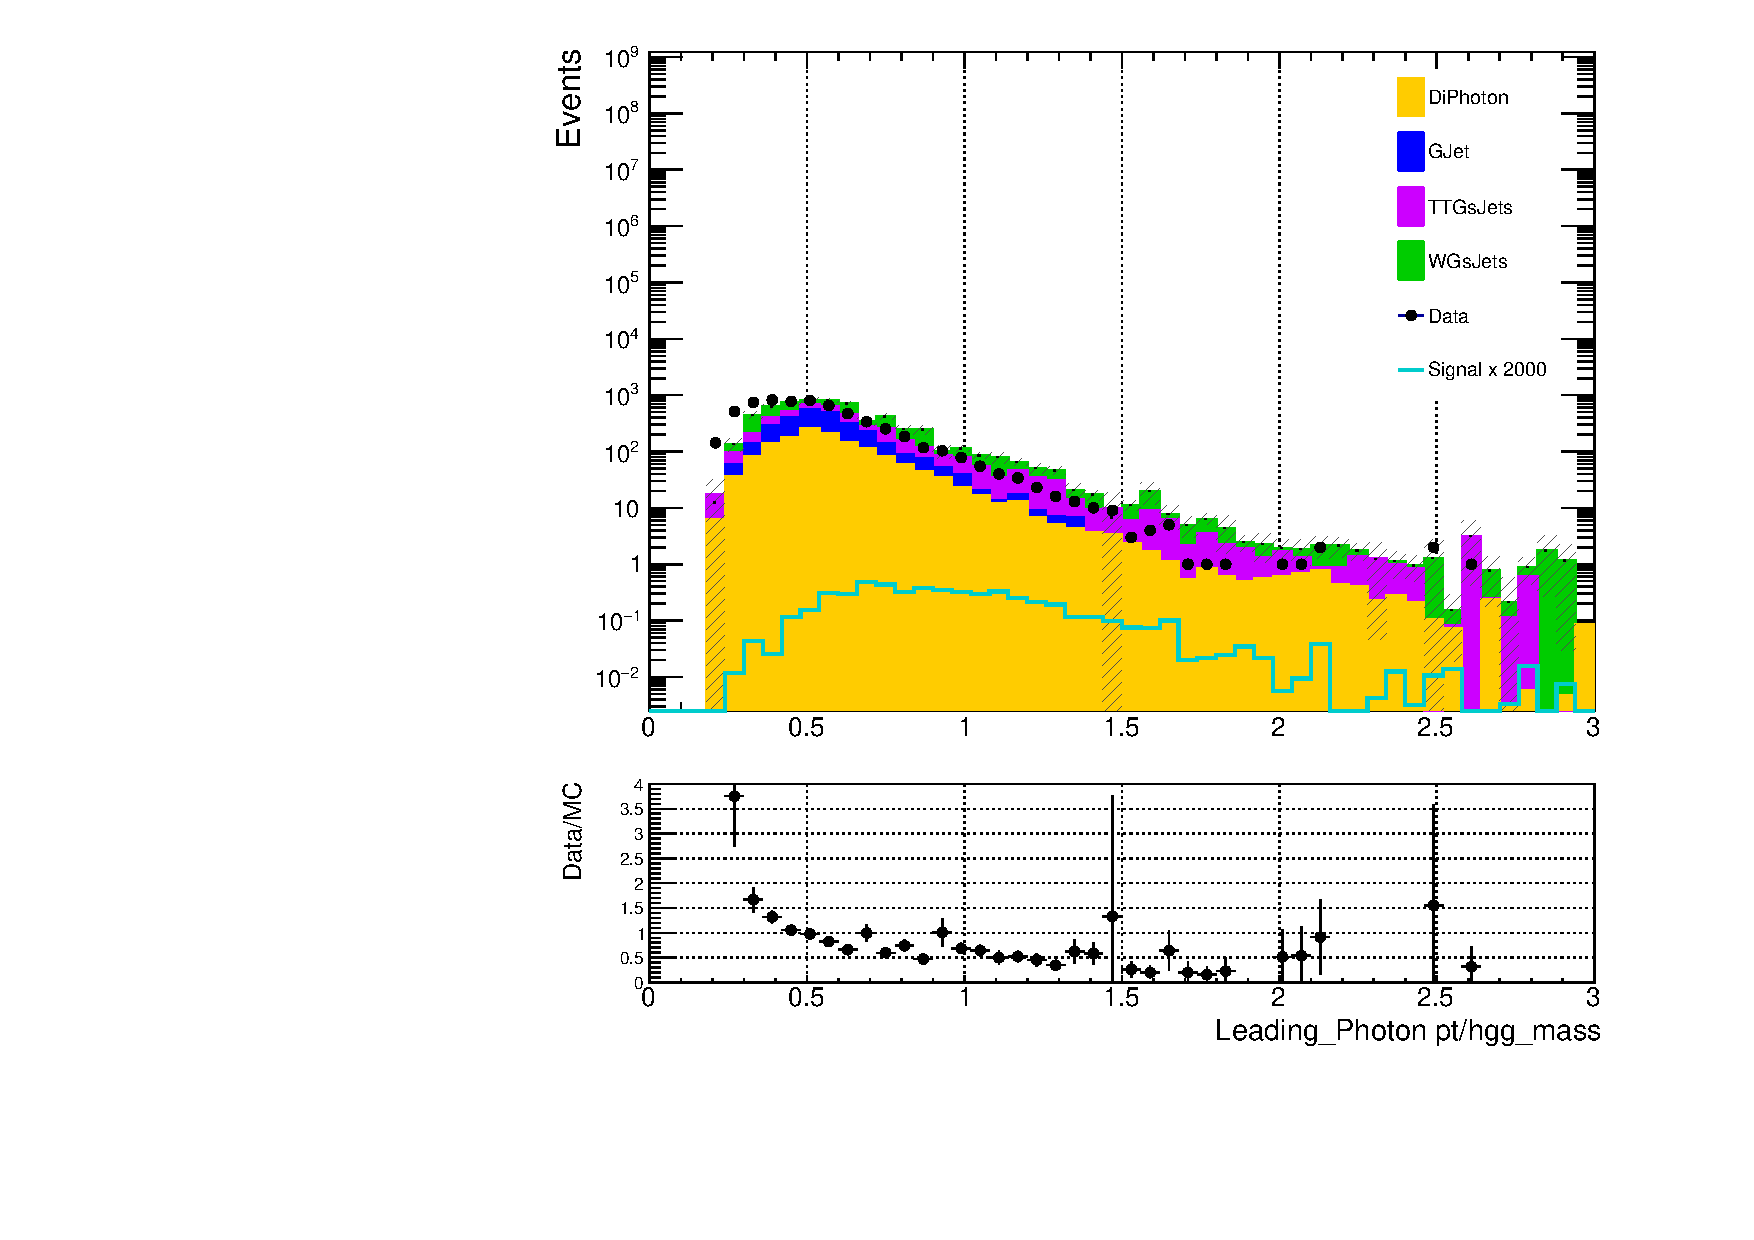
\includegraphics[width=0.45\textwidth]{Sections/HHWWgg/images/Semileptonic_Kinematic_Reweighting/Data_MC_WithoutKinWeights/Leading_Photon_pt_over_CMS_hgg_mass_log.pdf}\label{fig:Kin_Reweight_4_withoutKinWeights}}
    \qquad
    \subfloat[After kinematic reweighting applied]{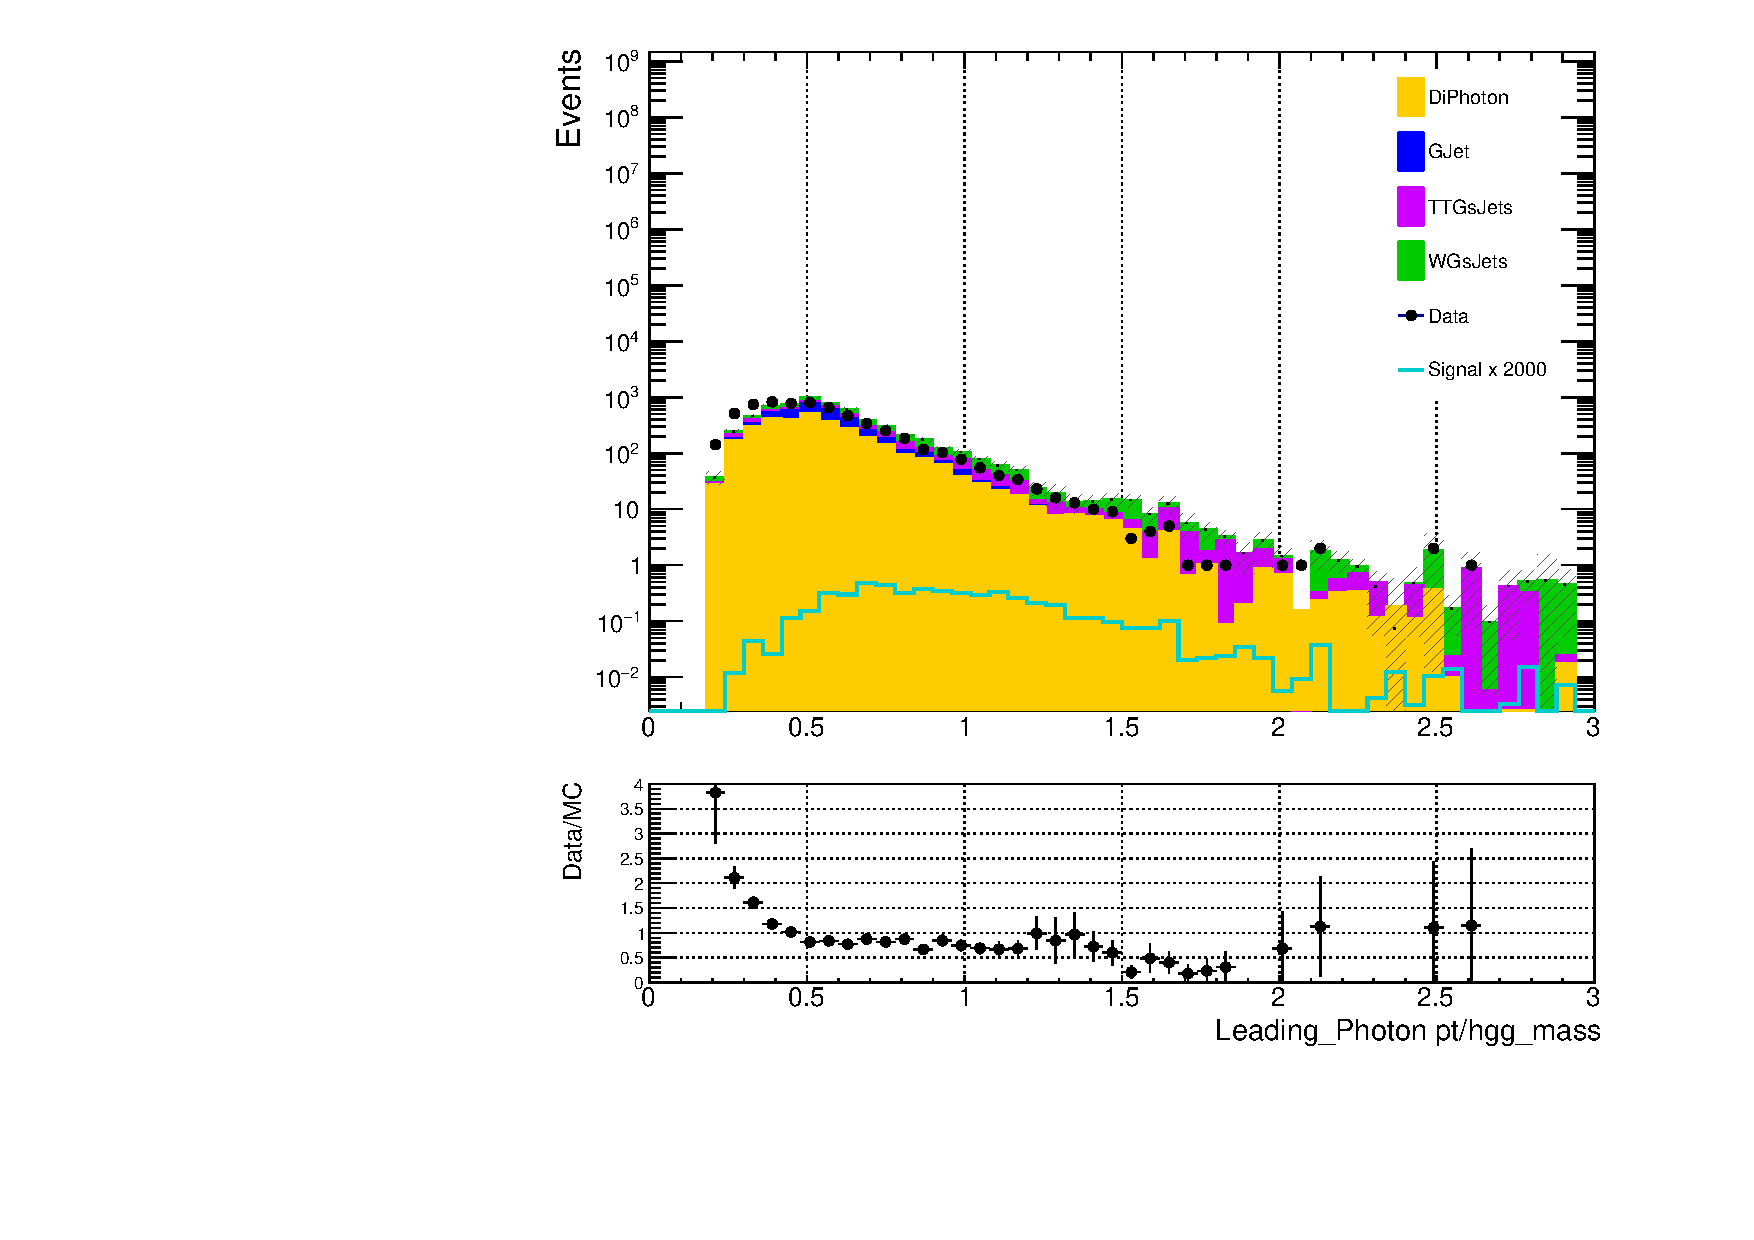
\includegraphics[width=0.45\textwidth]{Sections/HHWWgg/images/Semileptonic_Kinematic_Reweighting/Data_MC_WithKinWeights/Leading_Photon_pt_over_CMS_hgg_mass_log.pdf}\label{fig:Kin_Reweight_4_withKinWeights}}
    \caption{Leading photon \pt over \mgg before and after kinematic reweighting (before any DNN evaluation), in the data sideband (100 $<$ $\mgg$ $<$ 115 or 135 $<$ $\mgg$ $<$ 180 GeV)}
    \label{fig:Kin_Reweight_4}
\end{figure} 

\begin{figure}[h!]
    \setcounter{subfigure}{0}
    \centering
    \subfloat[Before kinematic reweighting applied]{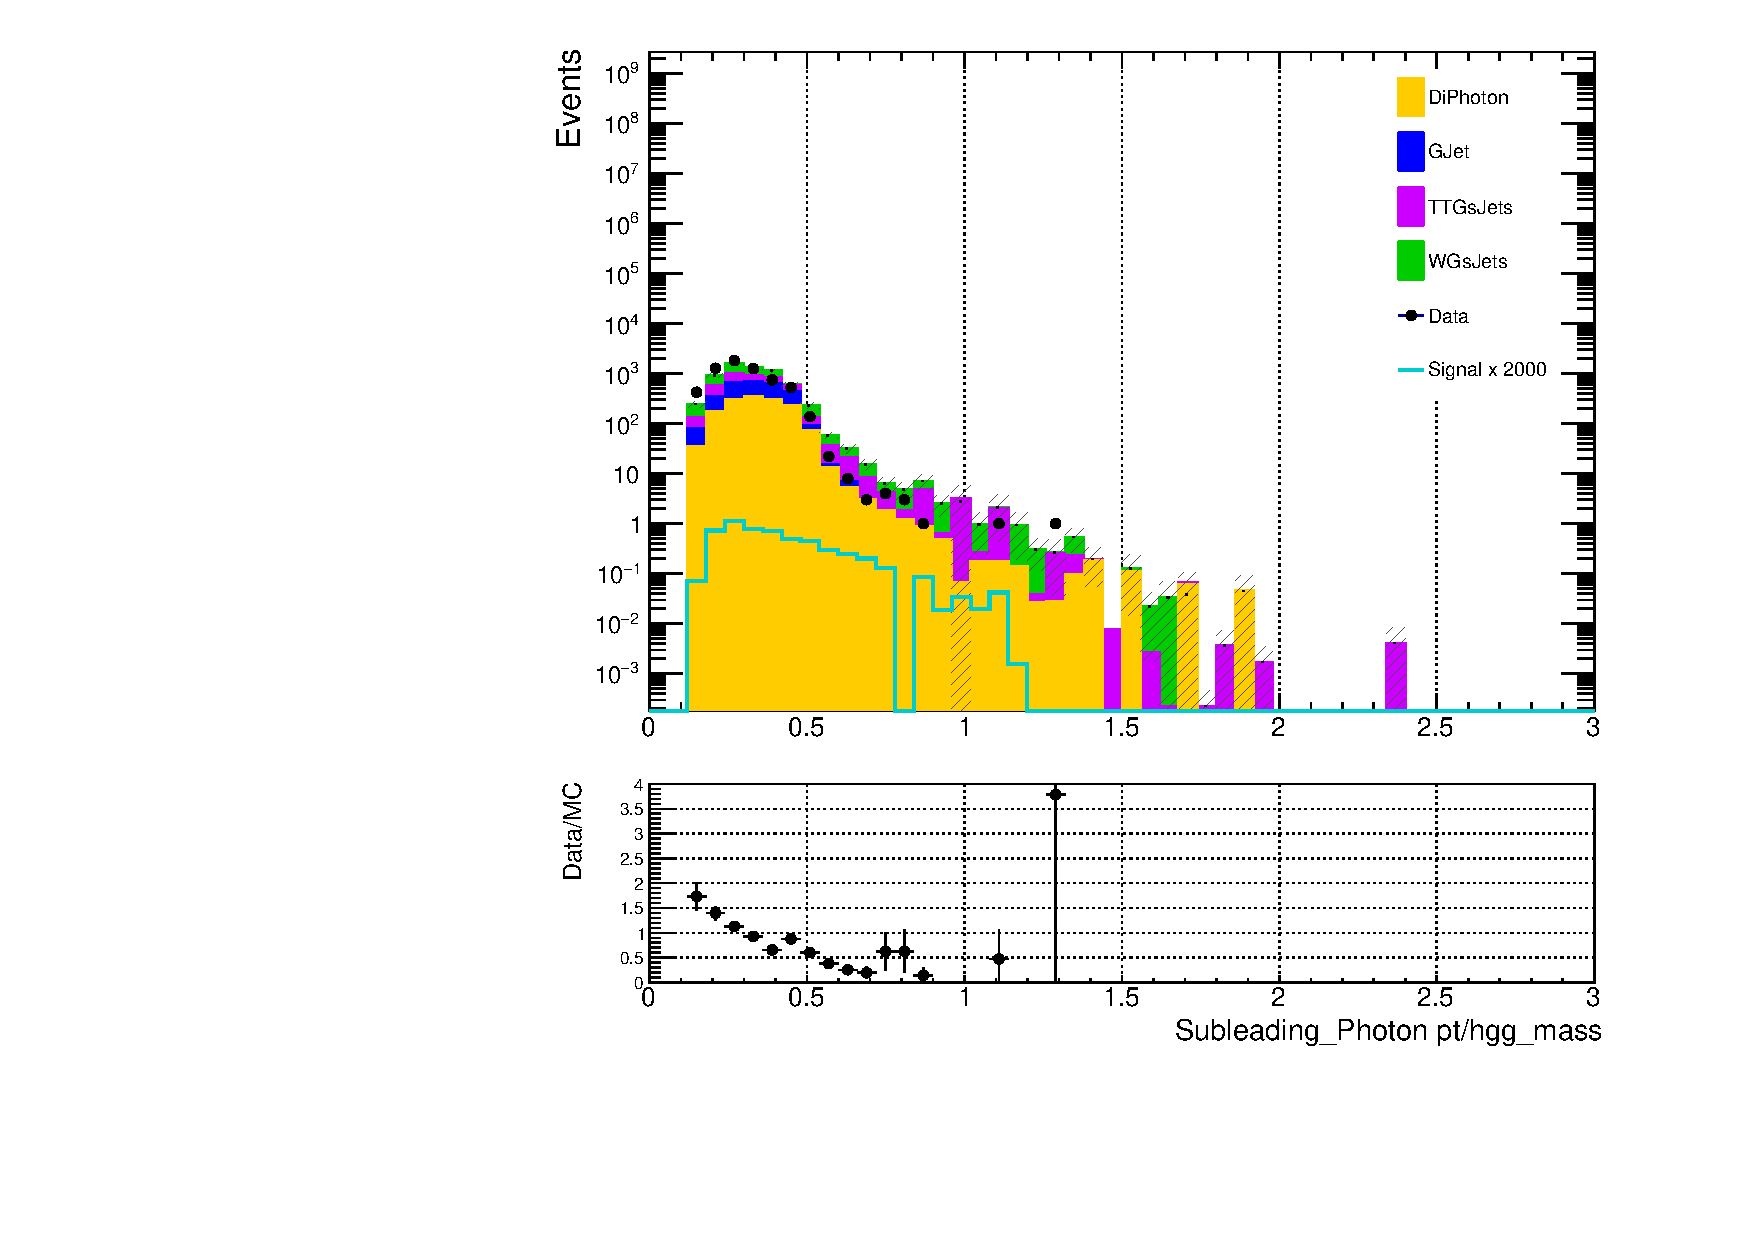
\includegraphics[width=0.45\textwidth]{Sections/HHWWgg/images/Semileptonic_Kinematic_Reweighting/Data_MC_WithoutKinWeights/Subleading_Photon_pt_over_CMS_hgg_mass_log.pdf}\label{fig:Kin_Reweight_5_withoutKinWeights}}
    \qquad
    \subfloat[After kinematic reweighting applied]{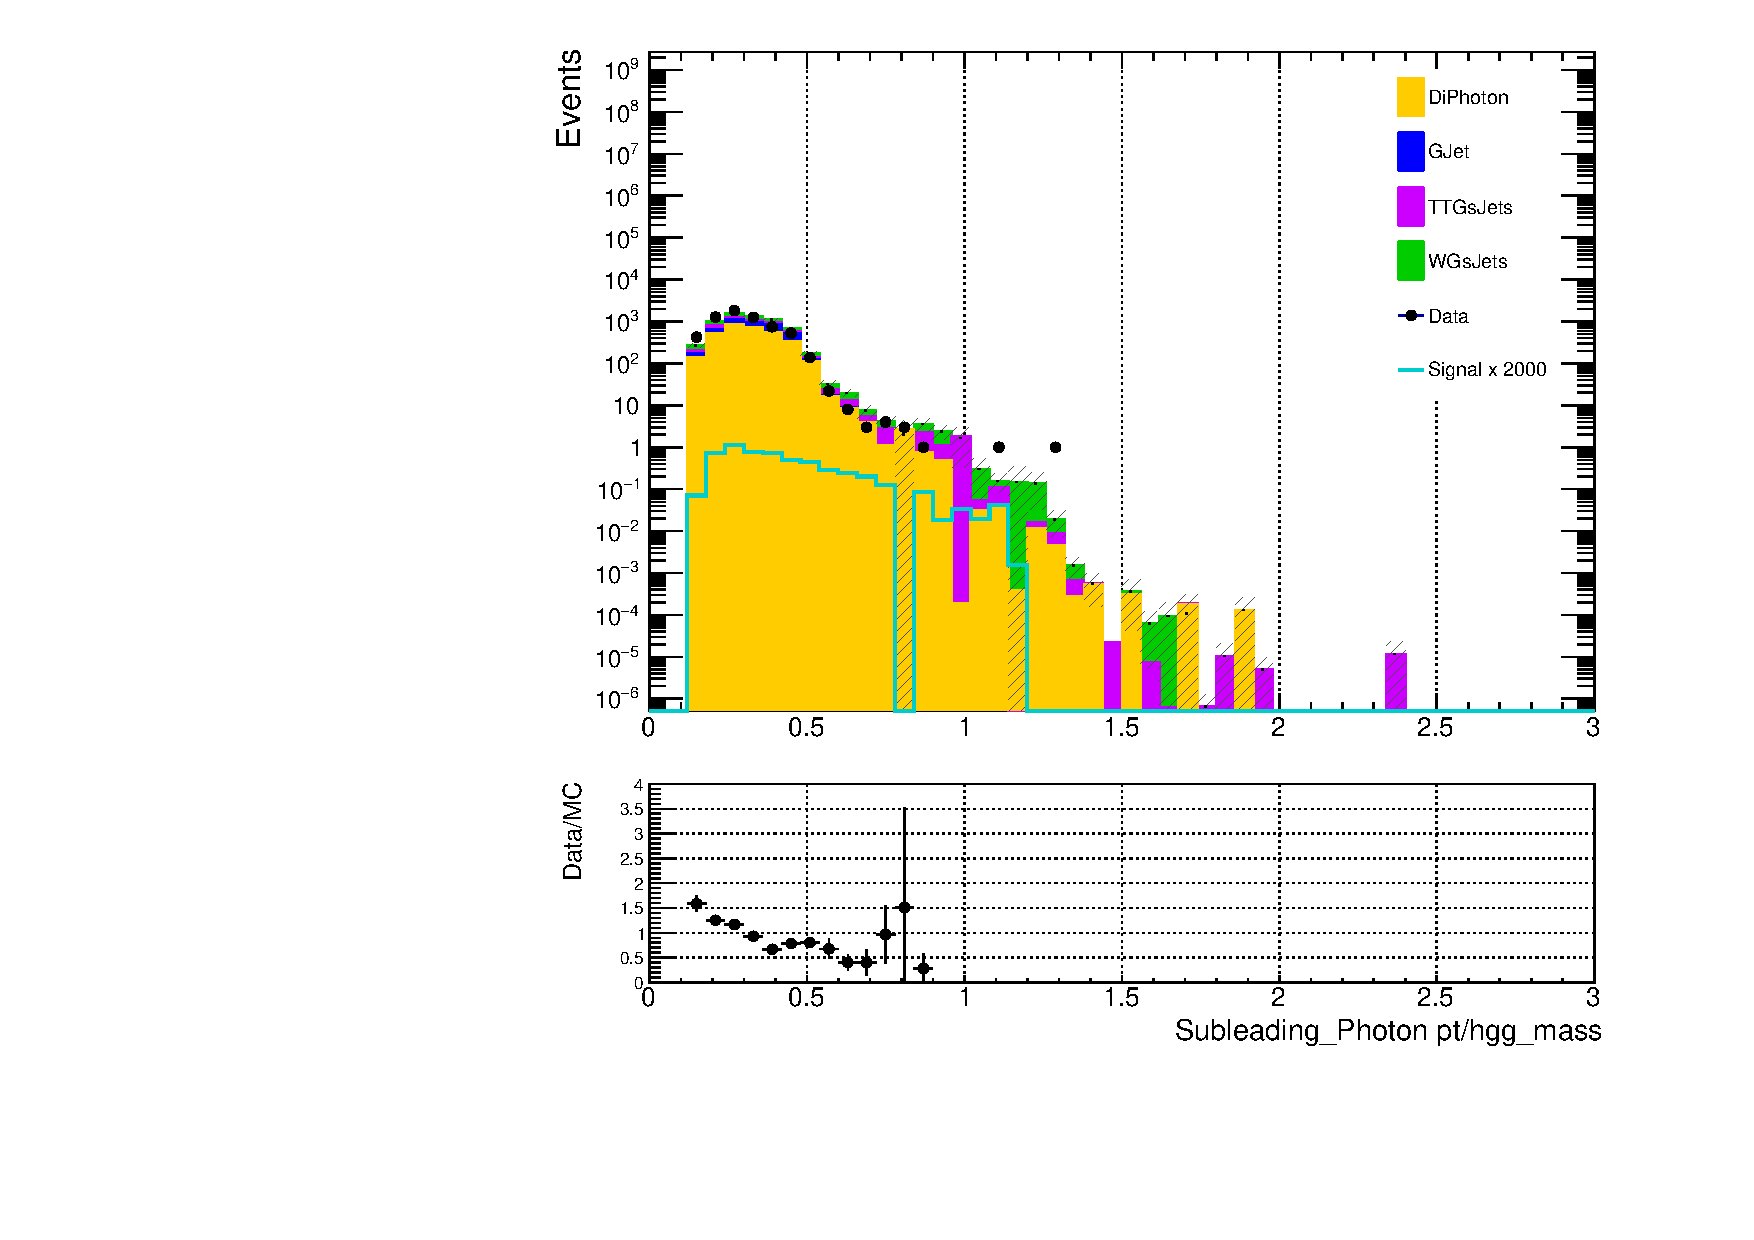
\includegraphics[width=0.45\textwidth]{Sections/HHWWgg/images/Semileptonic_Kinematic_Reweighting/Data_MC_WithKinWeights/Subleading_Photon_pt_over_CMS_hgg_mass_log.pdf}\label{fig:Kin_Reweight_5_withKinWeights}}
    \caption{Subleading photon \pt over \mgg before and after kinematic reweighting (before any DNN evaluation), in the data sideband (100 $<$ $\mgg$ $<$ 115 or 135 $<$ $\mgg$ $<$ 180 GeV)}
    \label{fig:Kin_Reweight_5}
\end{figure} 

\clearpage 

The MultiClass DNN outputs three DNN scores, each with a range 0-1 and corresponding to the likelihood that an event falls into each of the three classes, which sum to one. This means that if an event has a high 
HH class DNN score, the sum of the H and continuum background DNN scores must be small. Because of this constraint, only the output HH class DNN score is used in the analysis for categorization as 
it has a known correlation to the output H and continuum background DNN scores. 

The DNN training results in the ROC (Receiver operating curve) shown in Figure \ref{fig:ROC_HH}, and normalized DNN scores for the three classes shown in Figure \ref{fig:SL_DNN_overfitting_check}.

A possible way to improve this analysis in the future would be to make use of the H and continuum background DNN scores, for instance in order to define control regions with high H and continuum background but low HH yields. These could potentially be included in the simultaneous fit to data in order to decrease the statistical uncertainty, and improve the modelling of the single Higgs templates in the signal region.  

Due to the non-linearity of deep neural network models, understanding the relative importance of the input features is non-trivial. In this analysis,
we evaluate the relative importance by evaluating Shapley values \cite{shapley_values} for each feature. The Shapley value is the average of the marginal
contribution of a feature's value to the prediction, across all possible coalitions of features. Specifically, it is calculated by taking the difference in the
value of the prediction with and without a given feature (the marginal contribution). This is repeated for all possible combinations of the other input features and
the average value of the marginal contributions is taken as the Shapely value. It is important to note that the Shapley value is the average contribution of a feature
value to the prediction in the different coalitions of features and not the difference in prediction with and without the feature in the model. 
It is also worth noting that coalitions of features can be formed without the complete list of input features. When this happens, in order to
evaluate the network the missing feature(s) value is randomised in order to obtain a prediction. The relative importance of the input features can be found in
Figure \ref{fig:SLfeatureranking_HH}, for the HH class DNN score. The variables are
ranked from highest to lowest in order of their discriminatory power per class. The leading importance variables all correspond to quantities from the final state topology of the semi-leptonic WW$\gamma\gamma$ process, namely two photons, one lepton, two jets and a neutrino.

\begin{figure}[H]
  \setcounter{subfigure}{0}
  \centering
  \subfloat[All Shapley scores]{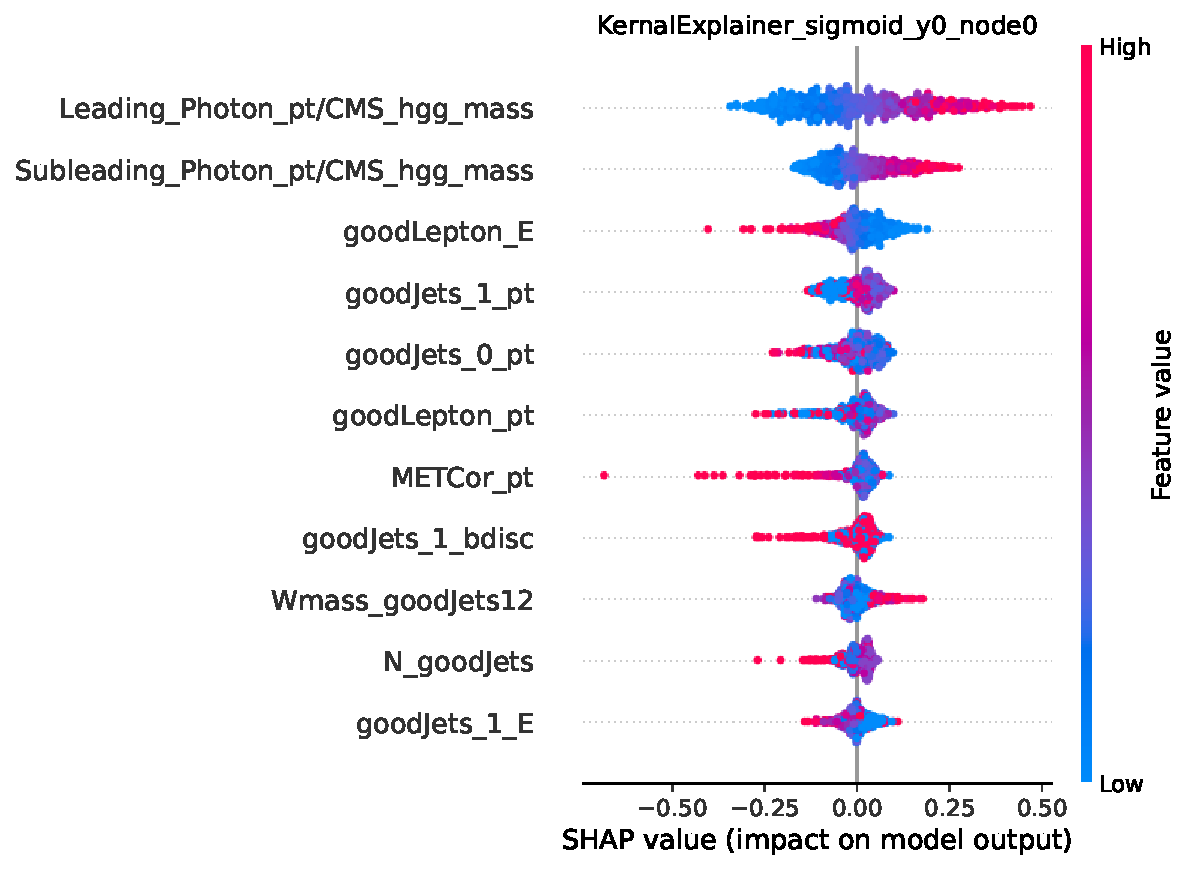
\includegraphics[width=0.45\textwidth]{Sections/HHWWgg/images/DNN/KernalExplainer_sigmoid_y0_node0.pdf}}
  %\qquad
  \subfloat[Average Shapley score magnitudes]{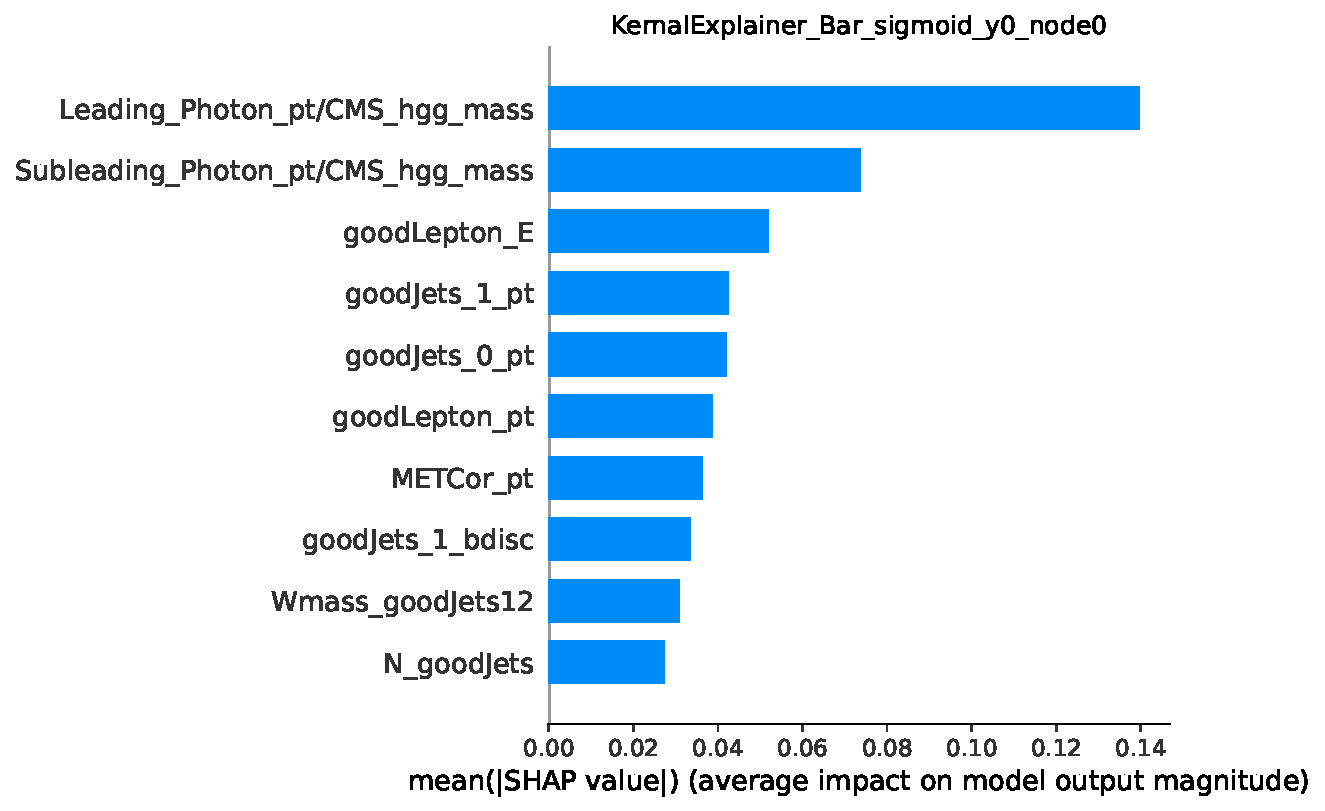
\includegraphics[width=0.45\textwidth]{Sections/HHWWgg/images/DNN/KernalExplainer_Bar_sigmoid_y0_node0.pdf}}
  \caption{Semi-leptonic channel DNN input feature ranking according to Shapely values in the HH class}
  \label{fig:SLfeatureranking_HH}
\end{figure} 

\begin{figure}[H]
  \setlength{\unitlength}{1mm}
  \begin{center}
    \mbox{\includegraphics*[height=100mm]{Sections/HHWWgg/images/DNN/MultiClass_ROC_class_HH.pdf}
    }
  \end{center}
  \caption{Semi-Leptonic DNN ROC curve for training and test data: HH Class}
  \label{fig:ROC_HH}
\end{figure}

\begin{figure}[H]
  \setlength{\unitlength}{1mm}
  \begin{center}
    \mbox{\includegraphics*[height=100mm]{Sections/HHWWgg/images/DNN/overfitting_plot_HH_Non-Categorised.pdf}
    }
  \end{center}
  \caption{Normalized HH DNN score distributions for the three semileptonic DNN nodes, shown for training and test events.}
  \label{fig:SL_DNN_overfitting_check}
\end{figure}

% Data/MC after training:

% A single sideband weight is extracted and applied in order to compare the data and MC shapes. 

% The sideband weight is obtained and shapre comparison performed
% in the follow way: MC is scaled to the ratio of data / MC integrals
% in the sidebands, 

% of the di-photon mass in the data sidebands with and without this sideband weight value of 1.140 is shown in 
% Figure \ref{fig:DNNSidebands_withAndWithoutSidebandScale}.

Events with a DNN score less than 0.1 are removed and not used for categorization, nor in any background or signal modelling, as this region is largely background dominant. 

In order to qualitatively understand the level of optimization of the DNN in identifying data events with MC, the data / MC ratio comparison of events with a DNN score greater than 0.1 are shown for the leading importance input variables in Figures \ref{fig:SLDNNFeaturecontrolplots-1} and \ref{fig:SLDNNFeaturecontrolplots-2}. It should be noted 
that any disagreement between data and MC will lead to a sub-optimal network, but will not introduce any bias in the final result extraction, as MC is only used for selection and categorization optimization. 

% The data-MC ratio of all remaining input variables can be found in Appendix \ref{sec:DNN-Input-Variables}.

Table \ref{tab:SL_DNN_Background_yields} shows the post-selection yields, including a selection on the output DNN score of $>$ 0.1, for all of the simulated samples
used in this analysis, both the absolute number and the corresponding yield accounting for proper MC scaling.

The correlation plot of all input features can also be found in Figure \ref{fig:inputvarcorrelation} and is used to check if any correlations are present between input training variables. In particular it can 
be seen there is less than 2\% correlation between all input variables and reconstructed diphoton mass, ``CMS$\_$hgg$\_$mass", indicating that a bias in diphoton mass distributions is 
not expected. Note that the diphoton mass variable is only included in the correlation 
matrix in order to ensure the DNN does not train on any input features correlated to the signal region, as the diphoton mass is not included in the training. 

An additional check is 
performed to ensure the resulting DNN does not shape the diphoton mass, outlined in Appendix \ref{sec:SL_DNN_Sideband_Check}. No evident shaping is seen, and therefore no bias is expected from the DNN. In addition,
a check is performed in a dedicated control region to demonstrate that a large difference in data and MC acceptance is not expected to be introduced by the DNN, and that the DNN behaves as expected on its target signal topology. This check is shown in Appendix \ref{sec:DNN_and_signal_validation}. 

\begin{figure}[H]
\setcounter{subfigure}{0}
\centering
\subfloat[Scaled Leading Photon \pt]{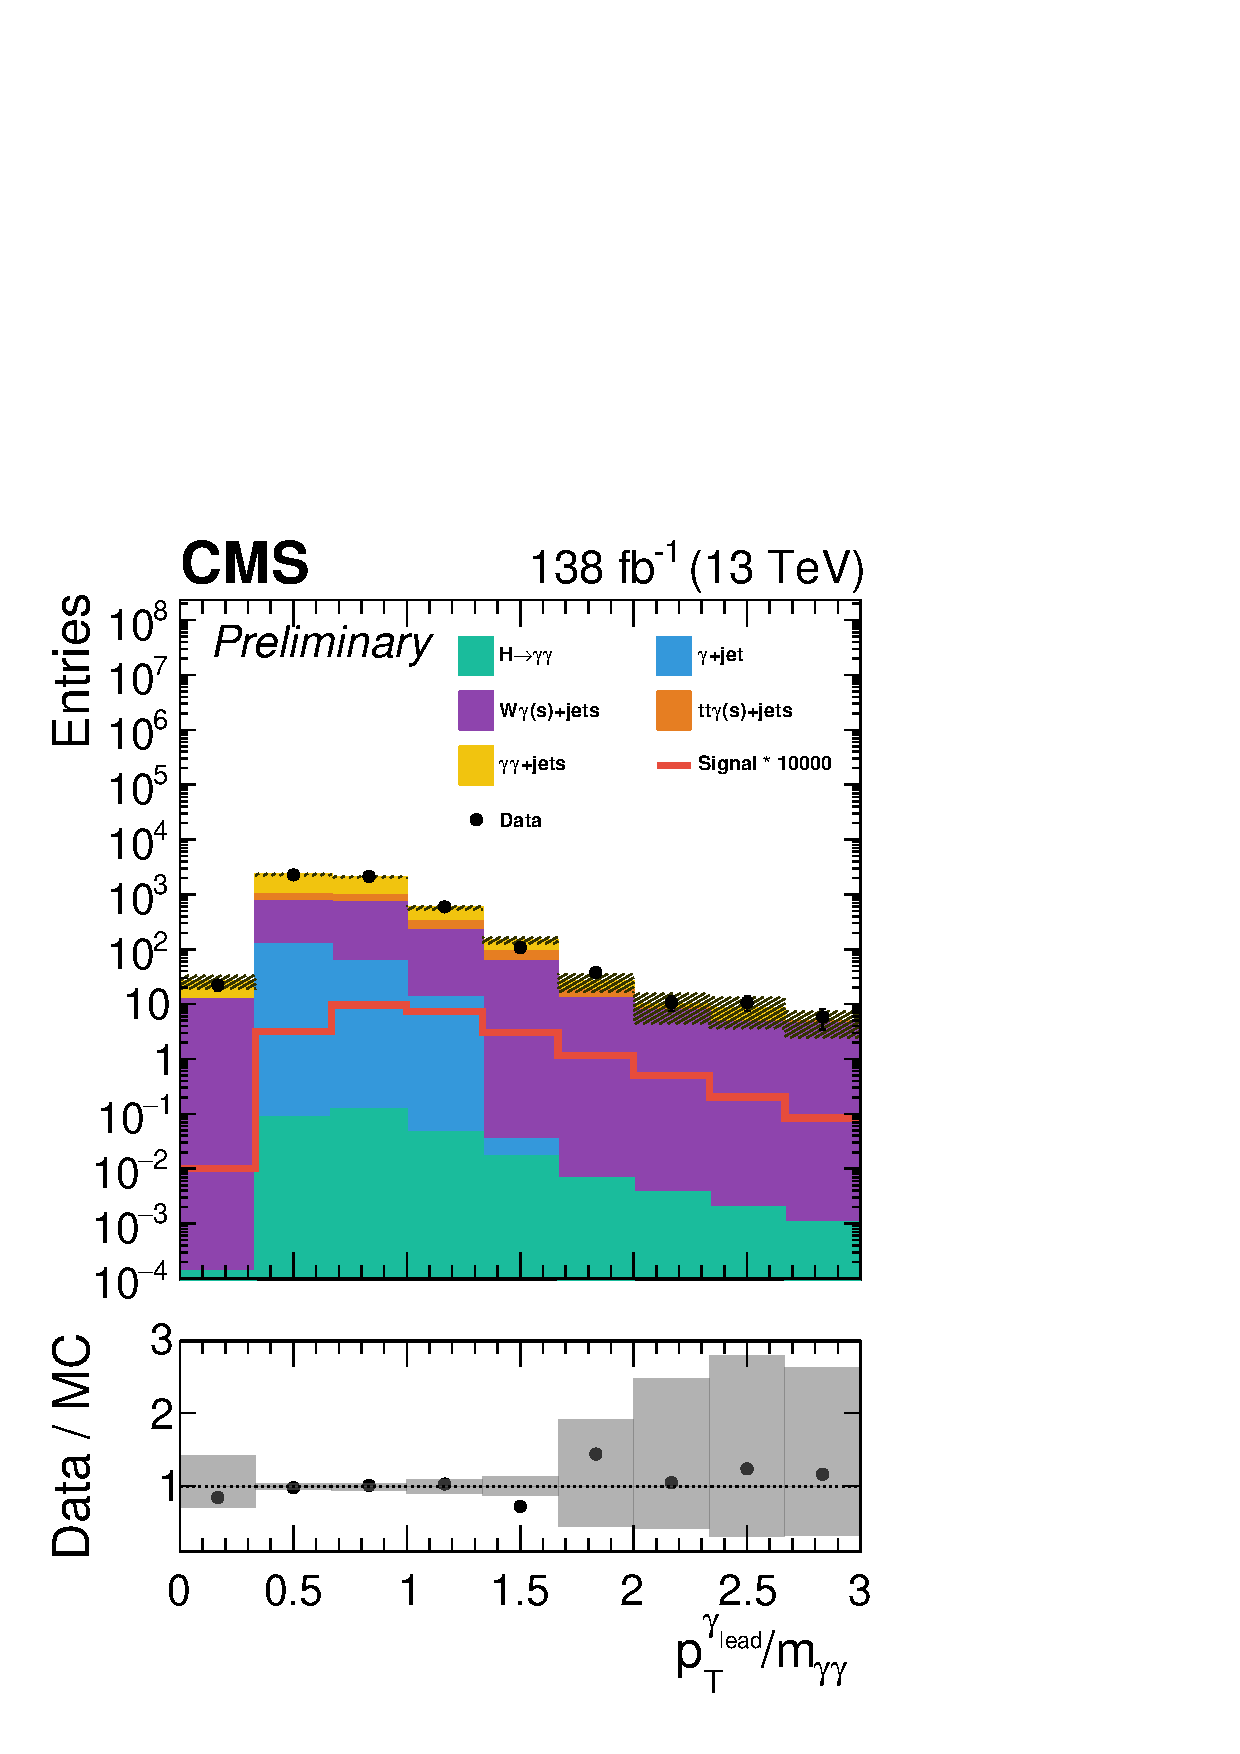
\includegraphics[width=0.47\textwidth]{Sections/HHWWgg/images/DNN/DataMC/DataMC_Scaled_Leading_Photon_pt_FullRegion_log.pdf}}
\subfloat[Scaled Subleading Photon \pt]{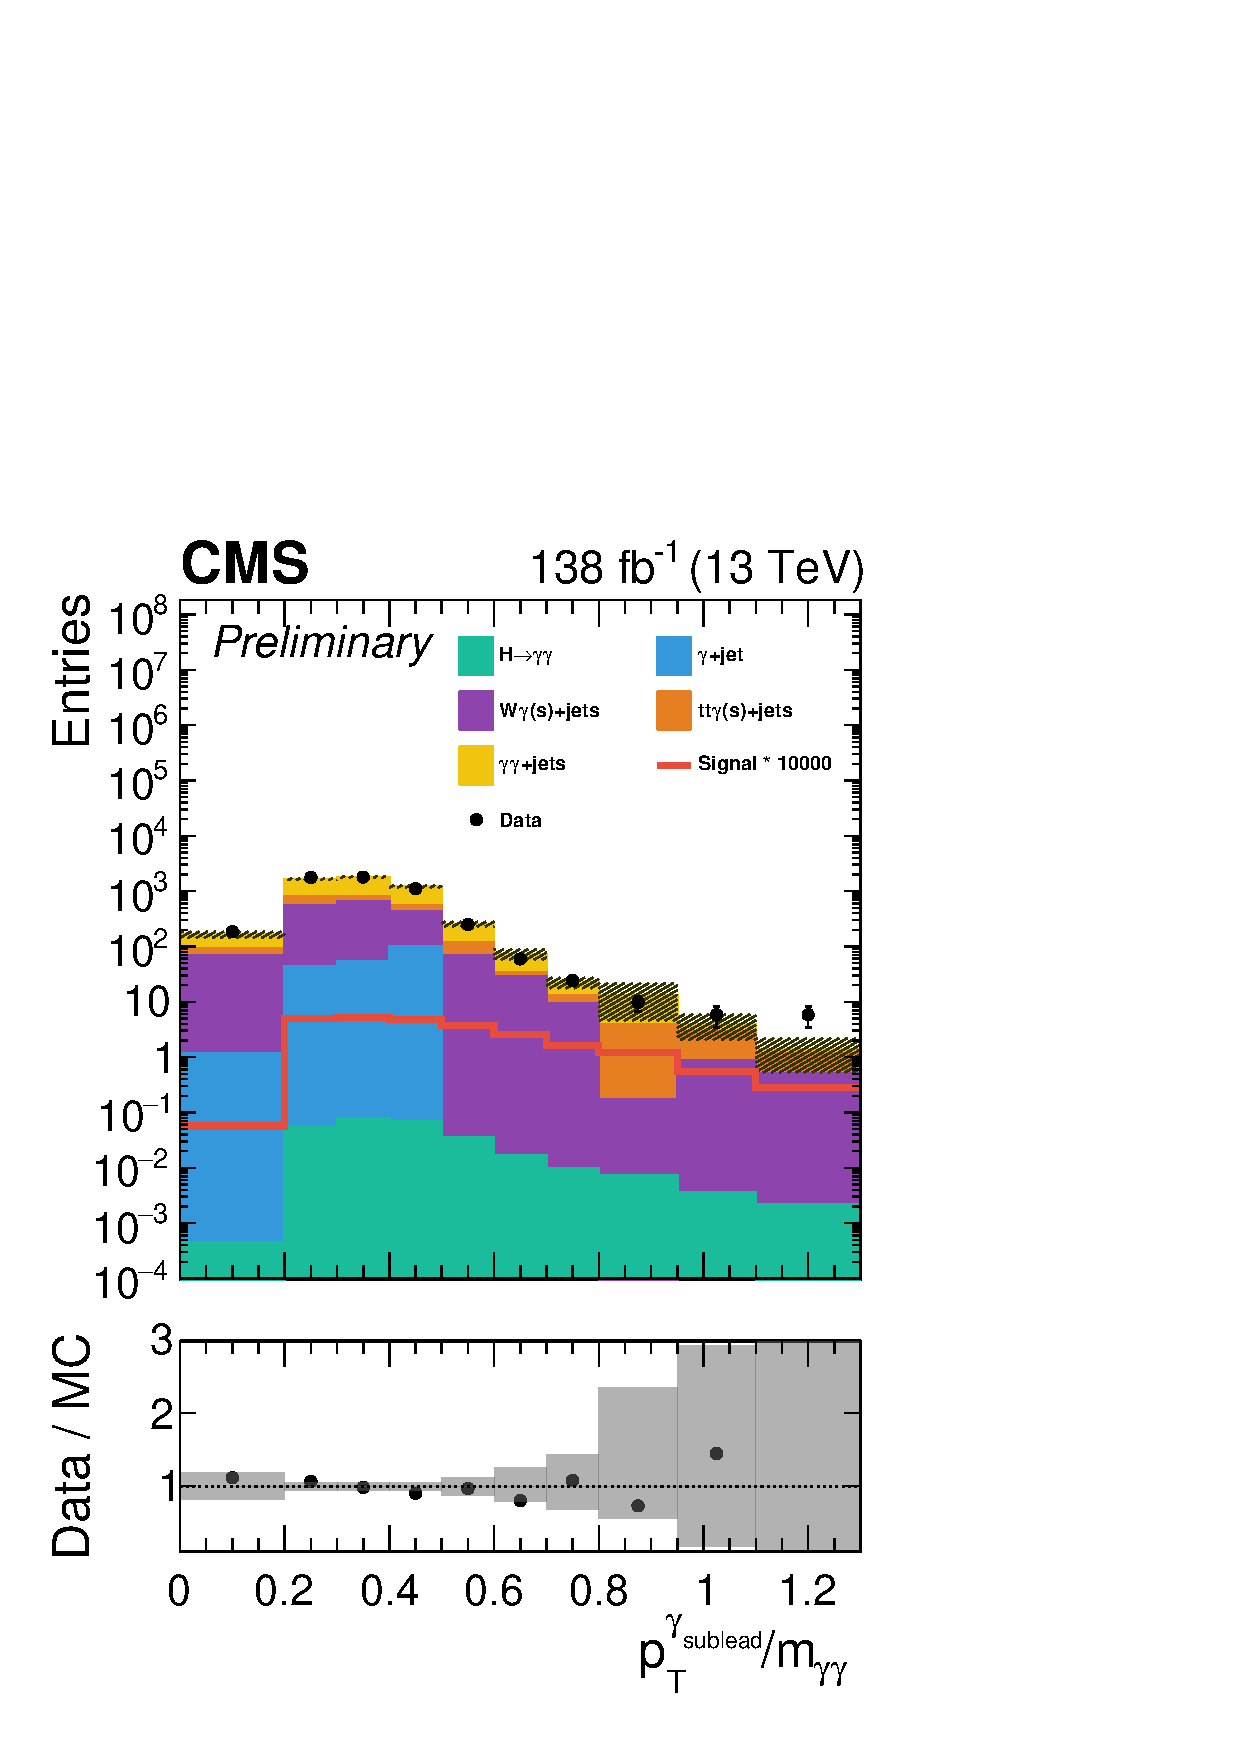
\includegraphics[width=0.47\textwidth]{Sections/HHWWgg/images/DNN/DataMC/DataMC_Scaled_Subleading_Photon_pt_FullRegion_log.pdf}}
\caption{Data/MC ratio of semi-leptonic channel input features in full mass region}
\label{fig:SLDNNFeaturecontrolplots-1}
\end{figure}

\begin{figure}[H]
  \setcounter{subfigure}{0}
  \centering
  \subfloat[Lepton energy]{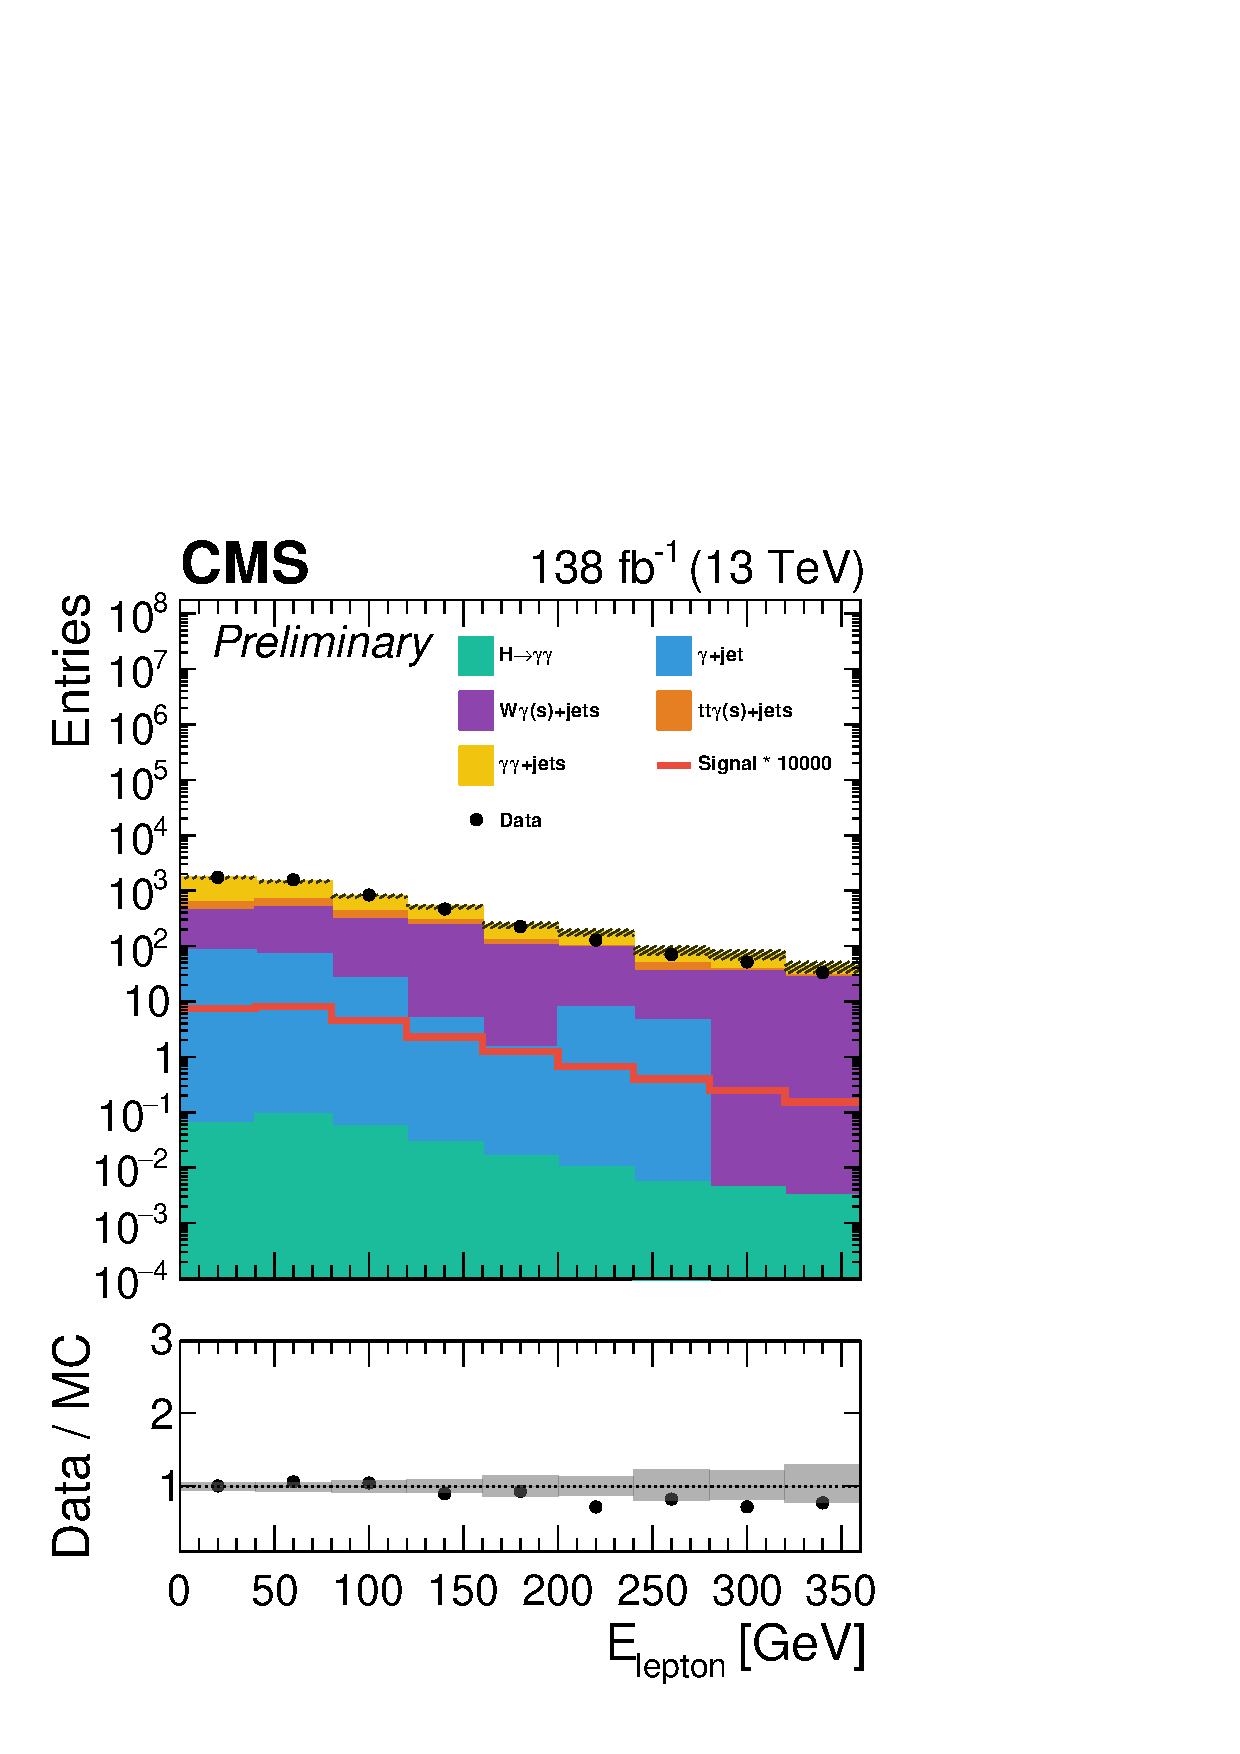
\includegraphics[width=0.47\textwidth]{Sections/HHWWgg/images/DNN/DataMC/DataMC_goodLepton_E_FullRegion_log.pdf}}
  \subfloat[Leading jet \pt \label{fig:lead_jet_pt}]{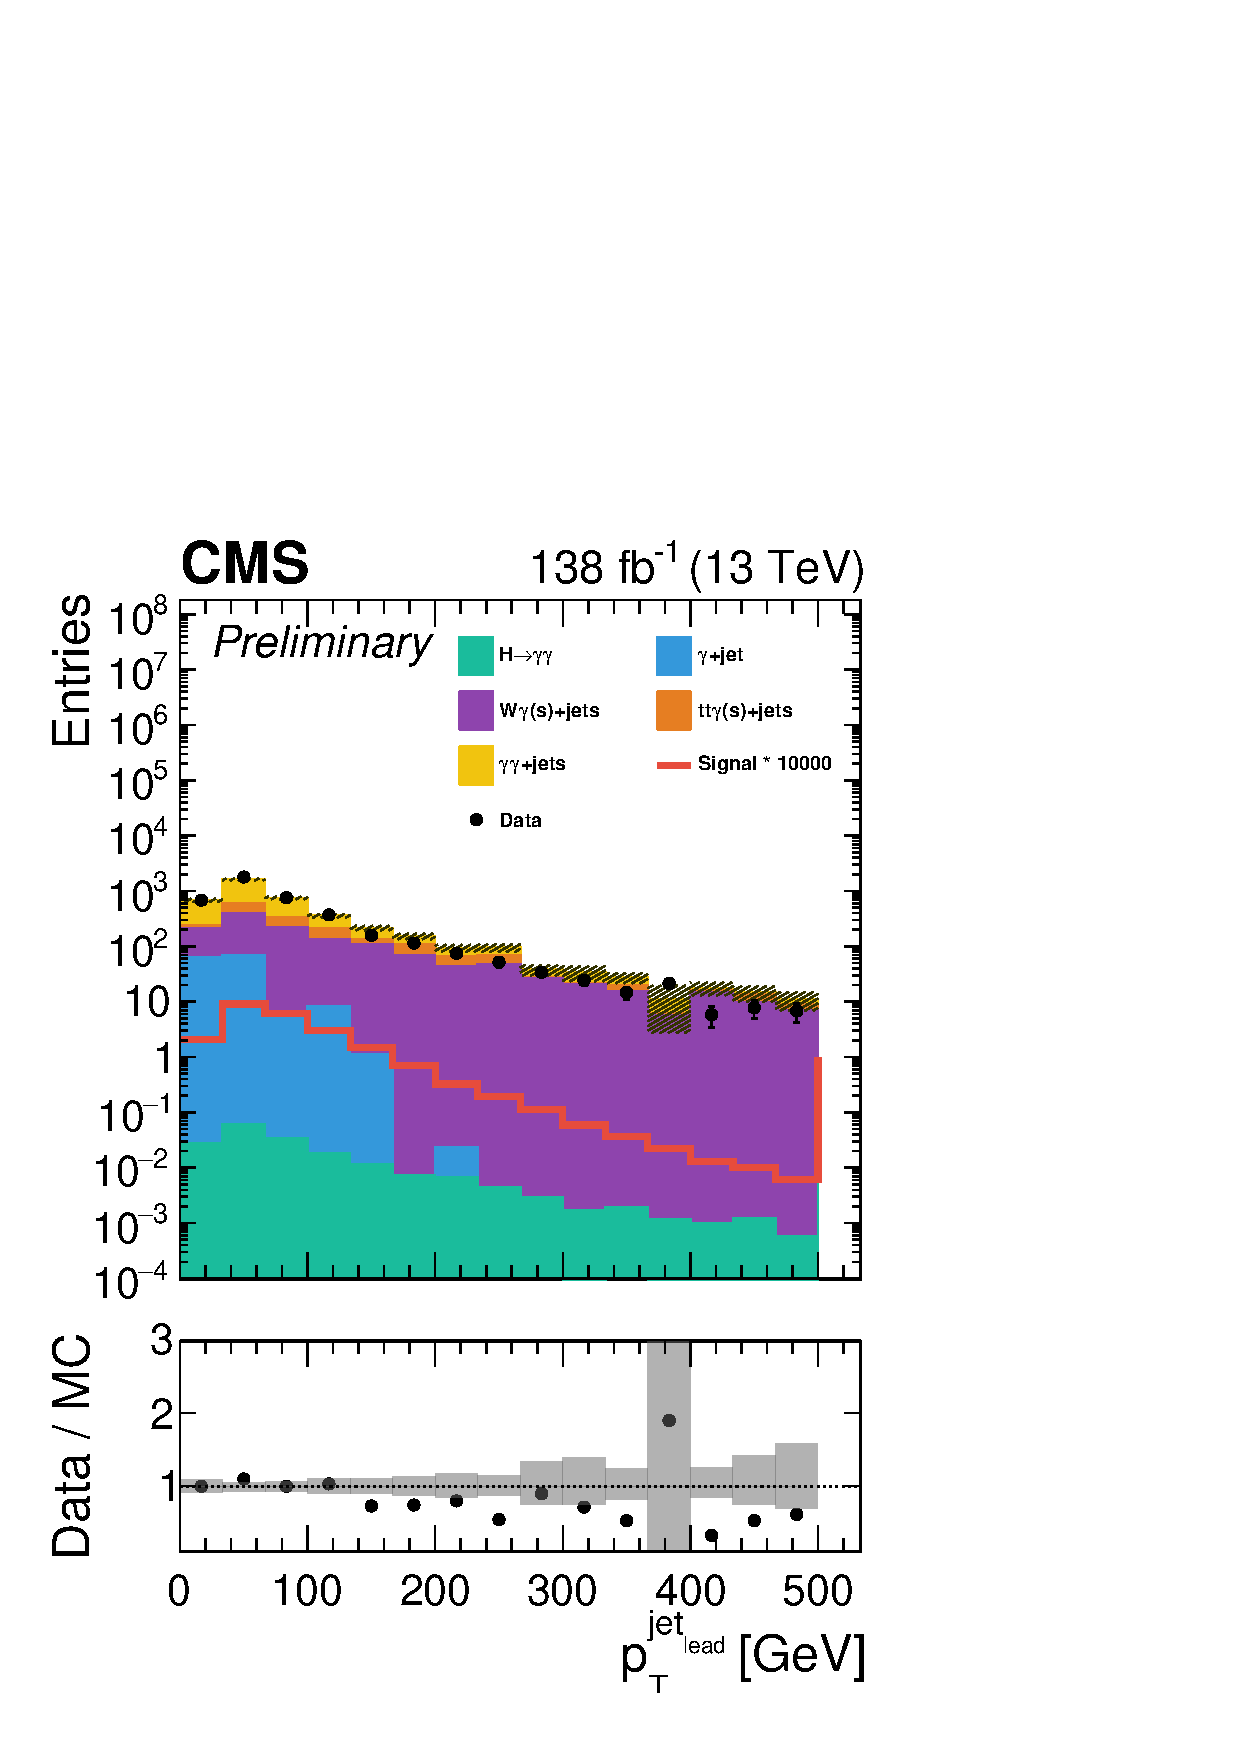
\includegraphics[width=0.47\textwidth]{Sections/HHWWgg/images/DNN/DataMC/DataMC_goodJets_0_pt_FullRegion_log.pdf}}
  \caption{Data/MC ratio of semi-leptonic channel input features in full mass region}
  \label{fig:SLDNNFeaturecontrolplots-2}
\end{figure}

\begin{table}[H]
  \begin{center}
          \begin{tabular}{c|c|c}
                  MC Sample & Unweighted & Weighted \\ \hline
                  DiPhoJetsBox\_MGG-80toInf & 5108 & 581.97343 \\
                  GJet\_40toInf & 110 & 48.26491 \\
                  tt$\gamma\gamma+$0Jets & 4633 & 17.01703 \\
                  tt$\gamma+$Jets & 1564 & 52.52178 \\
                  tt$+$Jets & 288 & 51.77128 \\
                  W1Jets\_pT\_150-250 & 1298 & 64.88303 \\
                  W1Jets\_pT\_250-400 & 341 & 7.42416 \\
                  W1Jets\_pT\_400-inf & 217 & 1.80622 \\
                  W1Jets\_pT\_50-150 & 23 & 13.60197 \\
                  W2Jets\_pT\_150-250 & 1612 & 60.29933 \\
                  W2Jets\_pT\_250-400 & 777 & 12.25016 \\
                  W2Jets\_pT\_400-inf & 531 & 3.05085 \\
                  W2Jets\_pT\_50-150 & 59 & 27.52279 \\
                  WGGJets & 360 & 132.12192 \\
                  WGJJToLNu\_EWK\_QCD & 140 & 30.91906 \\
                  ttWJets & 74 & 0.5721 \\ \hline                
          \end{tabular}
  \captionof{table}{Unweighted and weighted training MC yields in the \mgg sideband region, including semi-leptonic training pre-selections and only events with a DNN output score $>$ 0.1. \label{tab:SL_DNN_Background_yields}}
  \end{center}
\end{table}


\begin{figure}
\caption{Pairwise Spearman's correlation (monotonic relationships) between semileptonic channel DNN input features.}
\setlength{\unitlength}{1mm}
\begin{center}
\mbox{
\includegraphics*[height=150mm]{Sections/HHWWgg/images/DNN/correlation_plot.pdf}
  }
\end{center}
\label{fig:inputvarcorrelation}
\end{figure}

% \begin{figure}[H]
%   \setcounter{subfigure}{0}
%   \centering
%   \subfloat[All Shapley scores]{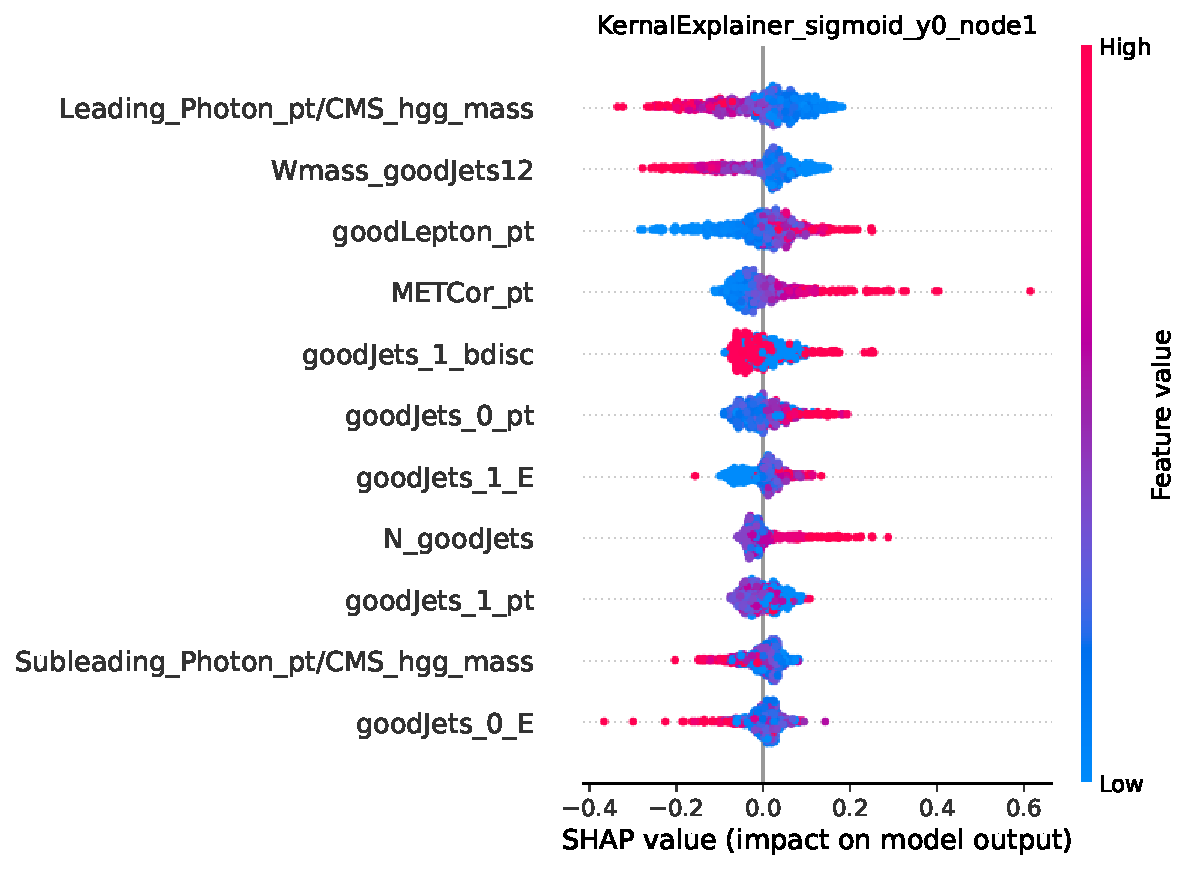
\includegraphics[width=0.45\textwidth]{Sections/HHWWgg/images/DNN/KernalExplainer_sigmoid_y0_node1.pdf}}
%   %\qquad
%   \subfloat[Average Shapley score magnitudes]{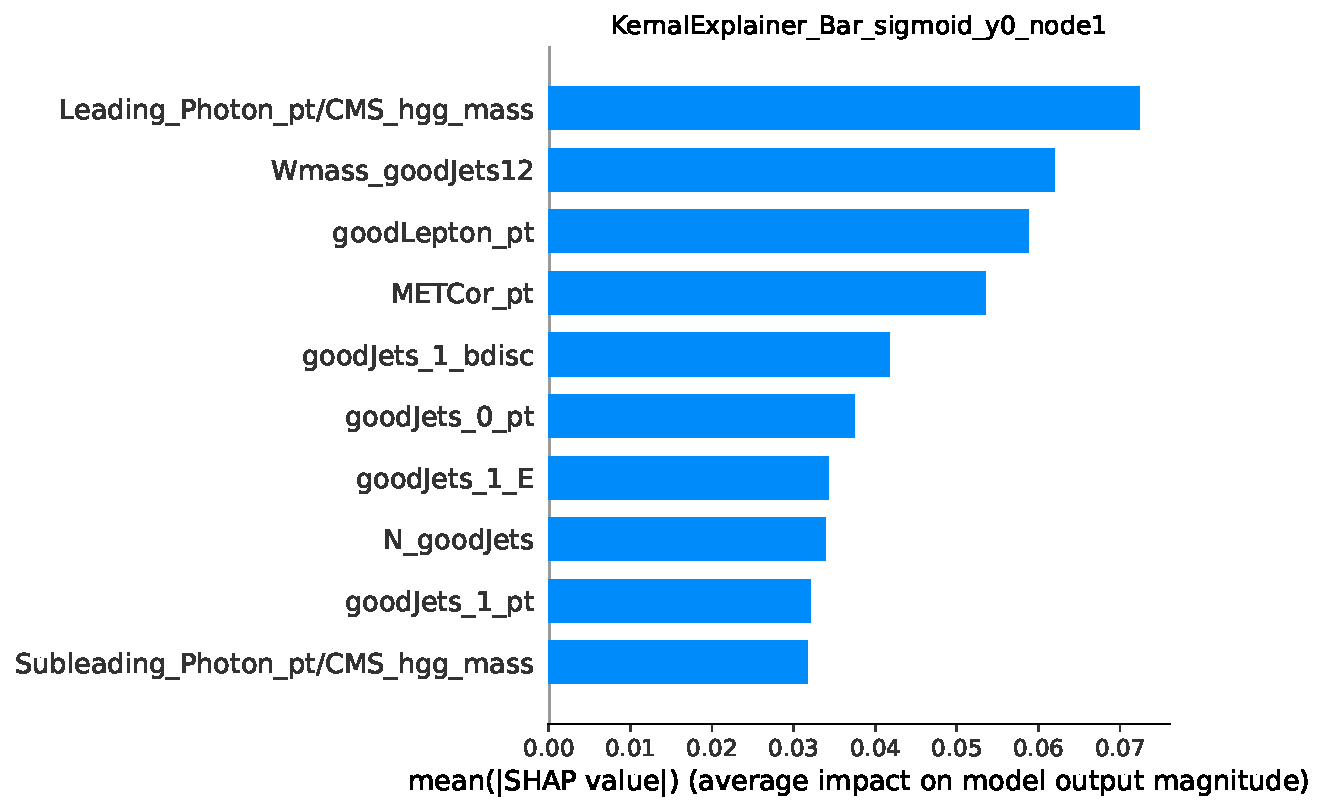
\includegraphics[width=0.45\textwidth]{Sections/HHWWgg/images/DNN/KernalExplainer_Bar_sigmoid_y0_node1.pdf}}
%   \caption{Semi-leptonic channel DNN input feature ranking according to Shapely values in the H class}
%   \label{fig:SLfeatureranking_H}
% \end{figure} 

% \begin{figure}[H]
%   \setcounter{subfigure}{0}
%   \centering
%   \subfloat[All Shapley scores]{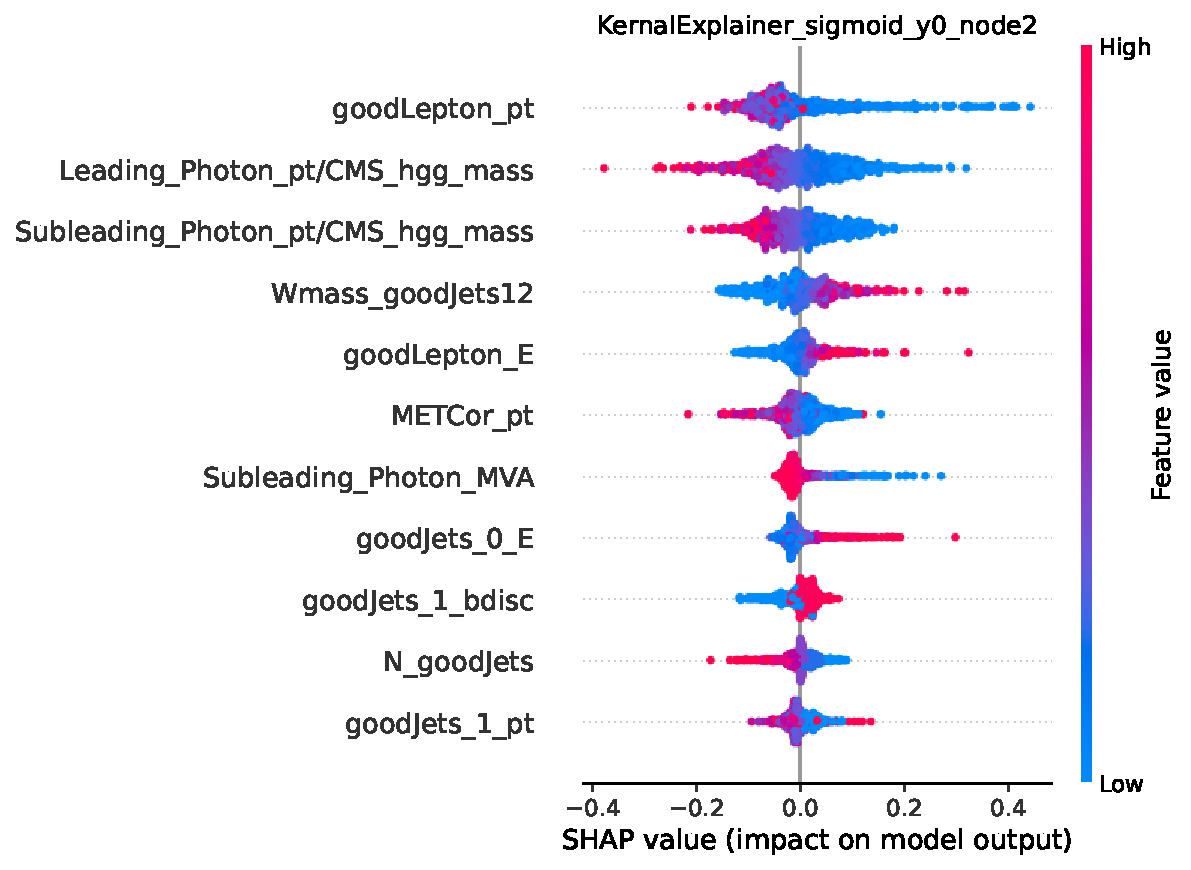
\includegraphics[width=0.45\textwidth]{Sections/HHWWgg/images/DNN/KernalExplainer_sigmoid_y0_node2.pdf}}
%   %\qquad
%   \subfloat[Average Shapley score magnitudes]{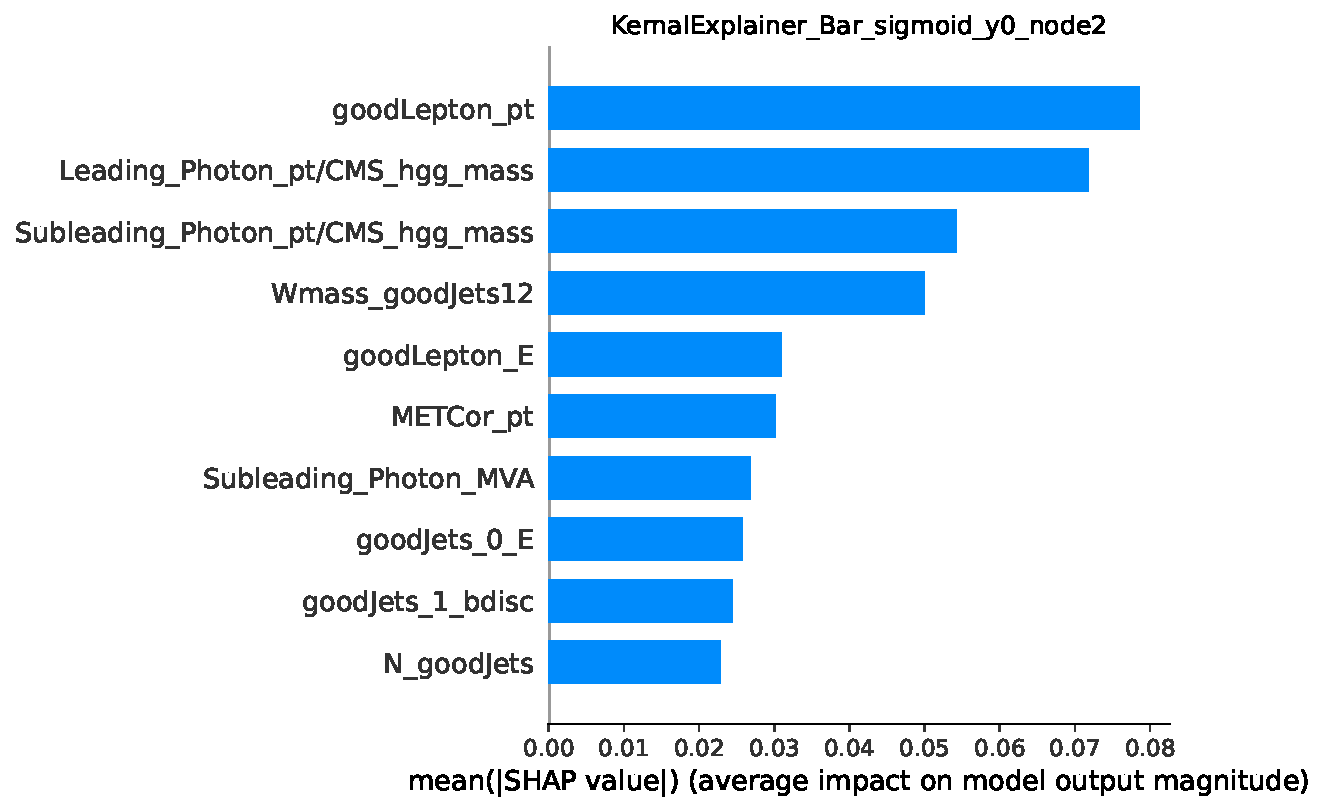
\includegraphics[width=0.45\textwidth]{Sections/HHWWgg/images/DNN/KernalExplainer_Bar_sigmoid_y0_node2.pdf}}
%   \caption{Semi-leptonic channel DNN input feature ranking according to Shapely values in the Continuum background class}
%   \label{fig:SLfeatureranking_bkg}
% \end{figure} 

% The network hyper-parameter settings for the trained semi-leptonic channel DNN can be found in table \ref{tab:hypparams} and the architecture can be found
% in figure \ref{fig:DNNarch}. Several architectures were investigated in an attempt to give the model enough flexibility to model decision boundaries in high-dimensionality 
% phase-space, while ensuring the model is trainable with the size of our dataset. Once the networks architecture was established, a hyper-parameter scan was performed on the number of epochs, learning rate and batch size. 
% The optimal network performance was achieved with the chosen parameters. The performance of networks of a given architecture was found to be relatively robust to further
% fine-tuning of hyper-parameters.

% The output ROC curves from training for each class can be seen in Figures \ref{fig:ROC_HH}, \ref{fig:ROC_H} and \ref{fig:ROC_bkg}, shown together for all 
% training and test sets in Figure \ref{fig:All_ROCs}. The corresponding
% loss vs. epoch trend is shown in Figure \ref{fig:LossVsEpoch} for a test and training set of data, where 90\% of sample events are reserved for training and the other 10\% for the test dataset 
% in order to check for overtraining. Additionally, the normalized HH, H, and Continuum background DNN output scores are plotted for training and test samples to check for overtraining, as shown in Figures \ref{fig:SL_DNN_overfitting_check}, 
% \ref{fig:SL_DNN_overfitting_check_SingleH} and \ref{fig:SL_DNN_overfitting_check_ContBkg}. For 
% all three types of events, HH, H and continuum background, the distributions of the HH, H and continuum background node DNN scores for training and test samples are in agreement, a further indication that there is no overtraining and therefore 
% no loss in sensitivity due to overtraining.

The output DNN score comparison between the data
and MC is shown in Figure \ref{fig:SL_DNN_Score}. In this comparison, events with a DNN score less than 0.1 are removed as they are not used in categorization or signal modeling.

Finally, the output DNN score for data events in the sidebands and signal events in the signal region are shown in Figure \ref{fig:YearByYear_DNN_Scores}, not including 
events with a DNN score less than 0.1 as they are not used in the analysis. Each signal histogram is normalized to an integral of 1, and each data histogram is normalized to the luminosity of the 2018 dataset.
It can be seen that the shapes are very similar per year, and that there is no clear systematic difference when applying the 2017-only trained DNN on 
2016 and 2018 data and signal events. The data histograms are shown in log scale in order to highlight that there are similar DNN score shapes per year which appear similar within statistical uncertainty,
in particular in the high DNN score region which is the most signal sensitive region. 

% \begin{figure}[H]
%   \caption{Semi-Leptonic DNN ROC curve for training and test data: H Class}
%   \setlength{\unitlength}{1mm}
%   \begin{center}
%     \mbox{\includegraphics*[height=100mm]{Sections/HHWWgg/images/DNN/MultiClass_ROC_class_H.pdf}
%     }
%   \end{center}
%   \label{fig:ROC_H}
% \end{figure}

% \begin{figure}[H]
%   \caption{Semi-Leptonic DNN ROC curve for training and test data: Continuum Background class}
%   \setlength{\unitlength}{1mm}
%   \begin{center}
%     \mbox{\includegraphics*[height=100mm]{Sections/HHWWgg/images/DNN/MultiClass_ROC_class_Bkg.pdf}
%     }
%   \end{center}
%   \label{fig:ROC_bkg}
% \end{figure}

% \begin{figure}[H]
%   \setcounter{subfigure}{0}
%   \centering
%   \subfloat[Test samples]{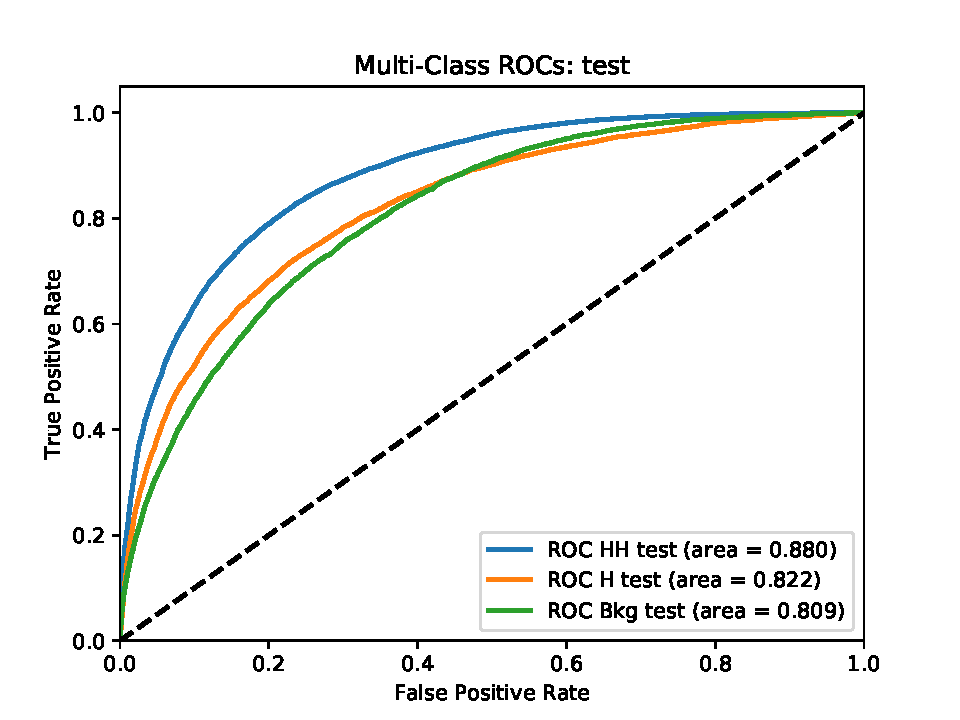
\includegraphics[width=0.45\textwidth]{Sections/HHWWgg/images/DNN/MultiClass_ROC_dataset_test.pdf}}
%   \qquad
%   \subfloat[Training samples]{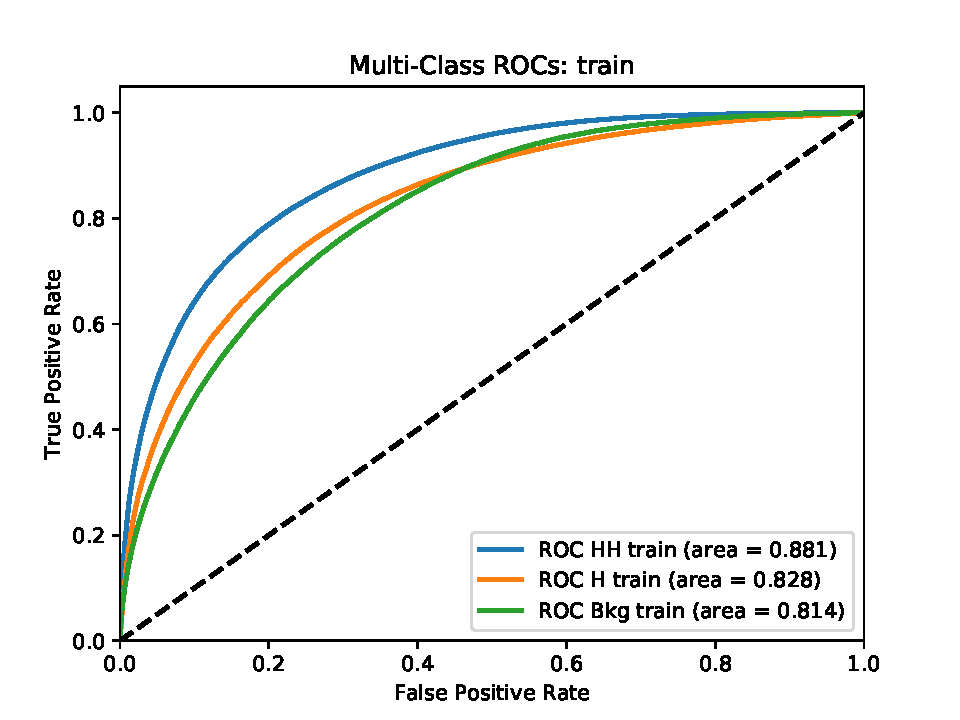
\includegraphics[width=0.45\textwidth]{Sections/HHWWgg/images/DNN/MultiClass_ROC_dataset_train.pdf}}
%   \caption{ROC curves of three MultiClass nodes}
%   \label{fig:All_ROCs}
% \end{figure} 

% \begin{figure}[H]
%   \caption{Semi-Leptonic DNN loss vs. epoch for training and test data}
%   \setlength{\unitlength}{1mm}
%   \begin{center}
%     \mbox{\includegraphics*[height=100mm]{Sections/HHWWgg/images/DNN/history_loss.pdf}
    
%     }
%   \end{center}
%   \label{fig:LossVsEpoch}
% \end{figure}

% \begin{figure}[H]
%   \setlength{\unitlength}{1mm}
%   \begin{center}
%     \mbox{\includegraphics*[height=100mm]{Sections/HHWWgg/images/DNN/overfitting_plot_Single_H_Non-Categorised.pdf}
%     }
%   \end{center}
%   \caption{Normalized Single Higgs DNN score distributions for the three semileptonic DNN nodes, shown for training and test events.}
%   \label{fig:SL_DNN_overfitting_check_SingleH}
% \end{figure}

% \begin{figure}[H]
%   \setlength{\unitlength}{1mm}
%   \begin{center}
%     \mbox{\includegraphics*[height=100mm]{Sections/HHWWgg/images/DNN/overfitting_plot_Cont_Bkg_Non-Categorised.pdf}
%     }
%   \end{center}
%   \caption{Normalized Continuum Background DNN score distributions for the three semileptonic DNN nodes, shown for training and test events.}
%   \label{fig:SL_DNN_overfitting_check_ContBkg}
% \end{figure}


% \begin{table}[H]
%     \begin{center}
%   \caption{Hyper-parameter settings for semi-leptonic channel DNN}
%   \resizebox{100mm}{!}{
%   \begin{tabular}{| l | l |}
%     \hline
%     Hyper-parameter & Setting \\
%     \hline
%     Epochs & 500 \\
%     Batch size &  500 \\
%     Learning rate & 0.0001 \\
%     Optimiser & Nadam \\
%     Loss function & categorical$\_$crossentropy \\
%     Kernel initialiser & glorot normal \\
%     Hidden layer activation functions & ReLU \\
%     Output layer activation function & softmax \\
%     \hline
%   \end{tabular}
%   }
%   \label{tab:hypparams}
%   \end{center}
% \end{table}

% \begin{figure}
%     \caption{Schematic of semi-leptonic DNN model architecture. The sequential DNN model shows the various layer names along with the dimensions of the input and output vectors. One can see that a vector of 29 input variables is condensed down into a binary output value in the last layer.}
%   \setlength{\unitlength}{1mm}
%   \begin{center}
%     \mbox{\includegraphics*[height=150mm]{Sections/HHWWgg/images/DNN/model_schematic.pdf}
%     }
%   \end{center}
%   \label{fig:DNNarch}
% \end{figure}

% \begin{figure}[H]
%   \setcounter{subfigure}{0}
%   \centering
%   \subfloat[Linear y scale]{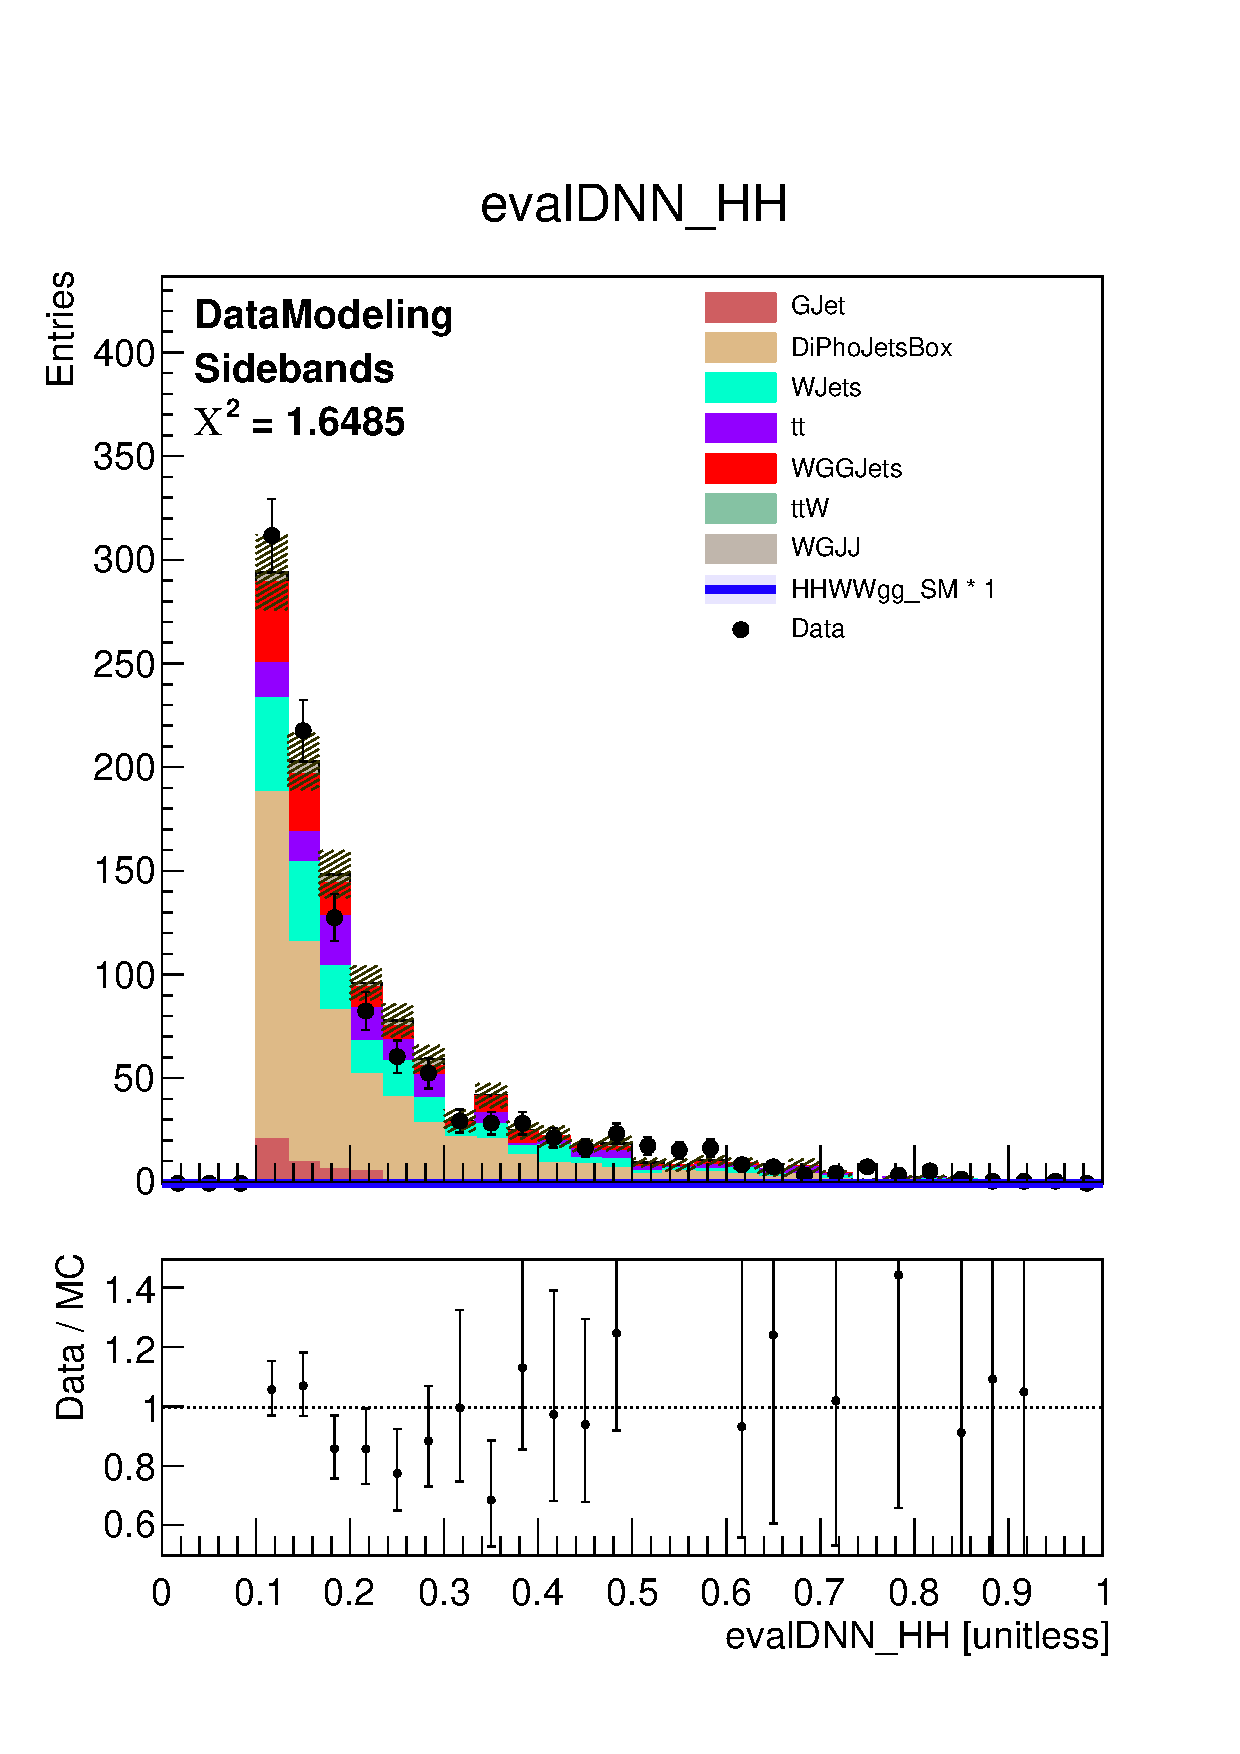
\includegraphics[width=0.45\textwidth]{Sections/HHWWgg/images/DNN/DataMC/DataMC_evalDNN_HH_SB_nonLog.pdf}}
%   \qquad
%   \subfloat[Logarithmic y scale]{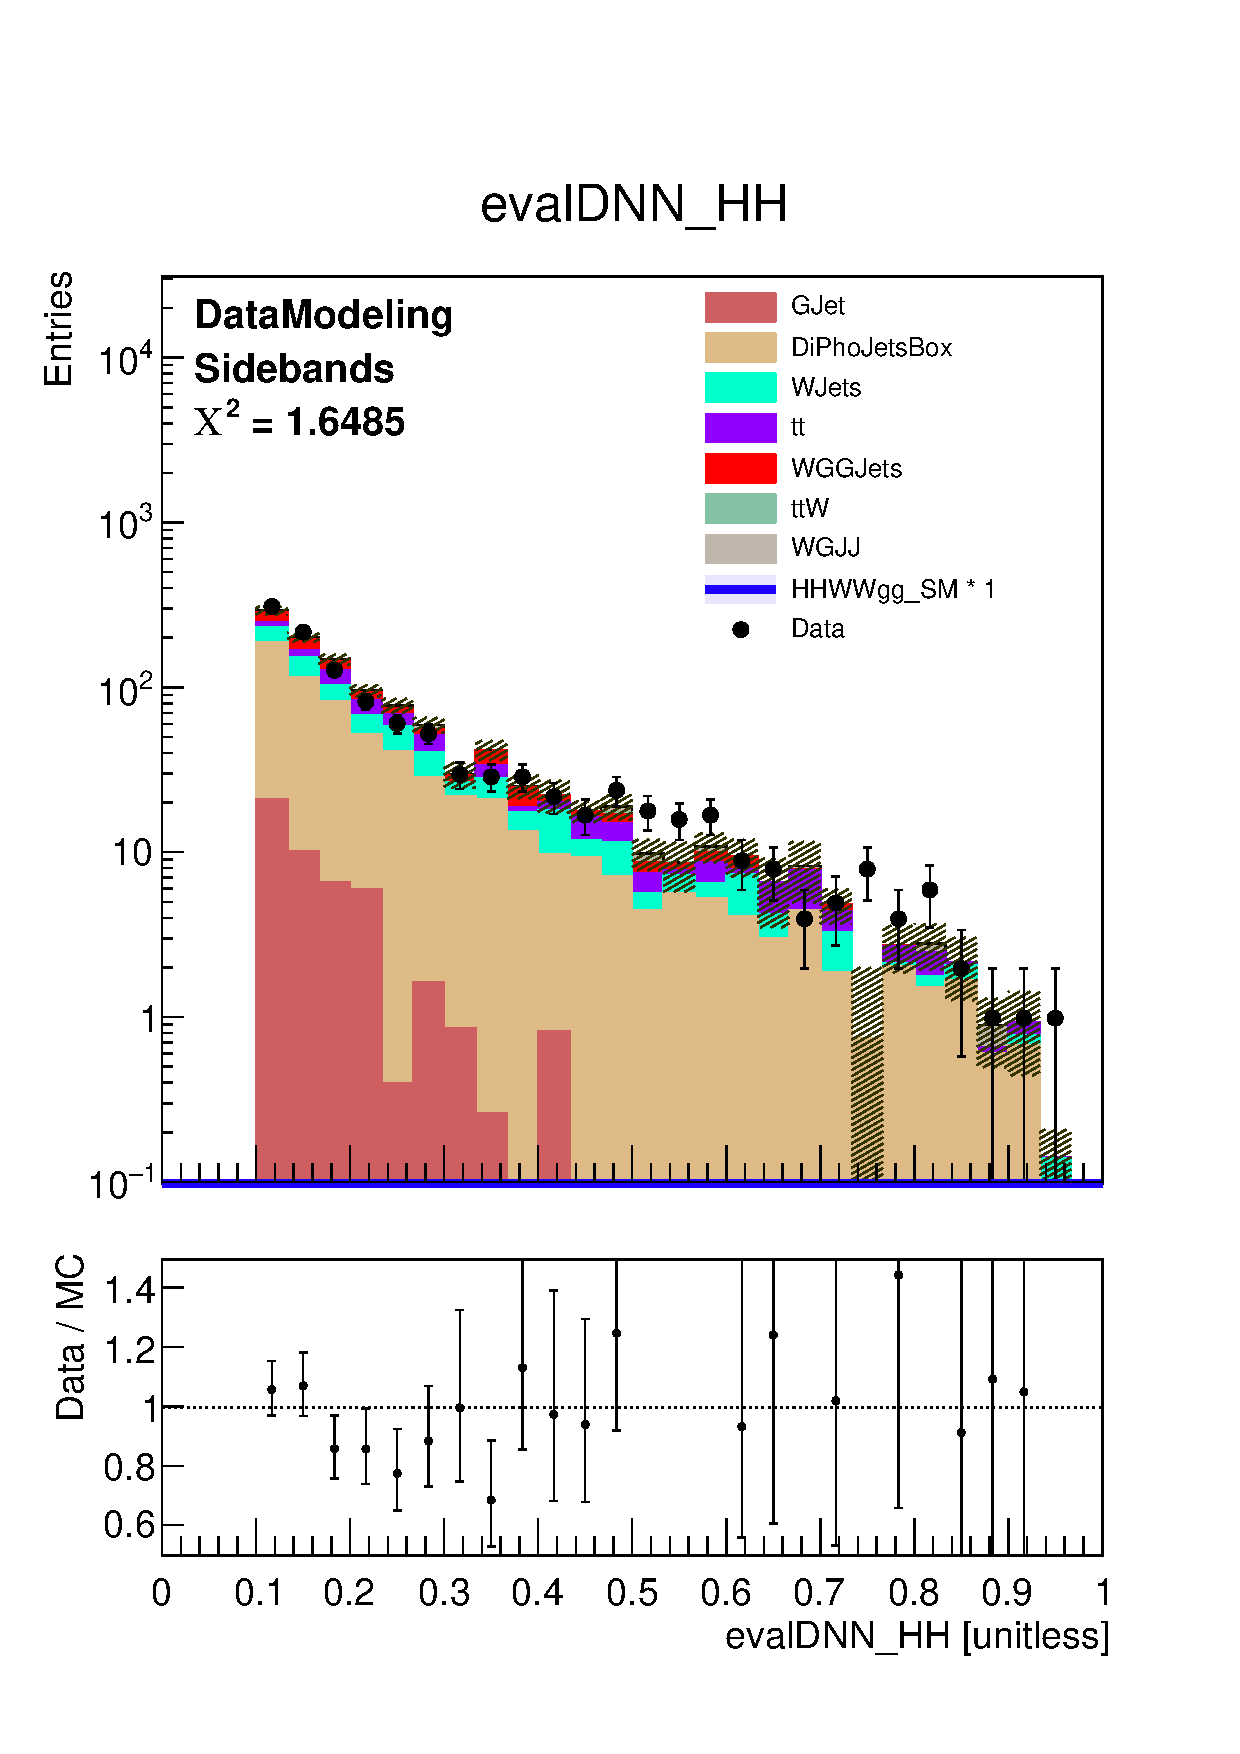
\includegraphics[width=0.45\textwidth]{Sections/HHWWgg/images/DNN/DataMC/DataMC_evalDNN_HH_SB_log.pdf}}
%   \caption{Output DNN score for 2017 data and MC in the signal sideband. A logarithmic y scale version is included in order to see the low statistics bins.}
%   \label{fig:DNNscore_Data_MC}
% \end{figure} 

\begin{figure}[H]
    \centering
    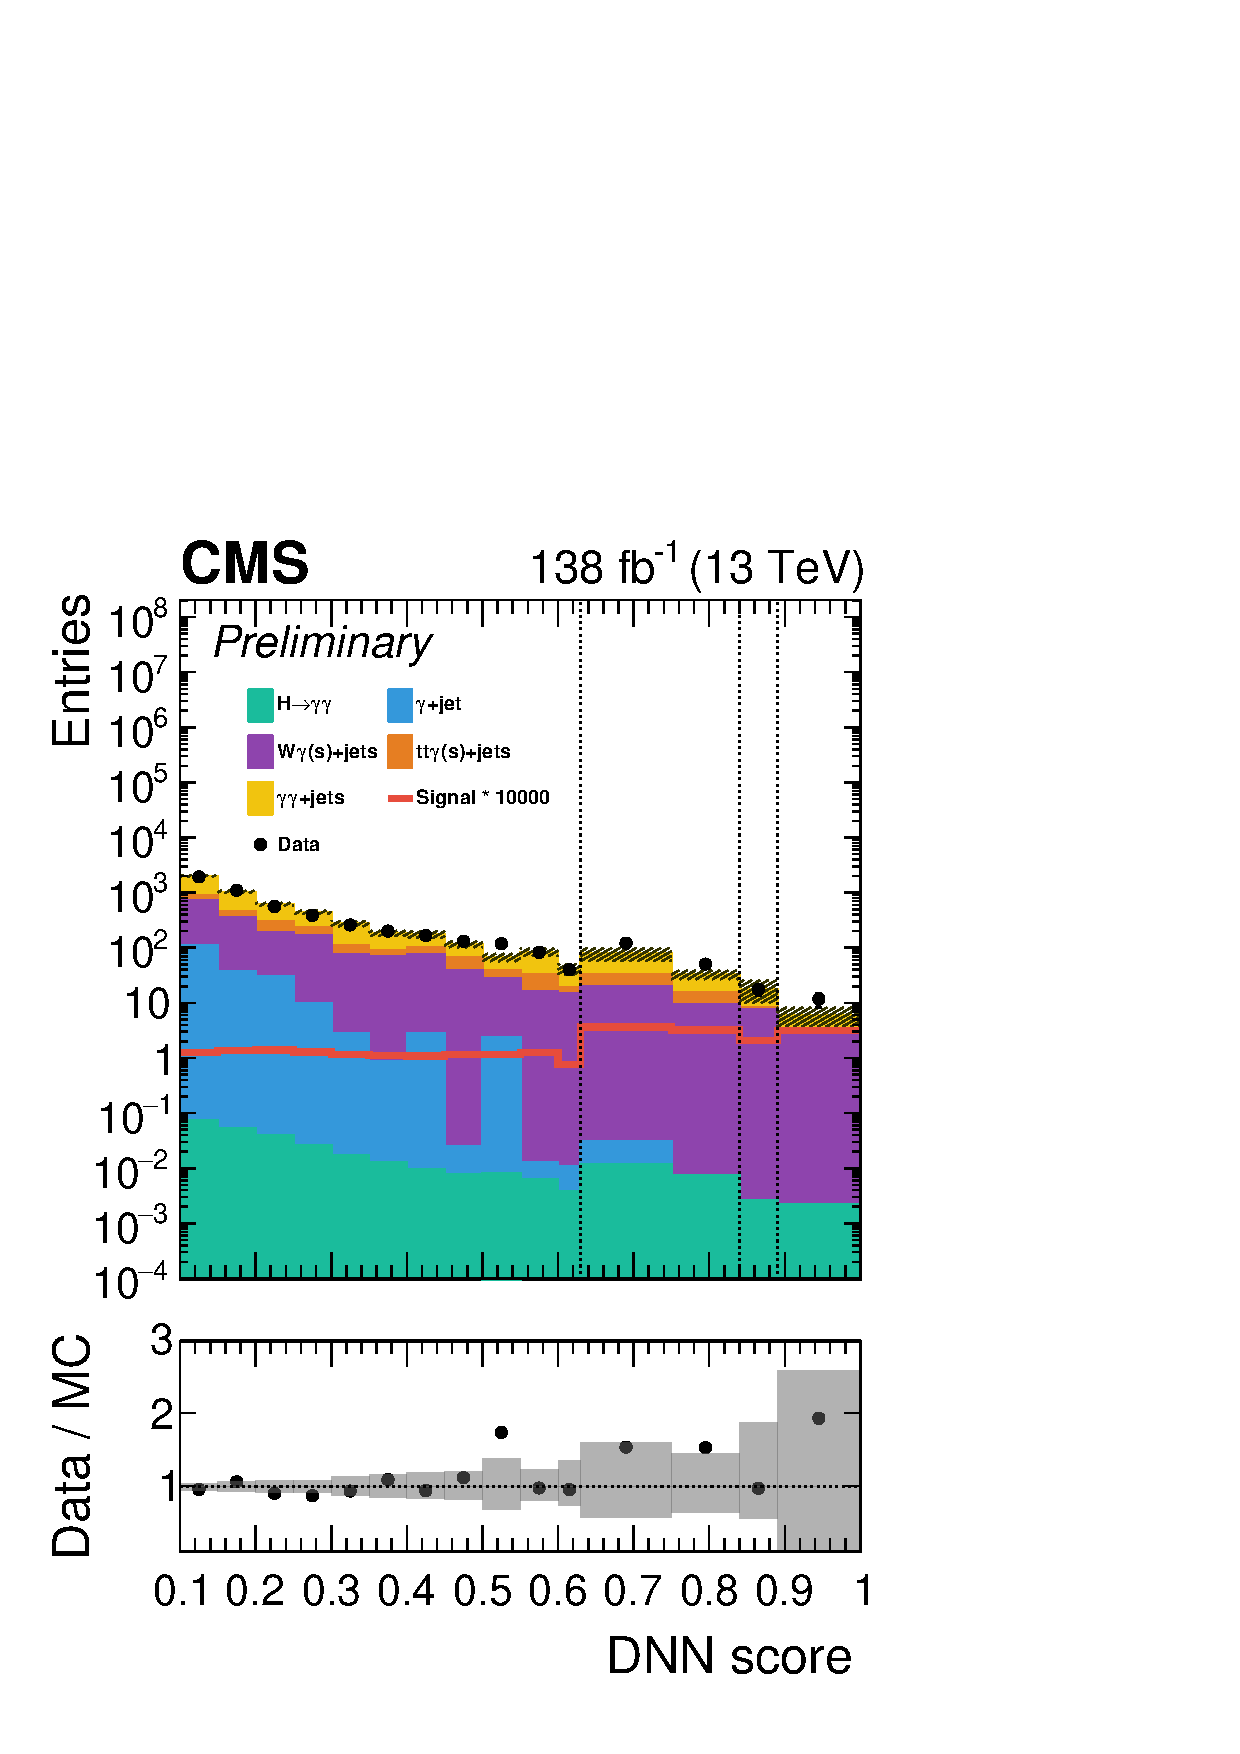
\includegraphics[width=\textwidth]{Sections/HHWWgg/images/DNN/DataMC/DataMC_evalDNN_HH_FullRegion_log.pdf}
    \caption{DNN output score between data and MC, using Run 2 dataset and 2017 MC scaled to Run 2 lumi.}
    \label{fig:SL_DNN_Score}
\end{figure}

\begin{figure}[H]
  \setcounter{subfigure}{0}
  \centering
  \subfloat[Data in data sideband, each year scaled to 2018 luminosity]{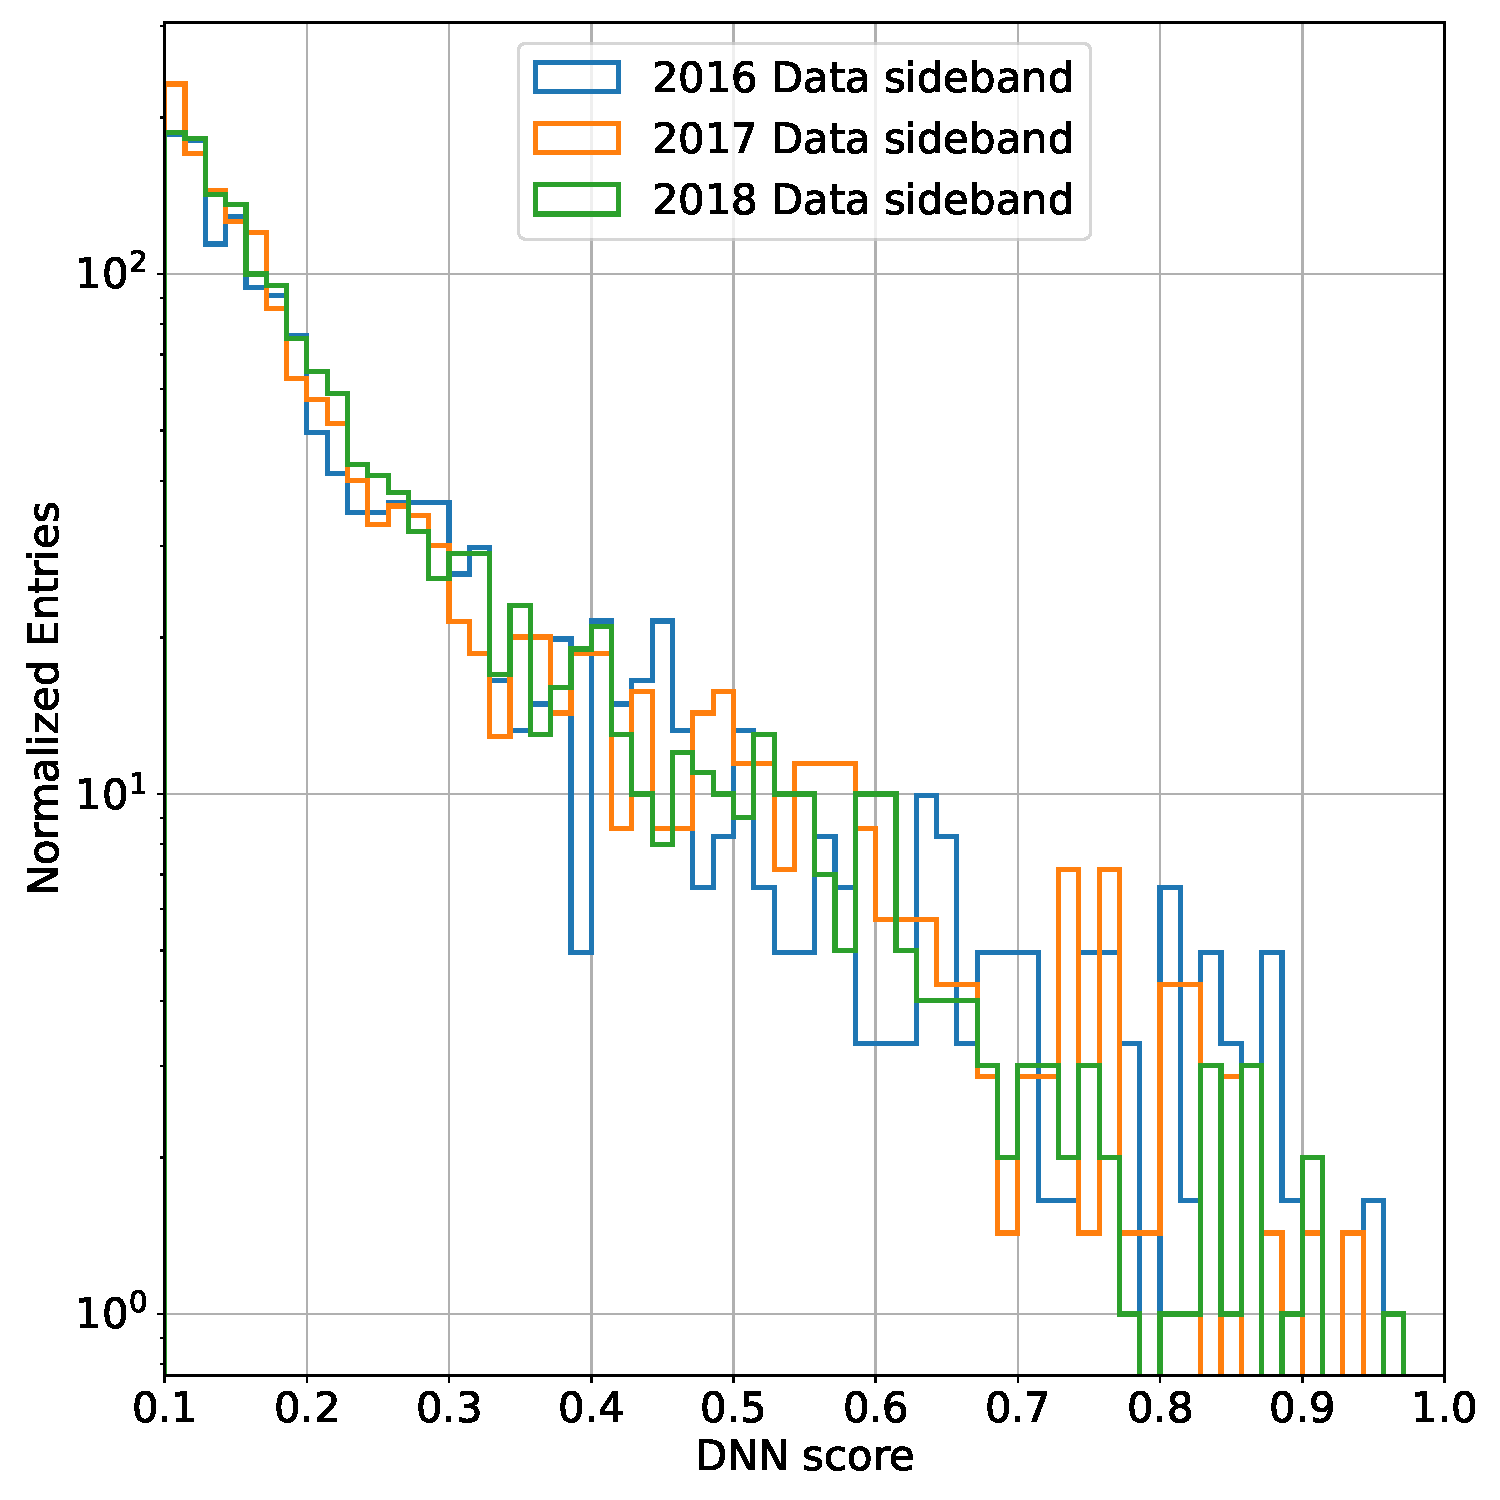
\includegraphics[width=0.45\textwidth]{Sections/HHWWgg/images/DNN/YearByYear_SLDNN_scores_Data_log.pdf}}
  \qquad
  \subfloat[Signal in signal region, each histogram normalized to an integral of 1]{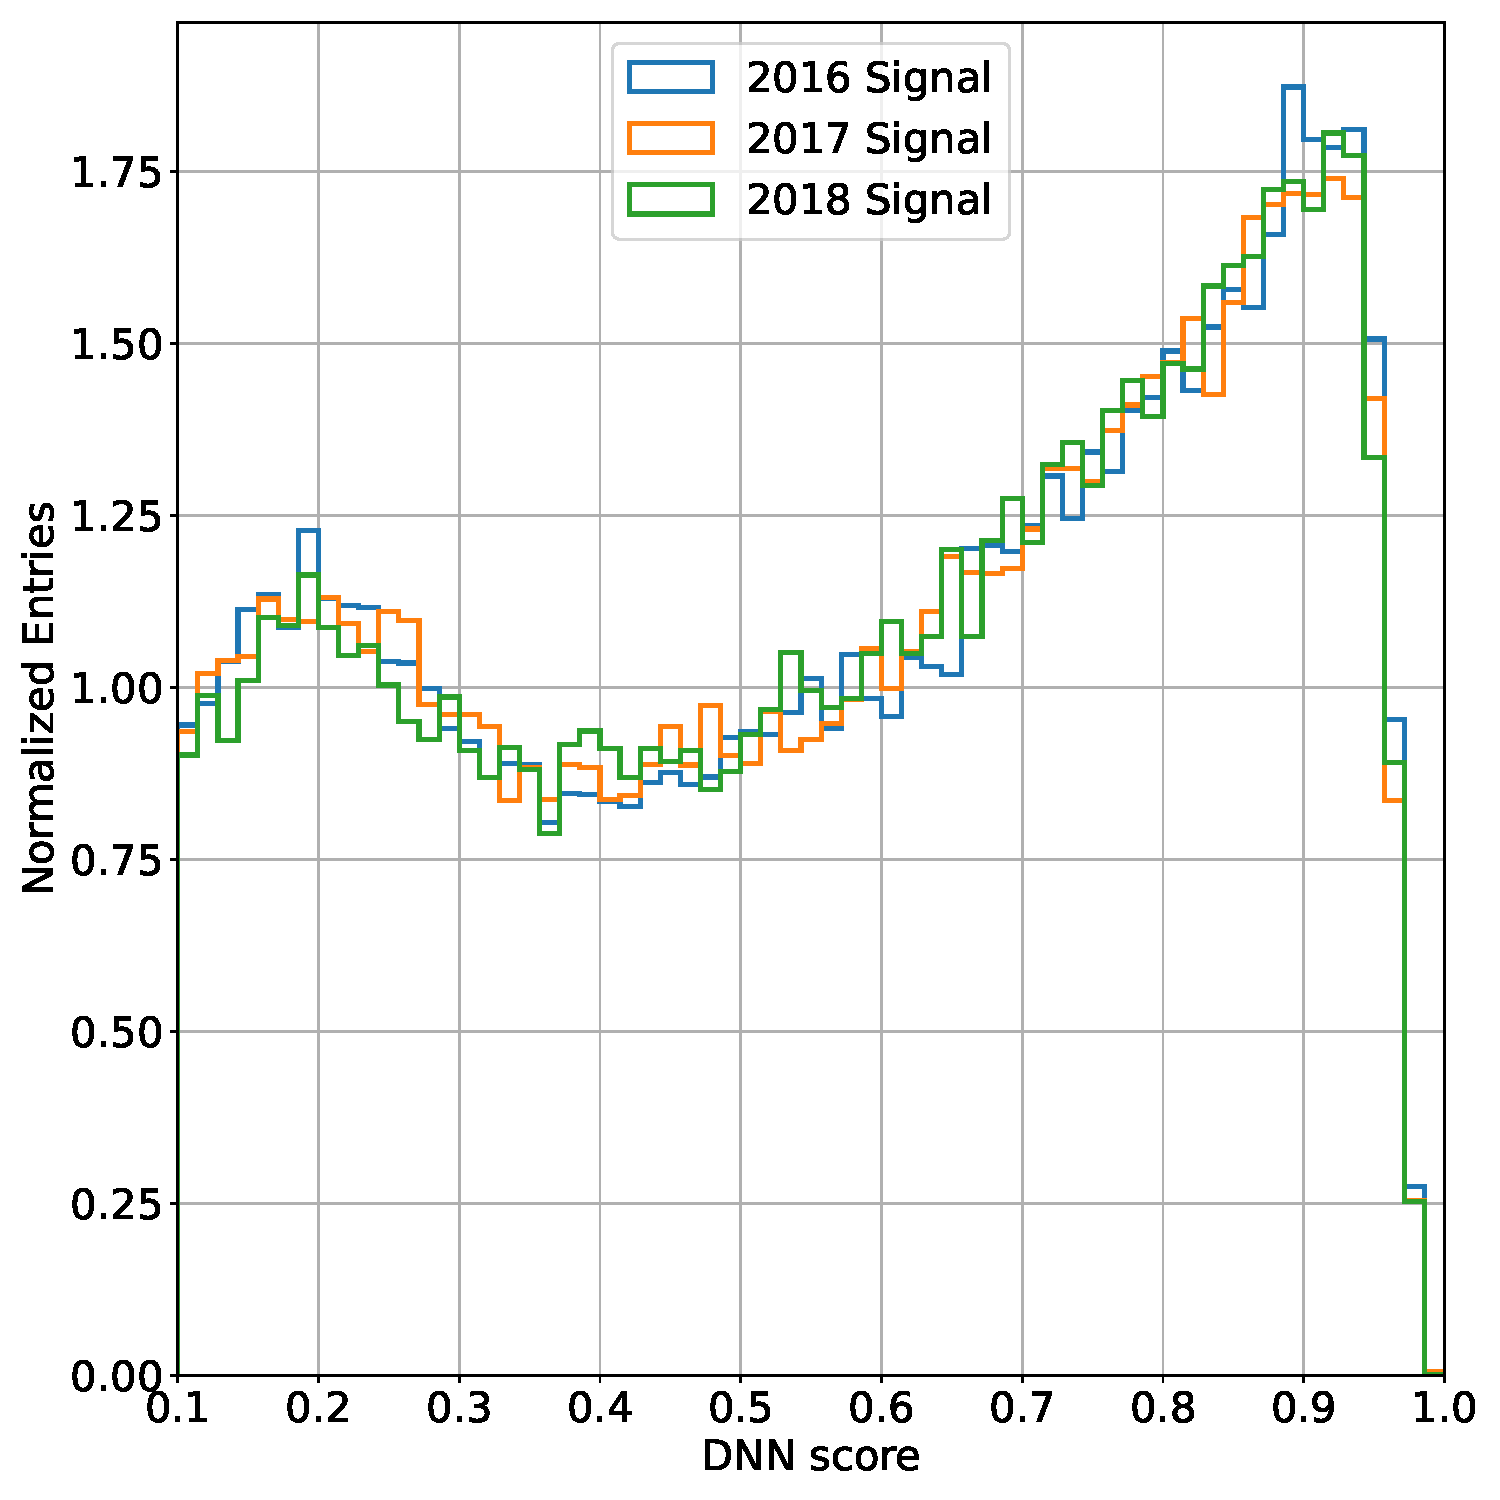
\includegraphics[width=0.45\textwidth]{Sections/HHWWgg/images/DNN/YearByYear_SLDNN_scores_sig.pdf}}
  \caption{DNN output score of data events in the sideband region (a), and HH simulation events in the signal region (b), for each separate year.}
  \label{fig:YearByYear_DNN_Scores}
\end{figure} 

% \begin{figure}[H]
%   \setcounter{subfigure}{0}
%   \centering
%   \subfloat[Without sideband scale]{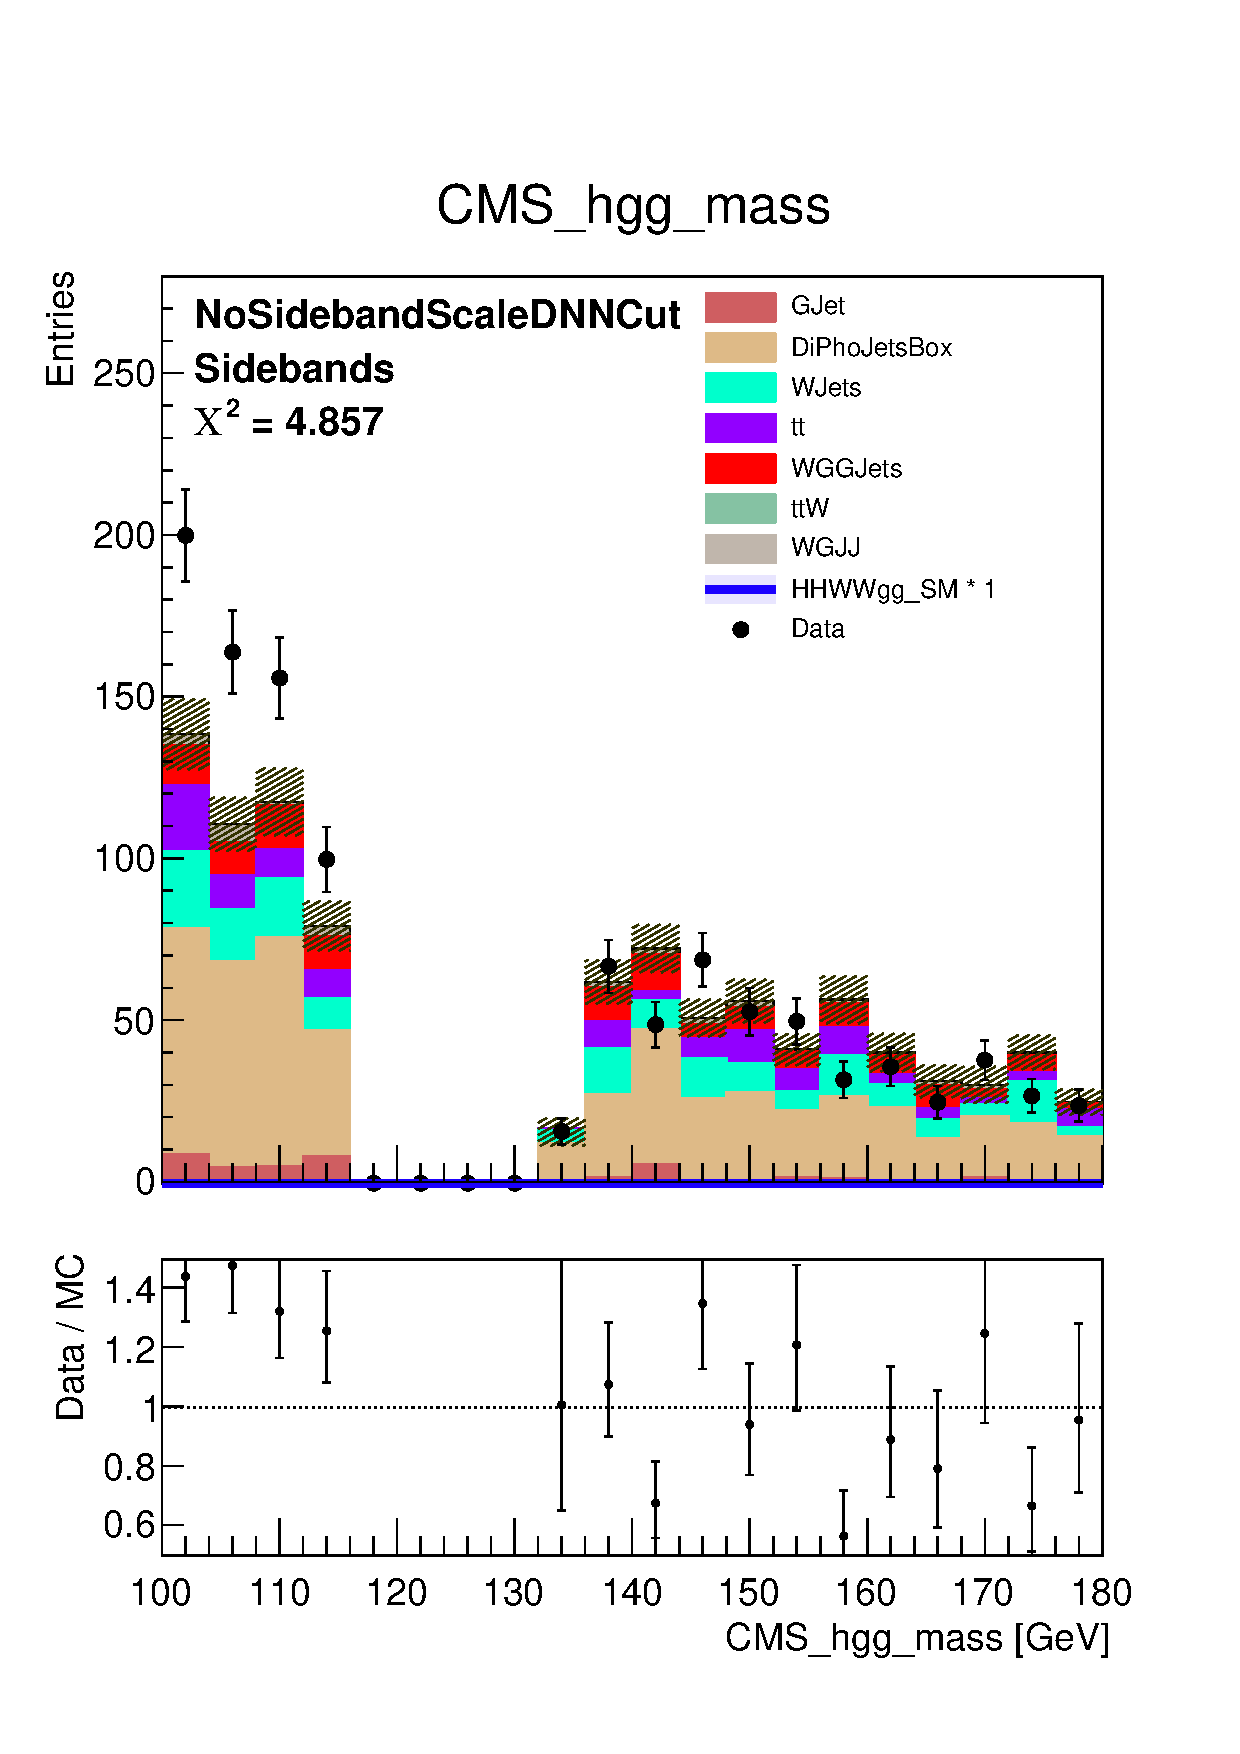
\includegraphics[width=0.45\textwidth]{Sections/HHWWgg/images/DNN/DataMC_CMS_hgg_mass_SB_NoSidebandScaleFactor_nonLog.pdf}}
%   \qquad
%   \subfloat[With sideband scale]{\includegraphics[width=0.45\textwidth]{Sections/HHWWgg/images/DNN/DataMC_CMS_hgg_mass_SB_WithSidebandScaleFactor_nonLog.pdf}}
%   \caption{data / MC ratio of DNN output score in the data sidebands before and after applying a sideband integral scaling factor of 1.140 to MC}
%   \label{fig:DNNSidebands_withAndWithoutSidebandScale}
% \end{figure} 

\clearpage 

\subsubsection{Standard Model: Categorization} \label{subsubsec:SLCategorization}

After computing a DNN output score for each event, events are placed into categories based on their DNN score in order to maximize the sensitivity of the DNN categorization. The optimization of categories 
is done using the output HH class DNN score only, as it has a known correlation to the H and continuum background DNN scores. If an event has a large HH class DNN score, by construction 
it must have small H and continuum background DNN output scores. 
Sensitivity is maximized by systematically determining the ideal position of category boundaries in terms of DNN score in order to maximize total significance, a 
proxy of the result of the asymptotic limits method to be applied during extraction of final results via fitting of the background models to the data.

This categorization is done using signal and background MC in the signal region,
and therefore is maximally optimial for data when data and MC fully agree in the dataside bands. After scaling MC in the sidebands to the integral of data in the sidebands, a non-optimal data-MC agreement is found. In order to correct for this disagreement, 
a per-bin reweighting of the DNN score is performed. The reweighting is performed using the Run 2 dataset and 2017 MC, with MC appropriately scaled to cross section, luminosity, 
PU reweight and any CMS POG (Physics object groups) recommended scale factors. Each DNN score bin weight is computed as the ratio of data to MC in the sideband region. The event weight is then applied to MC 
in the sideband and signal region events. It should be noted that this reweighting is used only to optimize analysis categories, and is not used for the evaluation of 
any final results. %The reweighted DNN score distributions is used to compute a per-event weight. 

During category optimization, generally a finner binning of the DNN score distributions leads to a greater significance. However, small bin widths can cause statistical fluctuations which 
bias categorization, as a very high (low) yield bin would improve (reduce) a potential category's significance drastically, thus biasing the categorization. To ensure that the 
effect of statistical fluctuations is reduced in the categorization procedure, a smoothing of the background distributions is performed. %using the Smooth-Super method of TGraphSmooth.

% The result of this smoothing can be seen in Figure \ref{fig:DNN-Smoothing}, where the median red line is used as the background distribution for categorization. In addition, 
% a $\pm 1\sigma$ Poissonian uncertainty is applied bin-by-bin to the smoothed distribution. This is done in order to demonstrate that most fluctuations are Poissonian in nature. 

The smoothing procedure is performed on background MC in the signal and side-band region. The smoothing procedure ensures that statistical fluctuations in the shape of the 
DNN scores have a negligible impact on the categorization procedure. 

% Events in the DNN discriminant distribution are separated into groups of bins ranging from DNN discriminant scores of 0.1 to 1. Events with a score of less than 0.1 are 
% not used for categorization. 

An optimal categorization of events based on the DNN discriminant variable is extracted by computing total significance among categories, varying the number of categories, number of equally sized bins, 
and definition of the signal region. A simultaneous optimization of category boundaries is performed, and the case which yields the greatest significance is chosen as the final categorization. Total significance is defined as the quadtratic sum of category 
significance, where category significance is defined by 
Equation \ref{eq:SignifianceDef} (Equation 96 in \cite{Cowan_2011}), where S and B are the number of weighted signal (HH events) and background (Single H $+$ continuum background) events in the category, respectively. Events with a score of less than 
0.1 are not used for categorization. 

\begin{equation} \label{eq:SignifianceDef}
  \sqrt{2((S + B)ln(1 + \frac{S}{B}) - S)}
\end{equation}

The optimal category boundaries for a given number of categories, equally sized bins and signal region window are chosen by computing total significance for every possible position of category boundaries 
given the number of bins and categories. A simultaneous optimization of category boundaries is performed. The category boundary positions which yield the greatest total significance are defined as the optimal category boundaries for the given number of categories,
bins and signal region window. 

The number of categories is varied from 1-5, and the number of equally sized bins is varied among: [10, 20, 30, 40, 50, 60, 70, 80, 90, 100, 110, 120, 130, 140, 150, 160, 170, 180, 190, 380, 760, 1520]. When computing significance 
values for category optimization, a signal region definition of 122 to 128 GeV is used as this is the experimental resolution: A range centered around the expected higgs mass with a width $\approx \pm$ 1-2 times the expected signal width,
known a-posteriori from analytic fitting. 

%, and the signal region window is varied
%among diphoton mass windows of (115, 135), (120, 130), (121, 129), (122, 128), and (123, 127). The signal region definition is varied because the significance computed in the di-photon mass range 115-135 may 
%not serve as the best proxy for the 95\% CL limit on di-Higgs cross section. 

The optimal categorization was chosen based on the 90 bin case, in which category boundaries are simultaneously optimized among 90 equally sized bins of width (1/90) from output DNN scores 
of 0.1 to 1. 

%It was also found that a signal region definition of 122 to 128 GeV in the di-photon mass region returns the greatest significance with number of bins and categories held constant,
%a hint that choosing optimal category boundaries based on this definiton may return the most sensitive result. 

% The expected signal region yields for background (simulated with MC reweighted to the data sidebands) and HH signal, both scaled to the Run 2 luminosity of 137 $fb^{-1}$, are shown in Figure \ref{fig:DnnScore} for the HH node DNN score. These distributions are 
% used for significance computations.    

A very small increase in total significance is obtained when increasing from four to five total categories, as seen in Figure \ref{fig:SigVsNcats}, in both the case where significance is computed with Equation \ref{eq:SignifianceDef}
and S / $\sqrt{B}$. In addition, the category boundary 
for the most sensitive category remains constant. Therefore, the choice is made to classify events into four categories. The category boundaries, number of signal events, number of background 
events and significance for the N category case where N ranges from 1-5 are shown in Tables \ref{tab:SLcategories_1}, \ref{tab:SLcategories_2}, \ref{tab:SLcategories_3}, \ref{tab:SLcategories_4} and \ref{tab:SLcategories_5},
where the final categorization is that shown in Table \ref{tab:SLcategories_4}. The HH yields in these tables, denoted by 'S', are properly scaled to the cross section and branching ratio of 
the Semi-Leptonic final state of HH$\rightarrow$WW$\gamma\gamma$. The MC modeling the backgound in the signal region comes from the continuum background MC which is smoothed before 
use in the category optimization. Each MC process is scaled to its cross section and branching ratio, as well as the kinematic weight with its fiducial selection, the removal of events with an absolute value of weight times kinematic 
weight $> 10$.

\newpage 

\begin{table}[H]
  \begin{center}
    \begin{tabular}{c|c|c|c|c|c|c}
    CatN & DNN Min & DNN Max & S & $B_{SR}$ & $Data_{Sideband}$ & Significance\\ \hline
    0 & 0.89 & 1.0 & 0.03568 & 0.81037 & 8.0 & 0.03935 \\ 
    \end{tabular}
  \end{center}
\caption{
    Semi-Leptonic DNN Category Boundaries and yields in signal region for 1 Categories
}
\label{tab:SLcategories_1}
\end{table}
 
\begin{table}[H]
  \begin{center}
    \begin{tabular}{c|c|c|c|c|c|c}
    CatN & DNN Min & DNN Max & S & $B_{SR}$ & $Data_{Sideband}$ & Significance\\ \hline
    0 & 0.89 & 1.0 & 0.03568 & 0.81037 & 8.0 & 0.03935 \\ 
    1 & 0.1 & 0.89 & 0.23129 & 511.65079 & 3580.0 & 0.01022 \\ 
    \end{tabular}
  \end{center}
\caption{
    Semi-Leptonic DNN Category Boundaries and yields in signal region for 2 Categories
}
\label{tab:SLcategories_2}
\end{table}
 
\begin{table}[H]
  \begin{center}
    \begin{tabular}{c|c|c|c|c|c|c}
    CatN & DNN Min & DNN Max & S & $B_{SR}$ & $Data_{Sideband}$ & Significance\\ \hline
    0 & 0.89 & 1.0 & 0.03568 & 0.81037 & 8.0 & 0.03935 \\ 
    1 & 0.64 & 0.89 & 0.09449 & 16.43561 & 114.0 & 0.02329 \\ 
    2 & 0.1 & 0.64 & 0.1368 & 495.21518 & 3466.0 & 0.00615 \\ 
    \end{tabular}
  \end{center}
\caption{
    Semi-Leptonic DNN Category Boundaries and yields in signal region for 3 Categories
}
\label{tab:SLcategories_3}
\end{table}
 
\begin{table}[H]
  \begin{center}
    \begin{tabular}{c|c|c|c|c|c|c}
    CatN & DNN Min & DNN Max & S & $B_{SR}$ & $Data_{Sideband}$ & Significance\\ \hline
    0 & 0.89 & 1.0 & 0.03568 & 0.81037 & 8.0 & 0.03935 \\ 
    1 & 0.84 & 0.89 & 0.02267 & 1.84053 & 12.0 & 0.01668 \\ 
    2 & 0.63 & 0.84 & 0.07483 & 15.73924 & 111.0 & 0.01885 \\ 
    3 & 0.1 & 0.63 & 0.13379 & 494.07101 & 3457.0 & 0.00602 \\ 
    \end{tabular}
  \end{center}
\caption{
    Semi-Leptonic DNN Category Boundaries and yields in signal region for 4 Categories
}
\label{tab:SLcategories_4}
\end{table}
 
\begin{table}[H]
  \begin{center}
    \begin{tabular}{c|c|c|c|c|c|c}
    CatN & DNN Min & DNN Max & S & $B_{SR}$ & $Data_{Sideband}$ & Significance\\ \hline
    0 & 0.89 & 1.0 & 0.03568 & 0.81037 & 8.0 & 0.03935 \\ 
    1 & 0.84 & 0.89 & 0.02267 & 1.84053 & 12.0 & 0.01668 \\ 
    2 & 0.64 & 0.84 & 0.07182 & 14.59508 & 102.0 & 0.01878 \\ 
    3 & 0.25 & 0.64 & 0.0964 & 157.99225 & 974.0 & 0.00767 \\ 
    4 & 0.1 & 0.25 & 0.0404 & 337.22293 & 2492.0 & 0.0022 \\ 
    \end{tabular}
  \end{center}
\caption{
    Semi-Leptonic DNN Category Boundaries and yields in signal region for 5 Categories
}
\label{tab:SLcategories_5}
\end{table}

\newpage 

\begin{figure}[H]
  \setlength{\unitlength}{1mm}
  \begin{center}
    \mbox{\includegraphics*[height=100mm]{Sections/HHWWgg/images/DNN/Categorization/SigVsNCats.pdf}
    }
  \end{center}
  \caption{Total significance vs. number of categories in DNN categorization optimization, using either Equation \ref{eq:SignifianceDef} or S / $\sqrt{B}$ to 
  compute each category's significance, with total significance computed as category significances summed in quadrature. S is the number of weighted HH events, 
  and B is the weghted number of MC events modeling the continuum background in the signal region plus the number of weighted single H events. Also shown in Table \ref{tab:SigVsNcats_table}}    
  \label{fig:SigVsNcats}
\end{figure}

\begin{table}[H]
  \begin{center}
    \begin{tabular}{c|c|c}
    NCategories & Total Significance with Eq \ref{eq:SignifianceDef} & $\frac{S}{\sqrt{B}}$ \\ \hline
    1 & 0.03935 & 0.039635  \\ 
    2 & 0.040656 & 0.040933  \\ 
    3 & 0.046135 & 0.04639  \\ 
    4 & 0.047095 & 0.047352  \\ 
    5 & 0.04736 & 0.047616  \\ 
    \end{tabular}
  \end{center}
\caption{
    Significance values using two equations for significance
}
\label{tab:SigVsNcats_table}
\end{table}

\clearpage

\subsubsection{EFT Benchmarks: Parametric Binary Deep Neural Network}

To categorize events from the 20 EFT benchmarks in the Semi-Leptonic final state, a parametric binary DNN is used. The DNN is trained using 2017 signal and background samples, and 
is evaluated on 2016, 2017 and 2018 signal samples for analytic fitting and on Run 2 data to be used for categorization and data-driven background modeling. 
Models of the 20 EFT benchmarks are obtained by reweighting the combination of four NLO samples to each benchmark at NLO precision. The 20 EFT benchmark samples are combined and considered together as signal. 
The network is then trained on a labelled dataset with the 20 EFT HH processes as the signal, 
and various background process labelled as background. 

In addition to the training variables used for the multiclass DNN, the node number ranging from 1-20 is input as a feature into the DNN, allowing one to produce an output score for 
any EFT benchmark hypothesis. This is essentially a way to produce 20 MVA scores in a given training, which is much more convenient than running 20 individual trainings.

% The samples used for training and labeled as signal are the 12 LO benchmark samples with 2017 detector conditions. When training on these samples, the same reweighting 
% procedure described in the multi-class DNN is followed, where in this case samples are reweighted to the NLO precision of their corresponding benchmark rather than 
% the standard model at NLO precision. 

The same training pre-selections are applied in this case as for the multi-class DNN, and the same category boundary optimization procedure is followed. 

\clearpage

% Fully-Hadronic
\subsection{Fully-Hadronic} \label{subsec:FullyHadronicEventSelection}

Data and simulation events fall into the Fully-hadronic category if they contain at least 4 jets satisfying the conditions described in Section \ref{sec:Jets}, and at least one diphoton candidate satisfying the selections described in Section \ref{sec:photons}. To maintain categorical orthogonality with the Semi-leptonic and Fully-leptonic final states, events in the Fully-hadronic category are required to have exactly zero leptons passing the
selections described in Section \ref{sec:LeptonSelections}. 

Because the invariant mass resolution of two jets is not expected to be precise enough to separate W-boson and Z-boson events, the Fully-Hadronic $HH \rightarrow ZZ\gamma\gamma$
channel is expected to overlap with the Fully-hadronic $HH \rightarrow WW\gamma\gamma$ channel. In addition, the HH$\rightarrow$bb$\gamma\gamma$ process is difficult to distinguish from the Fully-hadronic HH$\rightarrow$VV$\gamma\gamma$ signatures. In order to optimize this final state analysis for the Fully-hadronic WW$\gamma\gamma$ final state, a dedicated ``bb$\gamma\gamma$ killer'' DNN is trained to differentiate HH$\rightarrow$bb$\gamma\gamma$ from all backgrounds. After the removal of these additional final states, any remaining events are included in the signal definition.
Therefore, in the final signal definition, $HH \rightarrow ZZ\gamma\gamma \rightarrow qqqq\gamma\gamma$, $HH \rightarrow bb\gamma\gamma$ and $HH \rightarrow WW\gamma\gamma \rightarrow qqqq\gamma\gamma$ are included. Thus, the Fully-Hadronic signal corresponds to $HH \rightarrow (WW + ZZ + bb) \gamma \gamma$. 

% Note, that we applied bb$\gamma \gamma$ killer cut before adding bb$\gamma \gamma$ signal.

% To avoid the overlap consideration, the $HH \rightarrow ZZ\gamma\gamma \rightarrow qqqq\gamma\gamma$
% process is included in the analysis' signal definition.
% Therefore, the Fully-Hadronic signal corresponds to $HH \rightarrow (WW + ZZ)\gamma\gamma \rightarrow qqqq\gamma\gamma$.

% Because the WW and ZZ yields are combined, the fullyhadronic selections described above and in this section are applied to both the WW and ZZ signal samples.

% As a combination is foreseen with all nonresonant HH channels, including bb$\gamma\gamma$, it is ideal to minimize the number of bb$\gamma\gamma$ events falling into both analysis phase spaces as much as possible, to reduce
% the likelihood that data events pass both analysis selections.

% This is because if data events fall into both analysis phase spaces, they must be handled appropriately in the
% combination, otherwise the events would be incorrectly double counted when deriving a combined result. 

\subsubsection{DNN for Fully-Hadronic Channel}
\label{subsubsec:FullyHadronicDNN}
As mentioned in Section \ref{sec:Strategy}, a DNN approach must be taken for the Fully-hadronic final state to optimize sensitivity, while simultaneously minimizing
contamination from the $HH \rightarrow (bb + ZZ)\gamma\gamma$ processes. To this end, two binary trainings are performed as follows:

\begin{itemize}
  \item \textbf{WW$\gamma\gamma$ identifier}: Trained for the separation of signal ($HH \rightarrow WW\gamma\gamma$) and backgrounds listed in Tab.~\ref{tab:fullyHadronicMCBkg}).
  \item \textbf{bb$\gamma\gamma$ killer}: Trained in order to obtain a discriminant to use for reducing the contamination of bb$\gamma\gamma$. For this training, bb$\gamma\gamma$ is considered signal,
  and the MC listed in Tab.~\ref{tab:fullyHadronicMCBkg}, with the addition of the WW$\gamma\gamma$ process, are considered background.
\end{itemize}
\begin{table}[!htbp]
  \begin{center}
          \begin{tabular}{|c|}
                \hline
                \textbf{MC Samples}  \\ \hline
                DiPhoJetsBox\_MGG-80toInf  \\ \hline
                GJet\_40toInf $\Rightarrow$ Data-Driven QCD \\ \hline
                HT-binned QCD  $\Rightarrow$ Data-Driven QCD\\ \hline
                tt$\gamma\gamma+$0Jets  \\ \hline
                tt$\gamma+$Jets  \\ \hline
                % ttH  \\ \hline
                % VH   \\ \hline
                % VBF-H    \\ \hline
                % GluGluH \\ \hline
          \end{tabular}
  \caption{MC list for Fully-Hadronic}
  \label{tab:fullyHadronicMCBkg}
  \end{center}
\end{table}

\subsubsection{WW$\gamma\gamma$ identifier}

This binary DNN training is used for the separation of di-Higgs (WW$\gamma\gamma$) signal w.r.t. background. The backgrounds used for the Fully-Hadronic
training is shown in Tab.~\ref{tab:fullyHadronicMCBkg}.

From the list of background considered in Tab.~\ref{tab:fullyHadronicMCBkg}, QCD simulation suffers from a very low number of events, so a data-driven approach is considered for estimating the QCD. The considered data-driven approach estimates QCD and $\gamma$+jets simultaneously. This is described in sec.~\ref{subsubsec:QCDDataDriven}.

This DNN is trained using 2017 signal and background MC, and is evaluated on the signal and data of each data-taking year. The sum of three EFT benchmark simulation samples generated at LO (nodes 1, 2 and 3 as defined in Table \ref{tab:eft_bench}) is considered as signal in MC training, and is reweighted to the SM HH signal and NLO as was done in the Semi-leptonic case. The dominant background processes, namely $\gamma\gamma+$jets and QCD are used as background for training the network.

% The events used to train the network are required to pass the common di-Photon pre-selection described in Sec.~\ref{sec:commomSel} 

In order to produced a data-driven estimate of QCD$+\gamma$jet, data events in the sideband with an additional selection on photon ID of $<$ -0.7 is applied to the leading and subleading photons. Therefore, events used for the Fully-hadronic DNN training are required to have a photon ID score $>$ -0.7. 

% along with the photon ID $>$ -0.7 (for both leading and subleading photons), contains exactly zero leptons passing the common lepton selections in Sec.~\ref{sec:LeptonSelections}, at least 4 jets in Sec.~\ref{subsec:Jets}.

The features used as input to the Fully-Hadronic channel DNN can be found in Tab.~\ref{tab:FHDNNinputfeatures1} and Tab.~\ref{tab:FHDNNinputfeatures2}.

\begin{table}[!htbp]
\centering
% \resizebox{\textwidth}{!}
{
% \begin{tabular}{| l | l |}
\begin{tabular}{|p{4cm}|p{12cm}|}
\hline
Feature & Description \\
\hline
Leading Photon pT / \mgg& pT of the photon with the highest transverse momentum out of the selected photons, scaled to diphoton mass. \\
Subleading Photon pT  / \mgg& pT of the photon with the second highest transverse momentum out of the selected photons, scaled to diphoton mass. \\
Leading Photon $\phi$ & Direction in the transverse plane of the photon with the highest transverse momentum out of the selected photons \\
Subleading Photon $\phi$ & Direction in the transverse plane of the photon with the second highest transverse momentum out of the selected photons \\
Leading Photon $\eta$ & Direction in the transverse plane of the photon with the highest transverse momentum out of the selected photons \\
Subleading Photon $\eta$ & Direction in the transverse plane of the photon with the second highest transverse momentum out of the selected photons \\
max Photon ID & The maximum value of the photon MVA score out of the two selected photons.\\
min Photon ID & The minimum value of the photon MVA score out of the two selected photons.\\

$\Delta \phi(\gamma \gamma)$ & Azimuthal separation between the two selection photon candidates\\
$\Delta R(\gamma \gamma)$ & Separation between two photons in the transverse plane\\

Jet Multiplicity & Number of selected jets in the event (flavour inclusive) \\
Sum two max bScores & Sum of two highest b-score jets out of all available good jets \\

Leading Jet p$_T$ & Transverse momentum of the jet with the highest transverse momentum out of the selected jets \\
Leading Jet $\eta$ & Rapidity of the jet with the highest transverse momentum out of the selected jets \\
Leading Jet $\phi$ & Phi of the jet with the highest transverse momentum out of the selected jets \\
Leading Jet E & Energy of the jet with the highest transverse momentum out of the selected jets \\
Leading Jet DeepJet Score & DeepJet b-tag discriminator score of the jet with the highest transverse momentum out of the selected jets \\

Subleading Jet p$_T$ & Transverse momentum of the jet with the second highest transverse momentum out of the selected jets \\
Subleading Jet $\eta$ & Rapidity of the jet with the second highest transverse momentum out of the selected jets \\
Subleading Jet $\phi$ & Phi of the jet with the second highest transverse momentum out of the selected jets \\
Subleading Jet E & Energy of the jet with the second highest transverse momentum out of the selected jets \\
Subleading Jet DeepJet Score & DeepJet b-tag discriminator score of the jet with the second highest transverse momentum out of the selected jets \\
% \hline\hline
% \endlastfoot
\hline
\end{tabular}
}

\caption{Input features used to train Fully-Hadronic channel DNN. \label{tab:FHDNNinputfeatures1}}
\end{table}

\begin{table}[!htbp]
\centering
% \resizebox{\textwidth}{!}
{
% \begin{tabular}{| l | l |}
\begin{tabular}{|p{4cm}|p{12cm}|}
\hline
Feature & Description \\
\hline
Second Subleading Jet p$_T$ & Transverse momentum of the jet with the third highest transverse momentum out of the selected jets \\
Second Subleading Jet $\eta$ & Rapidity of the jet with the third highest transverse momentum out of the selected jets \\
Second Subleading Jet $\phi$ & Phi of the jet with the third highest transverse momentum out of the selected jets \\
Second Subleading Jet E & Energy of the jet with the third highest transverse momentum out of the selected jets \\
Second Subleading Jet DeepJet Score & DeepJet b-tag discriminator score of the jet with the third highest transverse momentum out of the selected jets \\

Third Subleading Jet p$_T$ & Transverse momentum of the jet with the fourth highest transverse momentum out of the selected jets \\
Third Subleading Jet $\eta$ & Rapidity of the jet with the fourth highest transverse momentum out of the selected jets \\
Third Subleading Jet $\phi$ & Phi of the jet with the fourth highest transverse momentum out of the selected jets \\
Third Subleading Jet E & Energy of the jet with the fourth highest transverse momentum out of the selected jets \\
Third Subleading Jet DeepJet Score & DeepJet b-tag discriminator score of the jet with the fourth highest transverse momentum out of the selected jets \\

$\Delta \phi(HH)$ & Azimuthal separation between the two selection Higgs candidates\\
$\Delta R(HH)$ & Separation between two Higgs in the transverse plane\\
$min(\Delta R(g_k,j_l))$ & minimum separation between the selected jet and photon candidate\\
$max(\Delta R(g_k,j_l))$ & maximum separation between the selected jet and photon candidate\\
$min(\Delta R(j_k,j_l))$ & minimum separation between the jet candidates\\
$max(\Delta R(j_k,j_l))$ & maximum separation between the jet candidates\\
costhetastar & The angle between the parton collision axis $z$ and the $pp\rightarrow H_1H_{2}$ decay axis $z'$, both defined in the $H_1H_{2}$ system rest frame \\
costheta1 & Angle between the direction of the W-boson ($W_1$) from the $H_1\rightarrow W_1 W_2$ and the direction opposite the $H_1H_2$ in the $H_1$ rest frame.\\
costheta2 & Angle between the direction of the W-boson ($W_2$) from the $H_2\rightarrow \gamma \gamma$ and the direction opposite the $H_1H_2$ in the $H_2$ rest frame.\\
Phi & Angle between the decay planes of the two Z-system in the $H_1H_2$ rest frame\\
Phi1 & Angle between the $zz'$ plane and the plane of the $H_{1}\rightarrow \gamma \gamma$ decay in the $H_{1}H_{2}$ rest frame \\
W1 pT & pT of vector sum of two leading jets\\
W1 $\eta$ &  rapidity of vector sum of two leading jets\\
W1 mass &  Invariant mass of vector sum of two leading jets\\

W2 pT & pT of vector sum of 3rd and 4th leading jets\\
W2 $\eta$ & rapidity of vector sum of 3rd and 4th leading jets\\
W2 mass & Invariant mass of vector sum of 3rd and 4th leading jets\\

WW pT & pT of vector sum of first four leading jets\\
WW $\eta$ & rapidity of vector sum of first four leading jets\\
WW mass & Invariant mass of vector sum of first four leading jets\\
\hline
\end{tabular}
}

\caption{Input features used to train Fully-Hadronic channel DNN. \label{tab:FHDNNinputfeatures2}}
\end{table}

The data/MC agreement is shown for a few leading importance input features, after the removal of events with a DNN score $<$ 0.1, in Figures \ref{fig:FH_DataMC_1} and \ref{fig:FH_DataMC_2}. 

\begin{figure}[!htbp]
  \centering
  \includegraphics[width=0.45\textwidth]{Sections/HHWWgg/images/FH_DNN/DataMC/DataMC_New_DR_gg_SB_log.pdf}%
  \includegraphics[width=0.45\textwidth]{Sections/HHWWgg/images/FH_DNN/DataMC/DataMC_Scaled_Leading_Photon_pt_SB_log.pdf}%
  \caption{Data/MC comparison of a fully-hadronic leading DNN input feature (left) and second leading DNN input feature (right).}
\label{fig:FH_DataMC_1}
\end{figure}

\begin{figure}[!htbp]
  \centering
  \includegraphics[width=0.45\textwidth]{Sections/HHWWgg/images/FH_DNN/DataMC/DataMC_New_pTBasedSel_WW_pT_SB_log.pdf}%
  \includegraphics[width=0.45\textwidth]{Sections/HHWWgg/images/FH_DNN/DataMC/DataMC_evalDNN_WWvsAll_SB_log.pdf}%
  \caption{Data/MC comparison of a fully-hadronic third leading DNN input feature and DNN score.}
\label{fig:FH_DataMC_2}
\end{figure}


% The correlation between all input features is checked and shown in Fig.~\ref{fig:FH_DNN_CorrelationPlot}. For some of input features there are large correlations but for DNN it should not affect the result. So, variables having large correlations are not removed.

% \begin{figure}[!htbp]
%   \centering 
%   \includegraphics[width=0.5\textwidth]{Images/Logos/CMS_Logo.png}
% %   \includegraphics[width=\textwidth,trim={17cm 17cm 0 0},clip=true]{Sections/HHWWgg/images/FH_DNN/WWgg/correlation_plot.pdf}  
%   \caption{Correlation of Fully-Hadronic DNN WW$\gamma \gamma$ identifier training input features}
%   \label{fig:FH_DNN_CorrelationPlot}
% \end{figure}

% The DNN network optimized hyperparameter setting can be found in Tab.~\ref{tab:FH_DNN_HyperparameterSettings} and the one of best architecture that we investigated for the Fully-Hadronic channel, can be found in Fig.~\ref{fig:FH_DNN_Architecture}.
% \begin{table}[!htbp]
% \centering
% \caption{Hyper-parameter settings for WW$\gamma \gamma$ identifier training for the Fully-Hadronic channel DNN}
% % \resizebox{\textwidth}{!}
% {
% \begin{tabular}{| l | l |}
% \hline
% Hyper-Parameter & Settings \\
% \hline
% Epoch & 170 \\
% Learning rate & $10^{-3}$ \\
% Batch size & 250 \\
% % Dropout rate & 0.1 \\
% Optimizer & Nadam \\
% Loss function & categorical crossentropy \\
% Kernel initialiser & glorot normal \\
% Hidden layer activation function & elu \\
% Output layer activation function & softmax \\ \hline
% \end{tabular}
% }
% \label{tab:FH_DNN_HyperparameterSettings}
% \end{table}

% \begin{figure}[!htbp]
%   \centering
%   \includegraphics[height=0.5\textwidth]{Sections/HHWWgg/images/FH_DNN/WWgg/model_schematic.png}
%   % \includegraphics[height=0.5\textwidth,trim={0 30cm 0 0},clip=true]{Sections/HHWWgg/images/FH_DNNmodel_schematic.png}%
%   % \includegraphics[height=0.5\textwidth,trim={0 0 0 35cm},clip=true]{Sections/HHWWgg/images/FH_DNNmodel_schematic.png}
%   \caption{DNN network architecture. This architecture is used by both training - a) WW$\gamma \gamma$ identifier, and b) bb$\gamma \gamma$ killer.}
%   \label{fig:FH_DNN_Architecture}
% \end{figure}
% \begin{figure}[!htbp]
%   \centering
%   \includegraphics[height=\textheight]{Sections/HHWWgg/images/FH_DNNmodel_schematic.png}%
%   \caption{Correlation of Fully-Hadronic DNN input features}
%   \label{fig:FH_DNN_Architecture1}
% \end{figure}

The output ROC curve from the training is shown in Fig.~\ref{fig:FH_DNN_ROC}.

% and couple of other metrics are shown in Fig.~\ref{fig:FH_DNN_Metrics}. 

As the curves are similar, this indicates no sign of over-training. Additionally, the output score of signal and background for training and testing shows no overtraining signature, as shown in Fig.~\ref{fig:FH_DNN_OutputScore}.

In addition, a check is performed in a dedicated control region to demonstrate that a large difference in data and MC acceptance is not expected to be introduced by the
WW$\gamma\gamma$ identifier DNN, and that the DNN behaves as expected on its signal topology. This check is shown in Appendix \ref{sec:DNN_and_signal_validation}.

\begin{figure}[!htbp]7
  \centering
  \includegraphics[scale=0.4]{Sections/HHWWgg/images/FH_DNN/WWgg/ROC.pdf}%
  \caption{ROC curve for WW$\gamma\gamma$ identifier Fully-Hadronic DNN}
  \label{fig:FH_DNN_ROC}
\end{figure}

% \begin{figure}[!htbp]
%   \centering
%   % \includegraphics[width=0.7\textwidth]{Sections/HHWWgg/images/FH_DNNall_metrics_nomgg.pdf}%
%   \includegraphics[scale=0.4]{Sections/HHWWgg/images/FH_DNN/WWgg/all_metrics.pdf}%
%   \caption{Metrics for Fully-Hadronic DNN WW$\gamma \gamma$ identifier. Loss w.r.t. epoch(top left). Precision-Recall curve w.r.t. epoch. Precision is defined as $\frac{(TruePositive)}{(TruePositive)+(FalsePositive)}$ and recall is defined as $\frac{(TruePositive)}{(TruePositive)+(FalseNegative)}$(top right). Precision w.r.t. epoch (bottom left). Recall w.r.t. epoch (bottom right).}
%   \label{fig:FH_DNN_Metrics}
% \end{figure}

\begin{figure}[!htbp]
  \centering
  \includegraphics[scale=0.6]{Sections/HHWWgg/images/FH_DNN/WWgg/overfitting_plot_BinaryClassifier_Binary.png}%
  \caption{Output score of Fully-Hadronic DNN WW$\gamma \gamma$ identifier training}
  \label{fig:FH_DNN_OutputScore}
\end{figure}

\subsubsection{bb$\gamma\gamma$ killer}

This binary DNN training is used as a bb$\gamma\gamma$ killer. The objective of this DNN is to output a bb$\gamma\gamma$ killer score to use as a discriminant to use for the removal of bb$\gamma\gamma$ events from the WW$\gamma\gamma$ phase-space. This is trained considering a bb$\gamma\gamma$ simulation sample as signal. The list of background used consists of all background mentioned in Tab.~\ref{tab:fullyHadronicMCBkg} along with the Fully-hadronic WW$\gamma\gamma$ simulation sample. Other details for this training including the events selections, list of input variables and DNN architecture remain the same as for the WW$\gamma\gamma$ identifier described in Section \ref{subsubsec:FullyHadronicDNN}. 

% The correlation between all the input features are checked and shown in Fig.~\ref{fig:FH_DNN_CorrelationPlot_bbggVsAll}. For some of input features there are large correlations but for DNN it should not affect the result. So, variables having large correlations are not removed.
% \begin{figure}[!htbp]
%   \centering 
%   \includegraphics[width=0.5\textwidth]{Images/Logos/CMS_Logo.png}
% %   \includegraphics[width=\textwidth,trim={17cm 17cm 0 0},clip=true]{Sections/HHWWgg/images/FH_DNN/WWgg/correlation_plot.pdf}  
% %   \includegraphics[width=\textwidth,trim={17cm 17cm 0 0},clip=true]{Sections/HHWWgg/images/FH_DNN/BBgg/correlation_plot.pdf}
%   \caption{Correlation of Fully-Hadronic DNN bb$\gamma \gamma$ killer input features}
%   \label{fig:FH_DNN_CorrelationPlot_bbggVsAll}
% \end{figure}

% The DNN network optimized hyperparameter setting can be found in Tab.~\ref{tab:FH_DNN_HyperparameterSettings_bbggVsAll} and the one of best architecture that we investigated is same as used in Training -1, i.e. Fig.~\ref{fig:FH_DNN_Architecture}.
% \begin{table}[!htbp]
% \centering
% \caption{Hyper-parameter settings for bb$\gamma \gamma$ killer training for Fully-Hadronic channel}
% % \resizebox{\textwidth}{!}
% {
% \begin{tabular}{| l | l |}
% \hline
% Hyper-Parameter & Settings \\
% \hline
% Epoch & 400 \\
% Learning rate & $10^{-4}$ \\
% Batch size & 150 \\
% % Dropout rate & 0.1 \\
% Optimizer & Adam \\
% Loss function & categorical crossentropy \\
% Kernel initialiser & glorot normal \\
% Hidden layer activation function & elu \\
% Output layer activation function & softmax \\ \hline
% \end{tabular}
% }
% \label{tab:FH_DNN_HyperparameterSettings_bbggVsAll}
% \end{table}



% \begin{figure}[!htbp]
%   \centering
%   \includegraphics[height=0.5\textwidth]{Sections/HHWWgg/images/FH_DNN/BBgg/model_schematic.png}
%   % \includegraphics[height=0.5\textwidth,trim={0 30cm 0 0},clip=true]{Sections/HHWWgg/images/FH_DNN/BBgg/model_schematic.png}%
%   % \includegraphics[height=0.5\textwidth,trim={0 0 0 35cm},clip=true]{Sections/HHWWgg/images/FH_DNN/BBgg/model_schematic.png}
%   \caption{DNN network architecture}
%   \label{fig:FH_DNN_Architecture_bbggVsAll}
% \end{figure}
% \begin{figure}[!htbp]
%   \centering
%   \includegraphics[height=\textheight]{Sections/HHWWgg/images/FH_DNNmodel_schematic.png}%
%   \caption{Correlation of Fully-Hadronic DNN input features}
%   \label{fig:FH_DNN_Architecture1_bbggVsAll}
% \end{figure}

The output ROC curve of this training is shown in Fig.~\ref{fig:FH_DNN_ROC_bbggVsAll}. As the curves are similar for both the training and test datasets, this indicates that there is no overtraining. Additionally, the output score of signal and background for training and testing shows no overtraining signature,
as shown in Fig.~\ref{fig:FH_DNN_OutputScore_bbggVsAll}.

% and couple of other metrics are shown in Fig.~\ref{fig:FH_DNN_Metrics_bbggVsAll}.


% All of them shows no sign of over-training. Also, the output score of signal and background for training and testing shows no overtraining signature,
% as shown in Fig.~\ref{fig:FH_DNN_OutputScore_bbggVsAll}.

\begin{figure}[!htbp]
  \centering
  \includegraphics[scale=0.4]{Sections/HHWWgg/images/FH_DNN/BBgg/ROC.pdf}%
  \caption{ROC curve for Fully-Hadronic DNN bb$\gamma \gamma$ killer}
  \label{fig:FH_DNN_ROC_bbggVsAll}
\end{figure}

% \begin{figure}[!htbp]
%   \centering
%   % \includegraphics[width=0.7\textwidth]{Sections/HHWWgg/images/FH_DNNall_metrics_nomgg.pdf}%
%   \includegraphics[scale=0.4]{Sections/HHWWgg/images/FH_DNN/BBgg/all_metrics.pdf}%
%   \caption{Metrics for Fully-Hadronic DNN bb$\gamma \gamma$ killer. Loss w.r.t. epoch(top left). Precision-Recall curve w.r.t. epoch. Precision is defined as $\frac{(TruePositive)}{(TruePositive)+(FalsePositive)}$ and recall is defined as $\frac{(TruePositive)}{(TruePositive)+(FalseNegative)}$(top right). Precision w.r.t. epoch (bottom left). Recall w.r.t. epoch (bottom right).}
%   \label{fig:FH_DNN_Metrics_bbggVsAll}
% \end{figure}

\begin{figure}[!htbp]
  \centering
  \includegraphics[scale=0.6]{Sections/HHWWgg/images/FH_DNN/BBgg/overfitting_plot_BinaryClassifier_Binary.png}%
  \caption{Output score of Fully-Hadronic DNN bb$\gamma \gamma$ killer training}
  \label{fig:FH_DNN_OutputScore_bbggVsAll}
\end{figure}

\clearpage

% @Author: Ram Krishna Sharma
% @Date:   2021-05-18
% @Last Modified by:   Ram Krishna Sharma
% @Last Modified time: 2021-05-27
\subsubsection{Categorization}
\label{subsubsec:Categorization}

Events falling into the Fully-hadronic category are categorized in a similar fasion as described in Section \ref{subsubsec:SLCategorization} for the Semi-leptonic channel, but with the addition of a selection on the bb$\gamma\gamma$ killer score. 

% The categorization is performed in a similar way as described in sec.~\ref{subsubsec:SLCategorization}, for Semi-Leptonic channel.

The expected signal region yields background processes, simulated with MC, and HH signal, both scaled to the Run 2 luminosity of 137 $fb^{-1}$ (the estimated luminosity value at the time of training), are shown in Figure \ref{fig:FH_DnnScore}
for the WW$\gamma\gamma$ identifier score.

\begin{figure}[!htbp]
  \centering
  % \includegraphics[scale=0.6]{Sections/HHWWgg/images/FH_DNN/evalDNN.pdf}
  \includegraphics[scale=0.6]{Sections/HHWWgg/images/FH_DNN/WWvsAll_2017_NormUnity_BBggScoreCut0p6.pdf}
  \caption{Fully-Hadronic output score for signal and background. All distributions are normalized to unity.}
  \label{fig:FH_DnnScore}
\end{figure}

These distributions are used for significance computations. 

In performing the categorization, the same method is followed as for the semi-leptonic final state described in Section \ref{subsubsec:SLCategorization}. The result of smoothing of the MC in the signal region is shown in Fig.~\ref{fig:FH_smoothing}.

\begin{figure}[!htbp]
  \centering
  \includegraphics[scale=0.6]{Sections/HHWWgg/images/FH_DNN/h_DNN_bkg_SR_weighted_smoothing_SmoothSuper_nBins_50_massMin121_0_massMax129_0.pdf}
  \caption{Result of background smoothing for Fully-Hadronic channel.}
  \label{fig:FH_smoothing}
\end{figure}

The optimal categorization was chosen based on the 380 bin case, in which category boundaries are simultaneously optimized among 380 equally sized bins of width (1/380) from output WW$\gamma\gamma$ identifier DNN scores of 0.1 to 1.
It was also found that a signal region definition of 120 to 130 GeV in the di-photon mass region returns the greatest significance with number of bins and categories held constant,
a hint that choosing optimal category boundaries based on this definition may return the most sensitive result.
The category boundaries, yields and significance values are summarized in Tab.~\ref{tab:FHcategories_4} for the case of four categories, the final choice on number of categories for optimization.

After categorizing based on the WW$\gamma\gamma$ identifier to maximize signal efficiency, events are required to have a bb$\gamma\gamma$ killer score less than 0.6 in order to remove the majority of bb$\gamma\gamma$ events.

\begin{table}[!htbp]
  \begin{center}
    \begin{tabular}{|c|c|c|c|c|c|c|}
    \hline
    CatN & DNN Min & DNN Max & S        & $B_{SR}$   & $Data_{Sideband}$ & Significance\\ \hline \hline
    0    & 0.983   & 1.0     & 0.03373  & 0.101421   & 24.0              & 0.03373 \\
    1    & 0.969   & 0.983   & 0.04398  & 4.684672   & 55.0              & 0.02029 \\
    2    & 0.893   & 0.969   & 0.13746  & 53.51282   & 384.0             & 0.01878 \\
    3    & 0.1     & 0.893   & 0.30157  & 5979.241   & 27390.0           & 0.00390 \\
    \hline
    \end{tabular}
  \end{center}
\caption{
    Fully-Hadronic DNN Category Boundaries and yields in signal region for 4 Categories
}
\label{tab:FHcategories_4}
\end{table}


\subsubsection{Data Driven QCD and $\gamma$jet}
\label{subsubsec:QCDDataDriven}

For this final state category, a data-driven QCD$+\gamma$jet estimation is performed in a control region where one photon candidate fails the requirement of photon ID $>$ -0.7, previously used and described in \cite{Sirunyan:2020sum}.

% This is shown in Figure \ref{fig:FH_preQCDEstimation_DataMC_photonIDDescription}, as there is a large under

% in a similar manner as perfomed for the ttH analysis in \href{https://cms.cern.ch/iCMS/analysisadmin/cadilines?line=HIG-19-013&tp=an&id=2281&ancode=HIG-19-013}{HIG-19-013}~\cite{Sirunyan:2020sum}. 

% This method is described briefly here and for details please check \cite{Sirunyan:2020sum}.

% At pre-selection level, the dominant background in the Fully-Hadronic channel are QCD multijet production in assosciation with zero to two prompt photons (``QCD + X''), composing $\approx 99\%$ of the background. However, as Fig.~\ref{fig:FH_preQCDEstimation_DataMC_photonIDDescription}(a) shows, there is a large under prediction from MC. The under prediction comes primarily from the lower region of minimum photon ID MVA\footnote{The minimum value of the photon MVA score out of the two selected photons.}, where QCD and $\gamma$ + jets MC samples do not provide an accurate description of fake photons.

% \begin{figure}[H]
%   \setcounter{subfigure}{0}
%   \centering
%   \subfloat[]{\includegraphics[width=0.45\textwidth]{Sections/HHWWgg/images/FH_DNN/DataDrivenQCD/DataMC_PhotonID_min_SB_nonLog.pdf}}
%   \qquad
%   \subfloat[]{\includegraphics[width=0.45\textwidth]{Sections/HHWWgg/images/FH_DNN/DataDrivenQCD/figures_impute_photonID_diagram.png}} %%-- as of 6 Sep 2021, missing this image on gitlab 
%   \caption{(a) Minimum Photon ID MVA. (b) Diagram of the Loose MVA pre-selection (green) and the Low Photon ID Sideband (blue).}
%   \label{fig:FH_preQCDEstimation_DataMC_photonIDDescription}
% \end{figure}

% The data-driven description is obtained by using the events which fail the pre-selection cut on minimum $\gamma$ ID MVA (-0.7) in place of events from QCD and $\gamma$ + jets MC samples. This region is referred to as the ``low photon ID sideband'', as shown in Fig.~\ref{fig:FH_preQCDEstimation_DataMC_photonIDDescription}(b).

% The overall normalization of events from the low photon ID sideband should not be expected, a priori, to be the same as the number of QCD and $\gamma$+jets events in the pre-selection. To address this, a simultaneous fit in the minimum and maximum photon ID MVA is performed to obtain the scale factor. This is shown in Tab.~\ref{tab:FH_QCD_gg_SF}.
% \begin{table}[!htbp]
%     \centering
%     \begin{tabular}{|l||r|} \hline
%     Template & Scale \\ \hline
%     QCD (data driven) & 0.9 \\ \hline
%     $\gamma \gamma $+jets & 1.25 \\ \hline
%     \end{tabular}
%     \caption{Scale factor obtained from a simultaneous fit of data to MC of the minimum photon ID and maximum photon ID distributions}
%     \label{tab:FH_QCD_gg_SF}
% \end{table}

% To check our estimated background, the QCD and $\gamma$+jets MC was replaced with the data-driven background using appropriate SF given in Tab.~\ref{tab:FH_QCD_gg_SF}, the data/MC comparison was performed and shown in Fig.~\ref{fig:FH_DataMC_1}
% , ~\ref{fig:FH_DataMC_2}, ~\ref{fig:FH_DataMC_3}, and ~\ref{fig:FH_DataMC_4}. This shows that the data/mc comparison improved a lot after this estimation.
% \input{Sections/HHWWgg/sections/FH_EFT}



\clearpage

% Fully-Leptonic
\subsection{Fully-Leptonic} \label{sec:FullyLeptonicEventSelections}


For events to fall into the FL analysis category, they must contain exactly two oppositely charged leptons ($e^{+}e^{-}$, $\mu^{+}\mu^{-}$, $e^{\pm}\mu^{\mp}$).
The leading \pt lepton is required to have \pt $>$ 20 GeV, the subleading lepton is required to have \pt $> 10GeV$, and a distance parameter between the two leading \pt leptons $>$ 0.4 is required.
Events are rejected from this category if the event contains a third lepton with \pt $> 10$ GeV in order to avoid saving events with three high energy leptons, as only two 
are expected from this process. In order to identify events with missing transverse momentum due to the two neutrinos from the 
leptonically decaying W-bosons, events are required to have $p_T^{miss} > 20$ GeV. Furthermore, the diphoton candidate in this final state is required to have \pt $> 91$ GeV, 
and the invariant mass between each electron candidate and photon candidate is required to be at least 5 GeV different from the invariant Z boson mass to avoid saving Z$\rightarrow\ell\ell$ events. The invariant mass 
from the two leading leptons is required to be $<$ 80 GeV or $>$ 100 GeV in order to suppress VH(H$\rightarrow\gamma\gamma$) events, as shown in Fig \ref{fig:FL_support}. In addition, events containing at least one jet 
with a b-tagging score greater than a medium working point are removed. The reason a b-veto is applied in this final state and not for the SL and FH final states is because this final state applies 
a cut-based selection, and therefore we choose to apply a b-veto as part of the final selections. 

% The cut based Fully-leptonic analysis is performed for both the SM and EFT interpretations. In this channel, events are required to contain a diphoton candidate passing preselection, and at least two oppositely charged leptons ($e^+\ e^-$,$\mu^+\ \mu^-$,$e^{\pm}\ \mu^{\mp}$). % by definition, all events contain MET, so no need to specify here.
% The diphoton candidate and its leading and subleading photons must pass the common event selections described in Section ~\ref{sec:commomSel}, % there is no common MET selection.
% and leptons must pass the electron and muon object selections described in Tables \ref{tab:ElectronSelections} and \ref{tab:MuonSelections} to suppress background, but preserve enough statistics to constrain background models.
% Events are required to satisfy the selections listed in Table \ref{tab:FLSelections}.

% For the Fully-Leptonic final state category, the medium bveto working point is applied as only about 5\% of signal is rejected, while about 85\% of ttHJetToGG background is rejected.
% An event is vetoed if it contains at least one jet with a DeepFlavour bscore greater than the medium working point. The reason a b-veto is applied in this final state and not for the semi-leptonic 
% and fully-hadronic final states is because this final state applies a cut-based selection, and therefore we choose to apply a b-veto as part of the final selections. 

% \begin{table}[!htbp]
%     \begin{center}
%         \begin{tabular}{c|c}
%         Variable & Selection \\ \hline
%         $\Delta{R(l,l)}$ & $> 0.4$ \\
%         Number of leptons & $= 2$ \\
%         The \pt of leading lepton & $> 20GeV $\\
%         The \pt of subleading lepton & $> 10GeV$ \\
%         $E_T^{miss}$ & $> 20GeV$ \\
%         $p_T^{\gamma\gamma} $ & $> 91 GeV$ \\
%         $| m_{e\gamma} - m_Z |$ & $>5 GeV$ \\
%         $m_{ll}$ & $<80 GeV\ or >100 GeV $
%         \end{tabular}
%     \end{center}
%     \caption{
%       Requirements of Fully-Leptonic Channel
%     }
%     \label{tab:FLSelections}
% \end{table}

% Where Table \ref{tab:FLSelections} variables have the following definitions:
% \begin{itemize}
%   \item $\Delta{R(l,l)}$ is the $\Delta{R}$ between two leptons
%   \item $m_{ll}$ is the mass of dilepton system
% \end{itemize}

The $p_T^{\gamma\gamma}$ selection was chosen to optimize $\frac{S}{\sqrt{B}}$ while also preserving enough events for a meaningful background fit.
The significance plot is shown in Fig.~\ref{fig:FL_support} (a).
Working points were identified from this plot for which limits are computed, and a study is performed to determine if the data-driven background model fit introduces a bias in the signal region.
The results from these checks are shown in Table \ref{tab:DiphoPt}.

% \newpage

\begin{table}[!htbp]
\begin{center}
  \begin{tabular}{c|c|c|c}
    $p_T^{\gamma\gamma}$ (GeV) & Run2 N_{sidebands} & $\frac{S}{\sqrt{B}}$   \\ \hline
    % $p_T^{\gamma\gamma}$ & Run2 N_{sidebands} & $\frac{S}{\sqrt{B}}$ & Expected 95\% CL Upper Limit on $\frac{\sigma(HH)}{\sigma_{SM}(HH)}$  \\ \hline
    % 91GeV & 10 & 2.80 & 196.00  \\
    % 97GeV & 8 & 3.05 & 191.50  \\
    % 100GeV & 7 & 3.21 & 188.50  \\
    % 104GeV & 6 & 3.39 & 188.00  \\
    91 & 10 & 2.80  \\
    97 & 8 & 3.05   \\
    100 & 7 & 3.21   \\
    104 & 6 & 3.39  \\
  \end{tabular}
  \end{center}
\caption{
Fully-Leptonic significance for four $p_T^{\gamma\gamma}$ workpoints
}
\label{tab:DiphoPt}
\end{table}

A selection on diphoton \pt of 91 GeV is chosen as it returns the greatest significance among the tested working points, which passed a check on the bias of data-driven background modelling with a low number of data-sideband events.
The $| m_{e\gamma} - m_Z |$ $>5$ GeV selection was chosen as it was previously used in the Run 2 CMS ttH(H$\rightarrow\gamma\gamma$) analysis \cite{CMS:ttH}. This is aimed at rejecting Z Boson events while preserving background yields.
As shown in Fig ~\ref{fig:FL_support} (b), the $m_{ll}$ selection is applied to suppress VH backgrounds. This selection rejects $\approx$90\% of VH events while preserving $\approx$99\% of Fully-Leptonic HH signal events.
\begin{figure}[!htbp]
  \begin{center}
    \subfigure{\includegraphics[width=0.47\textwidth]{Sections/HHWWgg/images/Selections/FL_CutBased/dipho_pt.pdf}}
    \subfigure{\includegraphics[width=0.47\textwidth]{Sections/HHWWgg/images/Selections/FL_CutBased/DiLeptonMass.pdf}}
    \caption{
      For fully leptonic channel: (a) Significance scan of di-photon $p_{T}$ cut, the black dashed line is the final cut value:$p_{T}$ $> 91$ GeV . (b) $m_{ll}$ distribution comparison between signal and VH events, the signal and VH have been normalized to 1, and the two dashed lines are the final cuts at di-Lepton mass: $m_{ll}$ $< 80$GeV or $m_{ll}$ $> 100$ GeV .
    }
    \label{fig:FL_support}
  \end{center}
\end{figure}



\clearpage
\section{Signal and background modelling} \label{sec:AnalyticFitting}

In order to model the di-Higgs signal process, and single higgs resonant background processes in the signal region, 115 $< \mgg < $ 135 GeV, simulated events in each analysis category are combined to construct $\mgg$ shapes. To define a template for each HH and H process in each analysis category, the same strategy is followed: A sum of 1-5 Gaussian functions is fit to the histogram of diphoton mass entries. 

Because the continuum background in the signal region is expected to follow a falling shape continuous with the data sidebands, data events in the data sidebands are fit to a falling analytic function in order to model the continuum background. 

\subsection{di-Higgs Signal}
\label{sec:SignalFitting}

Signal models are formed by an analytic fit of gaussians of polynomic order 1-5, determined by an F-Test, to the $m_{\gamma\gamma}$ region.
First an F-test is performed in order to determine the order to determine the order of the gaussian fit, and then the parameters that best
fit the signal model $m_{\gamma\gamma}$ bins is found. This is done separately for each year (2016, 2017, 2018) and each analysis category.

Signal model fits are shown for the two highest DNN score Semi-Leptonic categories in Figure \ref{fig:SLSignal_01}.

\begin{figure}[!htbp]
    \setcounter{subfigure}{0}
    \centering
    \subfloat[DNN Category 0]{\includegraphics[width=0.45\textwidth]{Sections/HHWWgg/images/AnalyticFitting/Signal/smodel_HHWWggTag_SLDNN_0.pdf}}
    \qquad
    \subfloat[DNN Category 1]{\includegraphics[width=0.45\textwidth]{Sections/HHWWgg/images/AnalyticFitting/Signal/smodel_HHWWggTag_SLDNN_1.pdf}}
    \caption{Semi-Leptonic signal models for all three years and the Run 2 combination, in the two highest DNN score categories.}
    \label{fig:SLSignal_01}
\end{figure}

For the Fully-Hadronic category, the remaining bb$\gamma\gamma$ and fully-hadronic ZZ$\gamma\gamma$ yields after the minimization of contamination in the WW$\gamma\gamma$ phase space are considered HH signal in this category when extracting upper limits the di-Higgs cross section. Signal
model fits are shown for the Fully-Hadronic WW, ZZ, and bb$\gamma\gamma$ categories in Figures \ref{fig:FHWWSignal}, \ref{fig:FHZZSignal}, and  \ref{fig:FHBBSignal} respectively. These signal models
are combined before fitting to data in the Fully-Hadronic categories.

\begin{figure}[!htbp]
    \setcounter{subfigure}{0}
    \centering
    \subfloat[WW$\gamma\gamma$ signal model \label{fig:FHWWSignal}]{\includegraphics[width=0.45\textwidth]{Sections/HHWWgg/images/AnalyticFitting/Signal/FullyHadronic/smodel_HHWWggTag_FHDNN_0.pdf}}
    \qquad
    \subfloat[ZZ$\gamma\gamma$ signal model \label{fig:FHZZSignal}]{\includegraphics[width=0.45\textwidth]{Sections/HHWWgg/images/AnalyticFitting/Signal/FullyHadronic/smodel_HHZZggTag_FHDNN_0.pdf}}
    \caption{Fully-Hadronic HH models for all three years and the Run 2 combination in the highest DNN score Fully-hadronic category.}
\end{figure}

For the fully-leptonic final state, after applying the object and event selections described in Sections \ref{sec:Objects} and \ref{sec:FullyLeptonicEventSelections},
a signal fit model is produced using the remaining events. The signal model is shown in Figure \ref{fig:FLSignal}.

\begin{figure}[!htbp]
    \setcounter{subfigure}{0}
    \centering
    \subfloat[Fully-Hadronic bb$\gamma\gamma$ signal models for all three years and the Run 2 combination in the highest DNN score Fully-hadronic category. \label{fig:FHBBSignal}]{\includegraphics[width=0.45\textwidth]{Sections/HHWWgg/images/AnalyticFitting/Signal/FullyHadronic/smodel_HHBBggTag_FHDNN_0.pdf}}
    \qquad
    \subfloat[Fully-Leptonic signal models for all three years and the Run 2 combination \label{fig:FLSignal}]{\includegraphics[width=0.45\textwidth]{Sections/HHWWgg/images/AnalyticFitting/Signal/smodel_all_FL.pdf}}
    \caption{Fully-Hadronic HH$\rightarrow$bb$\gamma\gamma$ and Fully-leptonic signal models for all three years and the Run 2 combination.}
\end{figure}

For all categories, the total number of signal events increases by year as expected due to the increase in integrated luminosity per year.

\clearpage
\subsection{Single Higgs Background}

There are expected resonant background processes present in the signal region, $115 < \mgg < 135$, due to $H\rightarrow\gamma\gamma$ processes, which cannot be modeled with a data-driven
method using data sideband events. These backgrounds are modeled with MC in the same fashion as the $HH\rightarrow WW\gamma\gamma$ signals in Section \ref{sec:SignalFitting}. Examples of some
Single Higgs models in the Semi-leptonic, Fully-hadronic and Fully-leptonic categories can
be seen in Figures \ref{fig:SL_SingleHiggs}, \ref{fig:FH_SingleHiggs}, and \ref{fig:FL_SingleHiggs}. Note that the ggH and VBFH single higgs signals are not provided for the Fully-Leptonic final state, as their contributions are either zero due to the absence of any
signal events passing the Fully-Leptonic selections, or are extremely low and can not be reasonably fit to an analytic model.

\begin{figure}[h!]
    \setcounter{subfigure}{0}
    \centering
    \subfloat[VHToGG]{\includegraphics[width=0.45\textwidth]{Sections/HHWWgg/images/AnalyticFitting/SingleHiggs/VH/SL/smodel_HHWWggTag_SLDNN_0.pdf}}
    \qquad
    \subfloat[ttHJetToGG]{\includegraphics[width=0.45\textwidth]{Sections/HHWWgg/images/AnalyticFitting/SingleHiggs/ttHJet/SL/smodel_HHWWggTag_SLDNN_0.pdf}}
    \caption{Semi-Leptonic DNN Category 0 Single Higgs Models}
    \label{fig:SL_SingleHiggs}
\end{figure}

\begin{figure}[!htbp]
    \setcounter{subfigure}{0}
    \centering
    \subfloat[ggH\label{fig:FH_SingleHiggs_1}]{\includegraphics[width=0.45\textwidth]{Sections/HHWWgg/images/AnalyticFitting/SingleHiggs/ggH/FH/smodel_HHWWggTag_FHDNN_0.pdf}}
    \qquad
    \subfloat[VBFH\label{fig:FH_SingleHiggs_2}]{\includegraphics[width=0.45\textwidth]{Sections/HHWWgg/images/AnalyticFitting/SingleHiggs/VBFH/FH/smodel_HHWWggTag_FHDNN_0.pdf}}
    \caption{Fully-Hadronic single higgs models in the highest DNN score category.}
    \label{fig:FH_SingleHiggs}
\end{figure}

\begin{figure}[!htbp]
    \setcounter{subfigure}{0}
    \centering
    \subfloat[VHToGG]{\includegraphics[width=0.45\textwidth]{Sections/HHWWgg/images/AnalyticFitting/SingleHiggs/VH/FL/smodel_all.pdf}}
    \qquad
    \subfloat[ttHJetToGG]{\includegraphics[width=0.45\textwidth]{Sections/HHWWgg/images/AnalyticFitting/SingleHiggs/ttHJet/FL/smodel_all.pdf}}
    \caption{Fully-Leptonic Single Higgs Models}
    \label{fig:FL_SingleHiggs}
\end{figure}

\clearpage

\subsection{Continuum Background}
\label{sec:AnalyticFitting_Background}

A data-driven background model is produced for each category using the data sidebands: events in the regions $100 < \mgg < 115$ and $135 < \mgg < 180$. The aim of this
is to model the continuum background. After the selections and categorizations of each final state category are applied to the 2016, 2017, and 2018 datasets, analytic functions are fit
to the resulting $m_{\gamma\gamma}$ distributions in the data sidebands for each analysis category. These are later combined with their corresponding single Higgs models in order to obtain a full background model. As
with the signal fitting, an F-Test is performed first in order to determine the most appropriate analytic function to fit to the data sidebands. Bernstein, laurent, exponential, and powerlaw function families are considered as
candidates to fit the data. The fit is then performed with the fit function shape determined from the F-Test.
In the Semi-Leptonic background fitting, the three data taking years are merged together before ftest and fitting are performed.
The ftests and S $+$ B fits for the Semi-Leptonic channel, where the HH signal model is scaled to the resulting simultaneous best fit to data in all WW$\gamma\gamma$ categories, are shown in Figures \ref{fig:SL_DataDrivenbkg_Run2_SLDNN_0}, \ref{fig:SL_DataDrivenbkg_Run2_SLDNN_1},
\ref{fig:SL_DataDrivenbkg_Run2_SLDNN_2} and \ref{fig:SL_DataDrivenbkg_Run2_SLDNN_3}. The f-tests and fits for the Fully-Hadronic
category is shown in Figures \ref{fig:FH_SidebandFits}. For the Fully-Leptonic category only, due to a low number of sideband events per year,
a single full Run2 continuum background model is produced by summing the three years of sideband data before performing an f-Test and producing a fit model, where uncertainty is obtained via the envelope method, which can be seen in Figure \ref{fig:FL_DataDrivenbkg_Run2}.
A best fit function is chosen by treating the choice of function as a discrete nuisance parameter.
An uncertainty is then assigned to the chosen fit function based on a combination of the likelihoods of all attempted fit functions. This method is described in
Ref. \cite{Dauncey_2015}. Note that in the lower panel plots for all data-driven background fit plots, the quantity shown is the data with the single Higgs and continuum background components subtracted. 
% \newpage
\begin{figure}[!htbp]
    \setcounter{subfigure}{0}
    \centering
    \subfloat[fTest]{\includegraphics[width=0.45\textwidth]{Sections/HHWWgg/images/AnalyticFitting/ContinuumBackground/SL/Run2/multipdf_HHWWggTag_SLDNN_0.pdf}}
    \qquad
    \subfloat[Fit with uncertainty]{\includegraphics[width=0.45\textwidth]{Sections/HHWWgg/images/AnalyticFitting/SplusB/SLDNN_0_SplusB.pdf}}
    \caption{Semi-Leptonic data-driven background model for Run 2 data, DNN Category 0}
    \label{fig:SL_DataDrivenbkg_Run2_SLDNN_0}
\end{figure}

\begin{figure}[!htbp]

    \setcounter{subfigure}{0}
    \centering
    \subfloat[fTest]{\includegraphics[width=0.45\textwidth]{Sections/HHWWgg/images/AnalyticFitting/ContinuumBackground/SL/Run2/multipdf_HHWWggTag_SLDNN_1.pdf}}
    \qquad
    \subfloat[Fit with uncertainty]{\includegraphics[width=0.45\textwidth]{Sections/HHWWgg/images/AnalyticFitting/SplusB/SLDNN_1_SplusB.pdf}}
    \caption{Semi-Leptonic data-driven background model for Run 2 data, DNN Category 1}
    \label{fig:SL_DataDrivenbkg_Run2_SLDNN_1}
\end{figure}

\begin{figure}[!htbp]

    \setcounter{subfigure}{0}
    \centering
    \subfloat[fTest]{\includegraphics[width=0.45\textwidth]{Sections/HHWWgg/images/AnalyticFitting/ContinuumBackground/SL/Run2/multipdf_HHWWggTag_SLDNN_2.pdf}}
    \qquad
    \subfloat[Fit with uncertainty]{\includegraphics[width=0.45\textwidth]{Sections/HHWWgg/images/AnalyticFitting/SplusB/SLDNN_2_SplusB.pdf}}
    \caption{Semi-Leptonic data-driven background model for Run 2 data, DNN Category 2}
    \label{fig:SL_DataDrivenbkg_Run2_SLDNN_2}
\end{figure}

\begin{figure}[!htbp]

    \setcounter{subfigure}{0}
    \centering
    \subfloat[fTest]{\includegraphics[width=0.45\textwidth]{Sections/HHWWgg/images/AnalyticFitting/ContinuumBackground/SL/Run2/multipdf_HHWWggTag_SLDNN_3.pdf}}
    \qquad
    \subfloat[Fit with uncertainty]{\includegraphics[width=0.45\textwidth]{Sections/HHWWgg/images/AnalyticFitting/SplusB/SLDNN_3_SplusB.pdf}}
    \caption{Semi-Leptonic data-driven background model for Run 2 data, DNN Category 3}
    \label{fig:SL_DataDrivenbkg_Run2_SLDNN_3}
\end{figure}

\begin{figure}[!htbp]
% \vspace{-1cm}
    \setcounter{subfigure}{0}

    \subfloat[fTest, DNN Category 2]{\includegraphics[width=0.45\textwidth]{Sections/HHWWgg/images/AnalyticFitting/ContinuumBackground/FullyHadronic/multipdf_HHWWggTag_FHDNN_2.pdf}}
    \qquad
    \subfloat[Background Fit, DNN Category 2]{\includegraphics[width=0.45\textwidth]{Sections/HHWWgg/images/AnalyticFitting/SplusB/FHDNN_2_SplusB.pdf}}
    \caption{Fully-Hadronic data-driven background models for Run 2 data \label{fig:FH_SidebandFits}}
\end{figure}


\begin{figure}[!htbp]
    \setcounter{subfigure}{0}
    \centering
    \subfloat[fTest, DNN category 0]{\includegraphics[width=0.45\textwidth]{Sections/HHWWgg/images/AnalyticFitting/ContinuumBackground/FullyHadronic/multipdf_HHWWggTag_FHDNN_0.pdf}}
    \qquad
    \subfloat[B $+$ S fit to data, category 0]{\includegraphics[width=0.45\textwidth]{Sections/HHWWgg/images/AnalyticFitting/SplusB/FHDNN_0_SplusB.pdf}}
    \caption{Fully-Hadronic data-driven background and simulation models}
    \label{fig:FH_SidebandFits_1}
\end{figure}

\begin{figure}[!htbp]
    \setcounter{subfigure}{0}
    \centering
    \subfloat[fTest, DNN category 1]{\includegraphics[width=0.45\textwidth]{Sections/HHWWgg/images/AnalyticFitting/ContinuumBackground/FullyHadronic/multipdf_HHWWggTag_FHDNN_1.pdf}}
    \qquad
    \subfloat[B $+$ S fit to data, category 1]{\includegraphics[width=0.45\textwidth]{Sections/HHWWgg/images/AnalyticFitting/SplusB/FHDNN_1_SplusB.pdf}}
    \caption{Fully-Hadronic data-driven background and simulation models}
    \label{fig:FH_SidebandFits_2}
\end{figure}

\begin{figure}[!htbp]
    \setcounter{subfigure}{0}
    \centering
    \subfloat[fTest, DNN category 2]{\includegraphics[width=0.45\textwidth]{Sections/HHWWgg/images/AnalyticFitting/ContinuumBackground/FullyHadronic/multipdf_HHWWggTag_FHDNN_2.pdf}}
    \qquad
    \subfloat[B $+$ S fit to data, category 2]{\includegraphics[width=0.45\textwidth]{Sections/HHWWgg/images/AnalyticFitting/SplusB/FHDNN_2_SplusB.pdf}}
    \caption{Fully-Hadronic data-driven background and simulation models}
    \label{fig:FH_SidebandFits_2}
\end{figure}

\begin{figure}[!htbp]
    \setcounter{subfigure}{0}
    \centering
    \subfloat[fTest]{\includegraphics[width=0.45\textwidth]{Sections/HHWWgg/images/AnalyticFitting/ContinuumBackground/multipdf_HHWWggTag_FL_0_Run2.pdf}}
    \qquad
    \subfloat[Fit with uncertainty]{\includegraphics[width=0.45\textwidth]{Sections/HHWWgg/images/AnalyticFitting/SplusB/FL_SplusB.pdf}}
    \caption{Fully-Leptonic data-driven background model for Run 2 data}
    \label{fig:FL_DataDrivenbkg_Run2}
\end{figure}

The resulting combined fit of the background $+$ signal models to the data, where the signal strength of the HH models are varied to best fit the data, are shown in Figure \ref{fig:CombinedSPlusB} where each analysis category's contribution is weighted by its signal to background yield ratio.

\begin{figure}[!htbp]
    \centering
    \includegraphics[width=\textwidth]{Sections/HHWWgg/images/Results/All_combined_SplusB.pdf}
    \caption{Combined signal $+$ background model fit to Run 2 data, weighted per category by S / S$+$B \label{fig:CombinedSPlusB}}
\end{figure}
\clearpage
\section{Systematic uncertainties} \label{section:Systematics}
This analysis takes into account systematic uncertainties from theoretical and experimental sources. The uncertainties on the signal and on the single Higgs backgrounds are modeled as scale or shape uncertainties. The scale uncertainties affect the yield of the processes and are treated as log-normal uncertainties, while the shape uncertainties are modeled as variations of the \mgg shape of the processes, i.e. the peak position or the width. The systematic uncertainty associated with the data-driven estimate of the continuum background is accounted for via the discrete profiling method. Given the small number of expected signal events compared to the backgrounds, the effect of the systematics uncertainties on the final results is expected to be small compared to the statistical ones. In case a systematic uncertainty affects processes in different channels, it is considered fully correlated across those channels. The following sources of systematic uncertainties are considered:

\begin{enumerate}

  \item \textbf{Theoretical uncertainties on the HH cross section}: The combined uncertainty on the QCD scale and on the top mass is taken into account, considering also its dependence from the value of $\kappa_{\lambda}$. For the SM signal this uncertainty amounts to $-23/+6\% $. The combined uncertainty on the PDF modeling and on the strong coupling constant is also considered with a value of $3\% $ \cite{Grazzini:2018bsd}. 

  \item \textbf{Theoretical uncertainties on the single Higgs cross sections}: Process-dependent uncertainties related to the QCD scale, the PDF modeling, and the strong coupling constant are taken into account for the ggH, ttH, VBF H, and VH processes.

  \item \textbf{Theoretical uncertainties on the Higgs boson branching ratios}: Such uncertainties are considered for both the single and the double Higgs processes. The considered uncertainties on the $H\rightarrow\gamma\gamma$, $H\rightarrow VV$, and $H\rightarrow bb$ branching ratios are approximately $2\% $, $1.5\% $, and $1.2\% $, respectively. 

  \item \textbf{Integrated luminosity}: A scale uncertainty is defined according to the luminosity measurements performed by the CMS experiment ~\cite{CMS-LUM-17-003,CMS-PAS-LUM-17-004,CMS-PAS-LUM-18-002}.

  \item \textbf{Trigger}: The trigger efficiency is measured from data with a tag and probe procedure using $Z \rightarrow ee$ events. The related uncertainty is uncorrelated between the three data taking years. An additional considered source of uncertainty is related to inefficiencies of the ECAL L1 trigger at $|\eta|>2$ experienced during 2016 and 2017. This is modeled as a purely rate-changing uncertainty.

%  \item \textbf{Pile-up reweigthing}: The distribution of the simultaneous number of interactions in the Monte Carlo simulation is corrected to match the one observed in the data through an event reweight procedure. The uncertainty on the number of pile-up events is estimated by varying the proton-proton inelastic cross section, 69.2 mb, within $\pm$ 4.6\%. This is modeled as a scale uncertainty uncorrelated between the three data taking years. 

  \item \textbf{Electron and muon reconstruction, identification and isolation efficiency}: These efficiencies are evaluated in data and simulation with tag-and-probe techniques using Drell-Yan events \cite{Khachatryan:2015hwa, Sirunyan:2018fpa}. Scale factors are derived and applied to the simulated events to improve the agreement of the efficiencies between simulation and data. The related uncertainty is purely rate-changing and uncorrelated between the three data taking years.

  \item \textbf{Photon identification}: The efficiency of the pre-selection on the photon identification MVA score is estimated in data and simulation with a tag-and-probe technique using Drell-Yan events. Scale factors are applied to correct for the difference between the data and the simulation. The related uncertainty is purely rate-changing  and uncorrelated between the three data taking years.        

%  \item \textbf{Electron energy scale and resolution}: Corrections for the energy scale observed in the data are applied to match the simulated one, and for the energy resolution observed in the simulation to match the one observed in the data. The systematic uncertainty on the electron energy scale and resolution is taken considering the POG provided resolution error and the uncertainty on the electron $p_T$. This uncertainty is uncorrelated between the three data taking years.

  \item \textbf{Photon shower shape}: Corrections for the imperfect modeling of the photon shower shape (and isolation) variables in simulation are applied to improve the agreement with the data. The impact of this uncertainty is estimated from the difference of the photon energy scale before and after the correction. This is modeled as a shape uncertainty which is correlated between the three years of the data taking.

  \item \textbf{Photon energy scale and resolution}: Corrections for the difference of the photon energy scale and resolution between data and simulation are derived using $Z \rightarrow ee$ events, with electron-photon differences accounted for as a systematic uncertainty. This uncertainty is uncorrelated between the three years of the data taking.

% Not sure if we apply this. Check: https://github.com/atishelmanch/flashgg/blob/HHWWgg_dev/Taggers/interface/HHWWggTagProducer.h 
%   \item \textbf{Di-photons vertex identification efficiency}: Scale factors are computed to account for the difference between data and simulation in number of events for which the correct vertex has been selected. 

  %https://twiki.cern.ch/twiki/bin/view/CMS/JECUncertaintySources#Recommendation_for_analysis
  \item \textbf{Jet energy scale and resolution}: Corrections for the differences in the measured jet energies between data and simulation are applied \cite{Khachatryan:2016kdb}. The impact of the corresponding uncertainties on the signal yield is evaluated by varying the corrected jets four-momentum within their respective per-jet uncertainties and propagating the effect to the final result. Several sources of uncertainty are considered, each with a specific level of correlation among the three years of data taking. 

  \item \textbf{B-tagging}: The difference in the b-tagging score distribution between data and simulation is corrected for with a reweight of the simulated events dependent on the jet $p_T$, $|\eta|$, and flavor \cite{Sirunyan:2017ezt}. The corresponding uncertainty is purely rate-changing and uncorrelated between the three years of data taking.

%   \item \textbf{b-tagging scale factors}: Applied to each jet as a function of jet $p_T$ and $|\eta|$ in order to account for the efficiency difference in b-tagging and misidentification 
%         between data and Monte Carlo simulation \cite{Sirunyan:2017ezt}. The systematic effect is estimated by shifting the scale factor up and down by $\sigma$. 
%         The \textbf{1a} method \cite{BtaginMethods} is used to predict the correct event yield in data by changing the weight of the selected Monte Carlo events. This uncertainty is uncorrelated between the three 
%         data taking years.

\end{enumerate}

In this analysis, the uncertainties with the largest impact on the expected results are the theoretical uncertainties. One can find the uncertainties with the leading impacts on the expected upper limits on signal strengths in Appendix \ref{sec:Impacts}. Note that while a leading systematic impact is ``HighR9EBPhi", this is set to a conservative uncertainty by definition. 
The systematic uncertainties due to a finite number of events in Monte Carlo samples for the HH signal are neglected.


\clearpage
\section{Results} \label{sec:results}

The SM hypothesis tested in this analysis is the existence of the SM non-resonant di-Higgs process, probed via the WW$\gamma\gamma$ phase space. Additionally, BSM hypotheses are tested in the context of the 
EFT framework described in Section \ref{sec:EFT_Description}, including a di-Higgs process whose production cross section is altered due to the modification 
of the di-Higgs self-coupling, coupling of two Higgs bosons to two top quarks, and a group of 20 EFT benchmark nodes corresponding to modifications 
of $\kappa_{\lambda}$, $\kappa_{t}$, $c_{2}$, $c_{g}$, $c_{2g}$ defined in Tab. \ref{tab:eft_bench}. 

Expected (observed) results are obtained by performing a simultaneous likelihood fit of the signal and 
background templates to Asimov (observed) data, in categories defined by selections from a multiclassifier DNN in the SL final state, a combination 
of two binary DNN's in the FH final state, and a group of cut based selections in the FL final state. For the $\kappa_{\lambda}$ scan, the same categorization methods are used as for the 
SM case, but applied to three HH simulated samples corresponding to $\kappa_{\lambda}$ = [1, 2.45, 5], where a weighted linear combination and shape interpolation of the three is made in order to estimate 
the expected yield and shape for $\kappa_{\lambda}$ hypotheses between -30 and 30. The effects of anomalous $\kappa_{\lambda}$ values on the Higgs boson branching ratios and on the single Higgs cross sections are taken into account using the modeling provided in Ref.~\cite{Degrassi:2016wml} and \cite{Maltoni:2017ims}.

For the $c_{2}$ scan, a similar approach is taken but with the use of 6 EFT signal models obtained via a reweighting of 4 NLO samples. 
The 20 EFT benchmark node results are extracted in categories defined based on a parametric DNN in the SL final state, and a reweighting of SM MC events for the FH and FL final states.  

As it is not possible to observe evidence of an SM HH signal given the sensitivity of the analysis on the available dataset, a modified frequentist method $CL_s$ \cite{CLS1, CLS2} is used to 
calculate 95\% confidence-level ($CL_{s}$) exclusion limits with the asymptotic approximation \cite{Cowan:2010js}. This method is applied in order to determine the upper limit 
on the production cross section of each signal hypothesis. Each upper limit is extracted by positively scaling the corresponding 
HH signal model until it is incompatibile with the background-only hypothesis (expected), or data (observed), at a 95\% $CL_{s}$.   

Combining the SL results with the FL and FH WW$\gamma\gamma$ (+ZZ$\gamma\gamma$+bb$\gamma \gamma$ for fully hadronic case) channels leads to the combined
Run 2 results shown in Table \ref{tab:Run2Results}.

\begin{table}[h!]
  \begin{center}
    \begin{tabular}{c|c|ccccc}
      \hline
        & Observed limit & $-2\sigma$ & $-1\sigma$ & Expected Limit & $+1\sigma$ & $+2\sigma$ \\ \hline
          Fully-Leptonic &  280   &   81 & 120 & 190 & 330 & 550  \\ \hline
          Fully-Hadronic &  310  &   70 & 98 & 140 & 230 & 350   \\ \hline
          Semi-Leptonic  &  71  &   30 & 42 & 64 & 110 & 170 \\ \hline
          Combination    &  97  &   25 & 35 & 53 & 86 & 130  \\ \hline
          \end{tabular}
  \end{center}
  \caption{Full Run2 Combination results, including SL, FL and FH categories,
  on $\frac{\sigma(HH)}{\sigma_{SM}(HH)}$, assuming an NLO standard model cross section of about 31.05 fb. Results have been rounded to two significant figures.}
  \label{tab:Run2Results}
\end{table}  

A combined median value of 97 (53 expected) times the NLO approximation of the standard model gluon gluon HH cross section is obtained, considering a standard model cross section of 31.05 fb. 

The combined $\kappa_{\lambda}$ scan is shown in Figure \ref{fig:Combined_kl}, with each category and the combined median limit values shown
in Figure \ref{fig:Channel_kl}. Note that the theory prediction line, drawn in red, represents the predicted HH cross section value for a certain value of $\kappa_{\lambda}$.

As shown in Figure \ref{fig:Combined_kl}, an observed (expected) constraint on the Higgs self-coupling of about -26 (-14) to 24 (18) times its standard model value 
is obtained at a 95\% CL. 

The combined $c_{2}$ scan is shown in Figure \ref{fig:Combined_c2}, with each category and the combined median limit values shown
in Figure \ref{fig:Channel_c2}. Note that the theory prediction line, drawn in red, represents the predicted HH cross section value for a certain value of $c_{2}$.

As shown in Figure \ref{fig:Combined_c2}, an observed (expected) constraint on the coupling constant magnitude of two top quarks to two Higgs bosons of about
-2.4 (-1.8) to 2.9 (2.2) is extracted at a 95\% CL.

Finally, the observed (expected) upper limits on the production cross section of the 20 EFT benchmark scenarios defined in Tab. \ref{tab:eft_bench} are shown separately for each WW$\gamma\gamma$ final state in Figure \ref{fig:20_EFT_benchmark_results_perchannel}, and in the combined case in 
Fig.\ref{fig:20_EFT_benchmark_results_all}, where the combined results range from 1.7 - 6.2 (1.0 - 3.9) pb. 

\begin{figure}[!htbp]
  \centering
  \includegraphics[width=0.9\textwidth]{Sections/HHWWgg/images/Results/All_limits.pdf}
  \caption{Run 2 95\% $CL_{s}$ limits on HH gluon gluon fusion production with respect to $\sigma_{SM}^{NLO} \approx $ 31.05fb. Note that the red line at one corresponds to the SM prediciton.}
  \label{fig:Run2SMNLOCombined}
\end{figure}

\begin{figure}[!htbp]
  \setcounter{subfigure}{0}
  \centering
  \subfloat[Per channel]{\includegraphics[width=0.45\textwidth]{Sections/HHWWgg/images/Results/kl_Comparison.pdf} \label{fig:Channel_kl}} 
  \qquad
  \subfloat[Combined]{\includegraphics[width=0.45\textwidth]{Sections/HHWWgg/images/Results/HHWWgg_kl_Scan.pdf}\label{fig:Combined_kl}}
  \caption{95\% $CL_{s}$ upper limit scan of $\kappa_{\lambda}$ hypotheses from -30 to 30. Note that the red curves correspond to theoretical cross section predictions for each given $\kappa_{\lambda}$ hypothesis.}
  \label{fig:kl_scan}
\end{figure}

\begin{figure}[!htbp]
  \setcounter{subfigure}{0}
  \centering
  \subfloat[Per channel]{\includegraphics[width=0.45\textwidth]{Sections/HHWWgg/images/Results/C2_Comparison.pdf}\label{fig:Channel_c2}} 
  \qquad
  \subfloat[Combined]{\includegraphics[width=0.45\textwidth]{Sections/HHWWgg/images/Results/HHWWgg_C2_Scan.pdf}\label{fig:Combined_c2}}
  \caption{95\% $CL_{s}$ upper limit scan of $c_{2}$ hypotheses from -3 to 3. Note that the red curves correspond to theoretical cross section predictions for each given $c_{2}$ hypothesis.}
  \label{fig:c2_scan}
\end{figure}

\begin{figure}[!htbp]
    \setcounter{subfigure}{0}
    \centering
    \subfloat[Semi-Leptonic channel]{\includegraphics[width=0.45\textwidth]{Sections/HHWWgg/images/Results/EFT/EFT_SL_UpperLimit.pdf}}
    \qquad
    \subfloat[Fully-Leptonic channel]{\includegraphics[width=0.45\textwidth]{Sections/HHWWgg/images/Results/EFT/EFT_FL_UpperLimit.pdf}}
    \qquad
    \subfloat[Fully-Hadronic channel]{\includegraphics[width=0.45\textwidth]{Sections/HHWWgg/images/Results/EFT/EFT_FH_UpperLimit.pdf}}
    \caption{Run 2 95\% CL limits on HH gluon gluon fusion production for different nonresonant benchmark models defined in Table \ref{tab:eft_bench}.  }
    \label{fig:20_EFT_benchmark_results_perchannel}
\end{figure}


\begin{figure}[!htbp]
\centering
\includegraphics[width=0.75\textwidth]{Sections/HHWWgg/images/Results/EFT_CombinedUpperlimits.pdf}
\caption{Run 2 95\% $CL_{s}$ limits on HH gluon gluon fusion production for different nonresonant benchmark models defined in Table \ref{tab:eft_bench}.}
\label{fig:20_EFT_benchmark_results_all}
\end{figure}


\clearpage
\section{Summary} \label{section:Summary}

The first search for Higgs pair production in the WW$\gamma\gamma$ final state performed by the CMS collaboration has been presented. The analysis makes use of 
data collected with the CMS detector between 2016 and 2018 corresponding to an integrated luminosity of 138 \unit{fb}$^{-1}$, from proton-proton collisions at a center-of-mass energy of 13 TeV.
Combining all final state categories, which makes use of all three WW decay modes, results in an observed (expected) 95\% $CL_{s}$ upper limit on the di-Higgs production cross-section of 
3.0 (1.7) pb, corresponding to about 97 (53) times the standard model prediction. Scans of modified SM and purely BSM coupling parameters in an EFT framework result in an
observed (expected) constraint on the Higgs self-coupling of -25.9 (-14.5) to 24.1 (18.4) times its standard model value, and a constraint on the magnitude of the 
direct coupling of two top quarks to two Higgs bosons of -2.4 (-1.7) to 2.9 (2.2) at a 95\% $CL_{s}$. Additionally, observed (expected) 95\% $CL_{s}$ upper limits are 
placed on twenty EFT benchmark scenarios ranging from 1.7 - 6.2 (1.0 - 3.9) pb.


